\documentclass [12pt, proquest] {uwthesis}[2016/11/22]
\setcounter{tocdepth}{1}
\usepackage{alltt, amsmath, amssymb, bm, graphicx, indentfirst, caption, newfloat, booktabs, url}
\usepackage[skins,breakable]{tcolorbox}
\newtcolorbox{mybox}[1][]{enhanced jigsaw,breakable,pad at break=1mm,
  oversize,left=8mm,interior hidden,colframe=black,nobeforeafter=,#1}
\let\mffont=\sf
\DeclareFloatingEnvironment[name={Algorithm}]{enumcnt}



\begin{document}
 
% ==========   Preliminary pages

\prelimpages
 
%
% ----- copyright and title pages
%
\Title{Covariate-specific Breakpoints \\ in Personalized Evaluation of \\ Left Ventricular Enlargement}
\Author{Zimeng Xie}
\Year{2020}
\Program{Biostatistics - Public Health}

\Chair{Robyn L. McClelland}{Research Professor}{Biostatistics}
\Signature{Kenneth M. Rice}

\copyrightpage

\titlepage  

%
% ----- abstract
%

\setcounter{page}{-1}
\abstract{In this thesis, we outline a flexible and interpretable iterative method to fit generalized segmented linear models with covariate-specific breakpoints and evaluate its statistical performance by conducting simulation studies under several data-generating settings. We then apply our methodology to data from the Multi-Ethnic Study of Atherosclerosis (MESA) Study and investigate breakpoints in the association between cardiovascular outcome measures (ASCVD score and 10-year all-cause mortality) and left ventricular mass by gender and BMI. Our results suggest that the estimator is root n consistent. As expected, we also found that there is a positive correlation between BMI and breakpoints of left ventricular mass, after which the risk of mortality considerably increases. In addition, for a given BMI, the breakpoints appear to differ by sex, with males having much higher values. The method allows estimation of an LV enlargement threshold that differs by body size and gender.
}
 
%
% ----- contents & etc.
%
\tableofcontents
\listoffigures
\listoftables
 
%
% ----- glossary 
%
\chapter*{Glossary}      % starred form omits the `chapter x'
\addcontentsline{toc}{chapter}{Glossary}
\thispagestyle{plain}
%
\begin{glossary}
\item[breakpoint] One or more points typically in the range of the predictor variable where the fitted regression line changes in some way. In the context of segmented linear regression, this is the point at which the slope and/or the intercept changes. Also referred to as ``changepoint", or in spline regression contexts, "knot".

\item[changepoint] See item ``breakpoint".

\item[jump discontinuity] A point at which the left limit and the right limit of a function is not equal, causing the function to be discontinuous at given point.

\item[knot] See item ``breakpoint".

\end{glossary}
 
%
% ----- acknowledgments
%
\acknowledgments{
  My sincerest appreciation goes to Dr. Robyn McClelland, who provided valuable guidance every step through this thesis, and to Dr. Ken Rice, who carefully reviewed the thesis and offered his insights.
}

%
% ----- dedication
%
\dedication{\begin{center}to my always supportive parents, Yan Wang and Geng Xie; \\ to my loving life partner, Yuan Wen \end{center}}

%
% end of the preliminary pages

%
% ==========      Text pages
%

\textpages
 
% ========== Chapter 1
 
\chapter {Segmented Regression and Breakpoint Estimation: A Statistical Introduction}
 
Segmented regression, also known as piecewise regression, is a regression method that proposes different relationships between the outcome and predictors in different intervals over the range of the predictors \cite{Second}. Although any type of relationships (linear, polynomial, etc.) could be fitted to each of the intervals, with or without jump discontinuities\footnote{See Glossary for definition of ``jump discontinuity''} of the fitted lines, we focus on fitting segmented regression models without jump discontinuities in this thesis due to the simplicity and interpretability of those models.

This chapter gives a statistical introduction to segmented regression and breakpoint estimation, and illustrates the need for covariate-specific breakpoints in some settings. Chapter 2 gives an introduction to the Multi-Ethnic Study of Atherosclerosis (MESA) Study and left ventricular hypertrophy (LVH), which serve as the scientific motivation for the thesis. Chapter 3 details the methods used to fit segmented regression models with both constant and covariate-specific breakpoints, based on Muggeo (2003) \cite{VM2003} and Muggeo \textit{et al.} (2014) \cite{VM2014}. Chapter 4 discusses simulation studies that evaluate the statistical performance of the methods under various settings. Chapter 5 includes results of the method applied to two datasets from the MESA study. Finally, Chapter 6 discusses the importance and limitations of the method, as well as potential future extensions of the method.

\section{Segmented Linear Regression: Fixed, Prespecified Breakpoints}

More complex than ordinary linear regression models, segmented linear regression models contain two or more straight lines fitted to mutually exclusive intervals over the range of main predictor of interest, $X$, with or without jump discontinuities between fitted adjacent straight lines. Exactly one straight line is fitted to each of the intervals. As mentioned above, we only discuss models without jump discontinuities, as such models gives far more scientifically interpretable parameter estimates at breakpoint values. 

In its simplest form, a segmented linear regression model has one outcome ($Y$), one predictor ($X$), two fitted straight lines over the range of $X$, and a single breakpoint, which is defined as the point where the slope of the fitted lines change. Mathematically, we could write the model as
\begin{align}
    y_i = \beta_0 + \beta_1 x_i + \delta_1 (x_i - \psi)_+ + \epsilon_i,
\end{align}
where $\psi$ denotes the location of the fixed breakpoint, $\delta_1$ denotes the slope change between the two fitted lines, $(\cdot)_+$ denote the positive part function $\max(0, \cdot)$, and $\epsilon_i \sim N(0, \sigma^2)$ denotes a normal error with variance $\sigma^2$, respectively. See Figure 1.1 for a simple example of such a model.

\begin{figure}
    \centering
    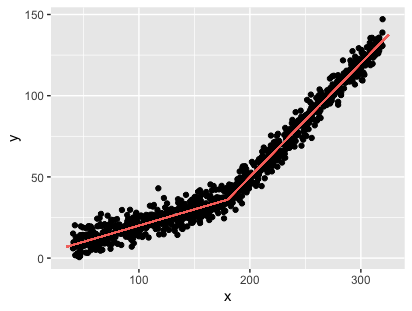
\includegraphics[width = 4 in]{Plot1_1.png}
    \caption{Data from a segmented regression model with 1 predictor and 1 breakpoint}
\end{figure}

Notice that we could easily extend such a model to multiple predictors ($X_1, X_2, \cdots$), each with more than one breakpoints ($\psi_{11}, \psi_{12}, \cdots$) and their respective slope changes ($\delta_{11}, \delta_{12}, \cdots$). Figure 1.2 illustrates a model with one predictor and three breakpoints.

\begin{figure}
    \centering
    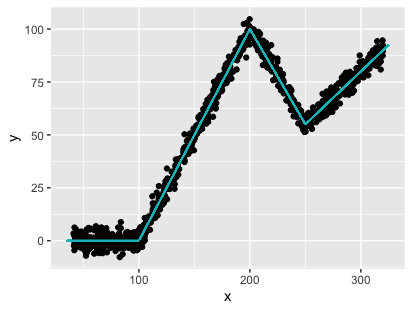
\includegraphics[width = 4 in]{Plot1_2.png}
    \caption{Data from a segmented regression model with 1 predictor and 3 breakpoints}
\end{figure}

With model (1.1), we assume that we know the location of the breakpoint $\psi$, and prespecify it before fitting the model. However, in real-world scenarios, the true locations of breakpoints are almost always unknown, which means we must estimate the breakpoints. We briefly discuss this in the section below.
 
\section{Estimating Breakpoints in Segmented Regression}

The theory of breakpoint estimation in segmented regression (also referred to as ``broken-stick regression'', ``multi-phase regression'', etc.) was first discussed in Hudson (1966) \cite{DH1966} and refined by Hinkley (1969) \cite{DH1969}, both of whom used likelihood theory to derive the asymptotic distribution of the estimate of location of the unknown breakpoint $\psi$ in Equation (1.1). 

However, because log-likelihood functions in segmented regression models are not continuously differentiable, the usual regularity conditions governing likelihood theory results are not met. This creates peculiarities and challenges in the estimation of $\psi$: for instance, when the actual relationship between the outcome and the predictor has fewer segments than postulated, not all slope estimates are asymptotically normal, nor is the likelihood ratio statistic distributed asymptotically $\chi^2$ \cite{PL1980}. Moreover, specialized techniques are required to estimate unknown breakpoints due to the non-linearity of the breakpoint term in Equation (1.1) \cite{PF1975a, PF1975b}.

In this thesis, we first discuss the method utilized by Muggeo (2003), which approximates the non-linear term in Equation (1.1) using a first-order Taylor expansion around some initial known value $\psi^{(0)}$, in lieu of directly attempting to maximize the log-likelihood function \cite{VM2003}. This method is conceptually straightforward and computationally simple, and, with minor changes, capable of modeling multiple breakpoints at once. Then we focus on modifications and expansions introduced in Muggeo \textit{et al.} (2014), which enable the estimation of covariate-specific breakpoints. We discuss this briefly below and in more detail in Chapter 3 \cite{VM2014}.
 
\section{Covariate-specific Breakpoints and Segmented Generalized Linear Regression: A Preview}
 
In Sections 1.1 and 1.2, we outlined a segmented regression framework with fixed breakpoints: that is, regardless of how many breakpoints exist in the model, the breakpoints are constants. However, for practical purposes, we may wish to include breakpoints that are functionally associated with some variable, which we express in a two-stage formulation as
\begin{align}
    y_i &= \beta_0 + \beta_1 x_i + \delta_1 (x_i - \psi_i)_+ + \epsilon_i \\
    \psi_i &= g(\bm{\kappa}; z_i),
\end{align}
where $Z = z_i$ is a variable that determines the location of the breakpoints $\psi_i$ through a potentially multidimensional paramter $\bm{\kappa}$, and $g(\cdot)$ is a function that maps the range of $Z = z_i$ to the range of $X = x_i$. It is worth pointing out that there is no restriction that $Z$ be a different variable than $X$; that is, a predictor of interest could also affect locations of breakpoints.

This additional layer of flexibility in the location of the breakpoint allows us to model segmented regression relationships with different breakpoints for subjects with different values of an additional covariate. Thus, the breakpoints estimated under this framework are referred to as ``covariate-specific breakpoints'' in this thesis. 

Furthermore, since the association between the outcome and the covariates in many scenarios need not be linear, it is also of interest to extend the estimation of covariate-specific breakpoints to generalized linear models:
\begin{align}
    h(\mathbb{E}[y_i]) &= \beta_0 + \beta_1 x_i + \delta_1 (x_i - \psi_i)_+ \\
    \psi_i &= g(\bm{\kappa}; z_i)
\end{align}

where $h(\cdot)$ is the link function in the segmented generalized linear model. We elaborate on both topics above in Section 3.2.

% ========== Chapter 2
 
\chapter{Cardiovascular Disease, The MESA Study, and Left Ventricular Hypertrophy (LVH): \\ A Scientific Introduction}

\section{Cardiovascular Disease and The MESA Study}
Cardiovascular disease (CVD), a family of diseases that affects the heart and the blood vessels, has been the leading cause of death in the United States since the 1960s \cite{JD2014}. It is also the leading cause of death worldwide, with a death toll of 17.9 million in 2016 \cite{WHO}. With such a tremendous impact on the physical wellbeing of humans around the world, CVD has been the focus of many large-scale clinical studies, including the Framingham Heart Study (FHS), the Cornell China Study, and the Multi-Ethnic Study of Atherosclerosis (MESA).

The Multi-Ethnic Study of Atherosclerosis (MESA) is a prospective cohort study initiated in July 2000 to study the epidemiology of subclinical CVD, with a study cohort of 6,814 subjects aged 45-84 years selected from six areas of the United States (Baltimore, Md.; Chicago, Ill.; Forsyth County, N.C.; Los Angeles County, Calif.; New York, N.Y.; and St. Paul, Minn.). The ethnic composition of the participants is 38\% White, 28\% African-American, 23\% Hispanic, and 11\% Asian, predominantly of Chinese descent. All subjects were free of clinically evident CVD at enrollment. The study's primary aims include determining risk factors associated with progression of CVD, both from no CVD to subclinical CVD and from subclinical CVD to clinical CVD. It also investigates ethnic, age, and sex differences in the prevalence, risk of progression, and rates of clinical CVD \cite{MESA}.

\section{Left Ventricular Hypertrophy and Its Clinical Quantification}

One of the most important factors that contribute to cardiovascular diseases in general is left ventricular hypertrophy (LVH), which is the enlargement and thickening of the walls of left ventricle, the main pumping chamber of the heart. LVH can develop in response to certain factors, such as hypertension or aortic stenosis. Those factors cause the workload of left ventricle to increase, which further thickens the muscles in the left ventricle wall. The size of the left ventricle may also increase. Consequently, the enlarged heart muscle may lose elasticity and eventually fail to pump with adequate force \cite{LVH}.

Many sequelae and complications associated with LVH are severe: stroke \cite{PV2006}, cardiac failure \cite{AG2006}, and dementia \cite{ARICNCS} are some examples. Therefore, accurately detecting the presence of LVH and quantifying its severity are of critical importance in cardiovascular research and clinical practice.

Currently, the most accurate way to measure left ventricular (LV) mass is cardiac magnetic resonance imaging (MRI), as opposed to earlier methods such as electrocardiography (ECG) and echocardiography (echo) \cite{CMRI}. The mass value obtained from the procedure is then used to determine whether a patient has LVH or not. However, heart mass and LV mass tend to be positively correlated with body mass and height, and there is ample evidence that males have higher LV masses compared to females, especially after puberty \cite{GdS1995}. Thus, adjusting for those factors is critical in ensuring that LVH is appropriately and accurately diagnosed.

A variety of clinical parameters have been developed to adjust for body size measures in the diagnosis of LVH. One is left ventricular mass divided by body surface area (LVM/BSA). However, it was found to underestimate the prevalence of LVH for obese patients. Furthermore, the most-commonly used formula used to calculate BSA (Dubois and Dubois regression) is based on only nine cadaveric patients reported more than 100 years ago, in 1916. Therefore, the validity and appropriateness of such an index are questionable \cite{AA2012}. There have also been proposals to index LVM by height (LVM/$h$). Subsequent observations on non-linearity of the association between body height and LVM inspired the development of allometric indices in the diagnosis of LVH, such as left ventricular mass indexed by height raised to the 2.7$^{th}$ power, LVM/$h^{2.7}$. Other researchers suggested exponents of 1.7, 2, and 2.13 to be used in the allometric indexing of left ventricular mass by height \cite{AA2012}.

However, the aforementioned allometric indices were developed based on echocardiography measurements and make geometric assumptions about the shape of the left ventricle. Such assumptions are somewhat crude approximations of left ventricular mass, due to the fact that the left ventricle is irregularly shaped. Lack of interpretability is another critical problem, especially when the body height is raised to a non-integer exponent in allometric indices. Furthermore, despite the clear physiological differences between males and females in heart growth and development, there is no straightforward way to provide sex-specific indices in the allometric indices above.

Brumback \textit{et al.} (2010) developed and described several newer allometric indices, including percent-predicted LV mass based on height and gender (ppLVmass$_H$) and percent-predicted LV mass based on height, weight, and gender (ppLVmass$_{HW}$), to adjust for both body size and sex in the diagnosis of LVH \cite{LB2010}. They used linear regression with log-transformed LV mass as the outcome and log-transformed height and/or log-transformed weight as predictors to derive those indices, while adjusting for gender. As a result, for example, a ppLVmass$_H$ of 1 corresponds to an LV mass equal to that predicted based on height and gender. They defined LVH as having a LV mass index that is greater than or equal to the empirical 95$^{th}$ percentile of a healthy sample based on prior research. These indices represent a marked improvement over past iterations of allometric indices because both gender and height have been modeled accurately, and the resulting ratio has a natural interpretation as a percentage of the predicted value. Nevertheless, the prevalence of LVH need not to be 5\% in a healthy population \cite{DM2019}.

In this thesis, we propose an alternative approach to defining left ventricular enlargement without imposing any restrictions on the prevalence in a healthy population, which is unknown. Given a set of baseline covariates such as gender and BMI, we instead estimate the point at which left ventricular mass begins to lead to increased risk of cardiovascular disease or death for that subjects with particular values of covariates. This is achieved by modeling our outcome as a segmented function of LV mass, and estimate covariate-specific breakpoints for all subjects using techniques introduced in Chapters 1.2 and 1.3.

% ========== Chapter 3
 
\chapter{Methods}

This chapter includes methods to estimate breakpoints in segmented linear regression and segmented generalized linear models. Chapter 3.1 introduces the estimation of one or more breakpoints that do not vary by participant level covariates (which we refer to as ``simple breakpoints'' for the rest of this thesis), whereas Chapter 3.2 outlines estimation of covariate-specific breakpoints. The methods illustrated here were originally developed by Muggeo \cite{VM2003, VM2014}, and the bootstrap restarting algorithm is explained in more detail in Wood (2001) \cite{SW2001}.
 
\section{Estimating One or More Simple Breakpoints}

\subsection{Estimating One Simple Breakpoint}

As introduced in Chapter 1.1, a segmented linear regression model with one simple breakpoint takes the following form:
\begin{align}
    y_i = \beta_0 + \beta_1 x_i + \delta_1 (x_i - \psi)_+ + \epsilon_i.
\end{align}
It is evident that the $\delta_1 (x_i - \psi)_+$ term, which corresponds to the slope change after the unknown simple breakpoint, is not linear due to the positive part function $(\cdot)_+$. Therefore, standard likelihood theory does not apply to this problem.

To overcome this issue, we perform a first-order Taylor series expansion of the $\delta_1 (x_i - \psi)_+$ term around some initial guess, $\psi^{(0)}$:
\begin{align}
    \delta_1 (x_i - \psi)_+ &\approx \delta_1 [(x_i - \psi^{(0)})_+ + (\psi - \psi^{(0)}) \dfrac{\partial}{\partial\psi} (x_i - \psi)_+ \Bigr|_{\psi = \psi^{(0)}}] \nonumber \\
    &= \delta_1 [(x_i - \psi^{(0)})_+ + (\psi - \psi^{(0)})(-1)I(x_i - \psi^{(0)})].
\end{align}

If we combine (3.1) and (3.2), we obtain
\begin{align}
    y_i &= \beta_0 + \beta_1 x_i + \delta_1 (x_i - \psi^{(0)})_+ + \delta_1 (\psi - \psi^{(0)})(-1)I(x_i - \psi^{(0)}) + \epsilon_i \nonumber \\
    &\equiv \beta_0 + \beta_1 x_i + \delta_1 (x_i - \psi^{(0)})_+ + \gamma_1(-I(x_i - \psi^{(0)})) + \epsilon_i,
\end{align}
while defining $\gamma_1 = \delta_1 (\psi - \psi^{(0)})$. 

We can obtain maximum likelihood estimates for each of the parameters in equation (3.3), including $\Hat{\delta_1}$ and $\Hat{\gamma_1}$. By the definition of $\gamma_1$, we can write
\begin{align}
    \Hat{\psi} = \dfrac{\Hat{\gamma_1}}{\Hat{\delta_1}} + \psi^{(0)}.
\end{align}

With equation (3.4), we can construct an algorithm that estimates all parameters in equation (3.3), as follows:

\begin{enumerate}
\begin{mybox}
    \item Fix $\psi^{(s)}$. Compute $U^{(s)} \equiv (x_i - \psi^{(s)})_+$ and $V^{(s)} \equiv -I(x_i > \psi^{(s)})$.
    \item Fit the model $y = \beta_0 + \beta_1 x_i + \delta_1 U^{(s)} + \gamma_1 V^{(s)} + \epsilon_i$. Obtain $\Hat{\beta_0}, \Hat{\beta_1}, \Hat{\delta_1}$, and $\Hat{\gamma_1}$.
    \item Obtain an updated estimate of $\psi$, $\psi^{(s+1)}$, by Equation (3.4).
\end{mybox}
    \captionof{enumcnt}{An iterative algorithm to estimate a single breakpoint in a segmented linear model}
\end{enumerate}

While this algorithm is not guaranteed to converge, it provides maximum likelihood estimates for all parameters in the model at convergence if it does converge \cite{BT1962}. Furthermore, the algorithm has been shown to be exact, and thus will always converge in a deterministic model, given that the breakpoint actually exists. In practice, an initial guess $\psi^{(0)}$ is usually obtained by visual inspection of a scatterplot of $Y$ versus $X$ \cite{VM2003}.

\subsection{Estimating Multiple Simple Breakpoints}

It is conceivable that more than one simple breakpoint may exist in the relationship between the outcome and the predictor. We could express a segmented regression model with one predictor and $k$ simple breakpoints as follows (see, for example, Figure 1.2 for three breakpoints in $X$):
\begin{align}
    y_i &= \beta_0 + \beta_1 x_i + \delta_1 (x_i - \psi_1)_+ + \delta_2 (x_i - \psi_2)_+ \cdots + \delta_k (x_i - \psi_k)_+ + \epsilon_i \nonumber \\
      &= \beta_0 + \beta_1 x_i + \sum_{j = 1}^k \delta_j (x_i - \psi_j)_+ + \epsilon_i,
\end{align}
where without loss of generality $\min_i x_i < \psi_1 < \psi_2 < \cdots < \psi_k < \max_i x_i$ denote $k$ breakpoints in the predictor $X$. It is worth noting that $\beta_1$ represents the ``first slope'' for $x_i < \psi_1$, and each of the $\delta_j$ represents the difference between slopes before and after breakpoint $\psi_j$. As a result, for $\psi_k < x_i < \psi_{k+1}$, the slope is $\beta_1 + \sum_{j=1}^k \delta_j$ for some $k \in \mathbb{N}^*$.

Similar first-order Taylor series expansions as Equation (3.2), with $\psi_1^{(0)}, \psi_2^{(0)}, \cdots, \psi_k^{(0)}$ as initial guesses for $\psi_1, \psi_2, \cdots, \psi_k$, yield
\begin{align}
    y_i &\approx \beta_0 + \beta_1 x_i + \delta_1 U_1^{(0)} + \gamma_1 V_1^{(0)} + \delta_2 U_2^{(0)} + \gamma_2 V_2^{(0)} + \cdots + \delta_k U_k^{(0)} + \gamma_k V_k^{(0)} + \epsilon_i \nonumber \\
    &= \beta_0 + \beta_1 x_i + \sum_{j=1}^k \delta_j U_j^{(0)} + \sum_{j=1}^k \gamma_j V_j^{(0)} + \epsilon_i,
\end{align}
where $U_j^{(0)} \equiv (x_i - \psi_j^{(0)})_+$ and $V_j^{(0)} \equiv -I(x_i - \psi_j^{(0)})$. Similar to (3.3), $\gamma_j = \delta_j (\psi_j - \psi_j^{(0)})$. Subsequently, we can write
\begin{align}
    \Hat{\psi_j} = \dfrac{\Hat{\gamma_j}}{\Hat{\delta_j}} + \psi_j^{(0)},
\end{align}

and construct an algorithm similar to Algorithm 3.1 to estimate all $k$ breakpoints in Equation (3.5).

While in theory it is possible to fit any number of breakpoints in a predictor, trying to fit too many breakpoints (typically more than 3 or 4) in a predictor often leads to overfitting. Other models, such as smoothing splines, should be considered instead to avoid overfitting of the data.
 
\section{Covariate-specific Breakpoints: Estimating Breakpoints Differing by Participant Level Covariates}

\subsection{Covariate-specific Breakpoint Model and Parameterization of the Breakpoint}
 
In Chapter 1.3, we provided a preview of covariate-specific breakpoints by defining a segmented regression model with the breakpoint parameter $\psi = \psi_i$ as a function of some variable $Z = z_i$. For illustration purposes, we express the simplest scenario, with one predictor of interest $X = x_i$, one breakpoint $\psi_i$, and a single variable $Z = z_i$ that determines the location of the breakpoint without influencing the outcome, in which case Equations (1.2) and (1.3) becomes
\begin{align}
    y_i &= \beta_0 + \beta_1 x_i + \delta_1 (x_i - \psi_i)_+ + \epsilon_i \\
    \psi_i &= g(\bm{\kappa}; z_i).
\end{align}

We note that variable $Z$ may or may not be identical to $X$, and the support of $Z$ could be either continuous or discrete. $\bm{\kappa} = (\kappa_0, \kappa_1, \cdots, \kappa_h)$ is an $(h+1)$-dimensional parameter through which the variable $Z$ affects the location of the breakpoint.

Alternatively, it is possible that in addition to $Z$ determining the location of the breakpoint, another variable $W = w_i$ determines the slope change after the breakpoint. For the sake of simplicity, we assume that $W$ appears as a linear parameter in the slope change. In this case, the model could be written as follows:
\begin{align}
    y_i &= \beta_0 + \beta_1 x_i + (\delta_{10} + \delta_{11} w_i) (x_i - \psi_i)_+ + \epsilon_i \\
    \psi_i &= g(\bm{\kappa}; z_i).
\end{align}

In either case, it is expected that function $g(\cdot)$ maps the support of $Z$ to the support of $X$. For now, we assume the observed support of $X$ to be $[a_1, a_2]$ and that $\bm{\kappa} = (\kappa_0, \kappa_1)$ is 2-dimensional (i.e. we only have one breakpoint-varying covariate). Then the following scaled and shifted logistic function always satisfies the above condition:
\begin{align}
    g(\bm{\kappa}; z_i) &= \dfrac{a_1 + a_2 e^{\kappa_0 + \kappa_1 z_i}}{1 + e^{\kappa_0 + \kappa_1 z_i}} \\
    &\equiv \dfrac{a_1 + a_2 e^{\eta_i}}{1 + e^{\eta_i}},
\end{align}
where $\eta_i \equiv \kappa_0 + \kappa_1 z_i$. Here, $\kappa_0$ could be interpreted as the location of the breakpoint, on the logit scale, when $z = 0$, whereas $\kappa_1$ is the slope on the logit scale that affects the location of the breakpoint. While other functions, such as a linear function $g(z_i) = k_0 + k_1 z_i$, could also be used for $g(\cdot)$, the estimated breakpoint locations may not always fall between minimum and maximum of observed values of $X$, and such results could be difficult to interpret.

We now illustrate methods to estimate the location of the breakpoint variable for both cases above.

\subsection{Covariate in Breakpoint Only}

We refer to the model defined in Equations (3.8) and (3.9) as ``covariate in breakpoint only'' model, because only $\psi_i$ is a function of covariate $Z = z_i$. The slope change after the breakpoint, $\delta_1$, is not a function of $Z$. We define $\eta_i = \kappa_0 + \kappa_1 z_i$ as before.

We first combine Equations (3.8) and (3.9): 
\begin{align}
    y_i &= \beta_0 + \beta_1 x_i + \delta_1 (x_i - g(\bm{\kappa}; z_i))_+ + \epsilon_i.
\end{align}

Similar to what we did in Chapter 3.1.1, we then perform a first-order Taylor series expansion of the $\delta_1 (x_i - \psi_i)_+ \equiv \delta_1 (x_i - g(\bm{\kappa}; z_i))_+$ term around some initial guess, $\bm{\kappa^{(0)}}$:
\begin{align}
    \delta_1 (x_i - g(\bm{\kappa}; z_i))_+ &\approx \delta_1 [(x_i - g(\bm{\kappa^{(0)}}; z_i))_+ + (\bm{\kappa} - \bm{\kappa^{(0)}})^T \dfrac{\partial}{\partial \bm{\kappa}} (x_i - g(\bm{\kappa^{(0)}}; z_i))_+ \Bigr|_{\bm{\kappa} = \bm{\kappa^{(0)}}}].
\end{align}

We evaluate the partial derivative of $f_i \equiv (x_i - g(\bm{\kappa^{(0)}}; z_i))_+$ on $\bm{\kappa}$:
\begin{align}
    \dfrac{\partial f_i}{\partial \bm{\kappa}} \Bigr|_{\bm{\kappa} = \bm{\kappa^{(0)}}} &= \dfrac{\partial f_i}{\partial g} \dfrac{\partial g}{\partial \eta_i} \dfrac{\partial \eta_i}{\partial \bm{\kappa}} \Bigr|_{\bm{\kappa} = \bm{\kappa^{(0)}}} \nonumber \\
    &= -I(x_i > \psi_i) \dfrac{e^{\eta_i} (a_2 - a_1)}{(1+e^{\eta_i})^2} \dfrac{\partial \eta_i}{\partial \bm{\kappa}} \Bigr|_{\bm{\kappa} = \bm{\kappa^{(0)}}}. \nonumber
\end{align}

We define $V_i \equiv -I(x_i > \psi_i)$ and $D_i \equiv \dfrac{e^{\eta_i} (a_2 - a_1)}{(1+e^{\eta_i})^2}$ and evaluate component-wise,
\begin{align}
    \dfrac{\partial f_i}{\partial \kappa_0} &= V_i D_i \\
    \dfrac{\partial f_i}{\partial \kappa_1} &= V_i D_i z_1.
\end{align}

Defining $U_i \equiv (x_i - g(\bm{\kappa}; z_i))_+ = (x_i - \psi_i)_+$ and $z_0 \equiv 1$, using tilde to denote approximate values, and combining Equations (3.15), (3.16), and (3.17) yields
\begin{align}
    \delta_1 (x_i - \psi_i)_+ &\approx \delta_1 \Tilde{U}_i + \delta_1 (\kappa_0 - \Tilde{\kappa}_0) \Tilde{V}_i \Tilde{D}_i + \delta_1 (\kappa_1 - \Tilde{\kappa}_1) \Tilde{V}_i \Tilde{D}_i z_i.
\end{align}

Suppose we could obtain an approximate value of $\delta_1, \Tilde{\delta}_1$, then we could rewrite Equation (3.18) as:
\begin{align}
    \delta_1 (x_i - \psi_i)_+ &\approx \delta_1 \Tilde{U}_i + (\kappa_0 - \Tilde{\kappa}_0) \Tilde{\delta}_1 \Tilde{V}_i \Tilde{D}_i + (\kappa_1 - \Tilde{\kappa}_1) \Tilde{\delta}_1 \Tilde{V}_i \Tilde{D}_i z_i \nonumber \\
    &\equiv \delta_1 \Tilde{U}_i + \kappa_0 \Tilde{G}_{0i} + \kappa_1 \Tilde{G}_{1i} + \{ -\Tilde{\kappa}_0 \Tilde{G}_{0i} -\Tilde{\kappa}_1 \Tilde{G}_{1i}\}.
\end{align}

We observe that in Equation (3.19), the terms in the curly bracket are known terms, which we could treat as an offset. With this equation, we have completed a first-order Taylor series expansion. We introduce the algorithm used to fit this model iteratively in Section 3.2.4.

\subsection{Covariates in Breakpoint and Slope}
We refer to the model defined in Equations (3.10) and (3.11) as ``covariates in breakpoint and slope'' model, because both $\psi_i$ and $\delta_{1i} \equiv \delta_{10} + \delta_{11} w_i$ are functions of breakpoint-varying covariates $Z = z_i$ and $W = w_i$. Again, we define $\eta_i = \kappa_0 + \kappa_1 z_i$ as before.

Likewise we first combine Equations (3.10) and (3.11):
\begin{align}
    y_i &= \beta_0 + \beta_1 x_i + (\delta_{10} + \delta_{11} w_i) (x_i - g(\bm{\kappa}; z_i))_+ + \epsilon_i.
\end{align}

Using identical arguments and variable definitions as we did in Section 3.2.2, we perform a first-order Taylor series expansion on the term $(\delta_{10} + \delta_{11} z_i) (x_i - g(\bm{\kappa}; z_i))_+$ and write:
\begin{align}
    \delta_{10} (x_i - \psi_i)_+ + \delta_{11} (x_i - \psi_i)_+ w_i &\approx \delta_{10} \Tilde{U}_i + \delta_{11} \Tilde{U}_i w_i + (\kappa_0 - \Tilde{\kappa}_0) \delta_{10} \Tilde{V}_i \Tilde{D}_i + \nonumber \\
    & \hspace{0.22in} (\kappa_0 - \Tilde{\kappa}_0) \delta_{11} \Tilde{V}_i \Tilde{D}_i w_i + (\kappa_1 - \Tilde{\kappa}_1) \delta_{10} \Tilde{V}_i \Tilde{D}_i z_i + \nonumber \\
    & \hspace{0.22in} (\kappa_1 - \Tilde{\kappa}_1) \delta_{11} \Tilde{V}_i \Tilde{D}_i z_i w_i. \nonumber
\end{align}

Again, assuming that we could obtain approximate values for $\delta_{10}$ and $\delta_{11}$, then the previous equation evaluates to:
\begin{align}
    \delta_{10} (x_i - \psi_i)_+ + \delta_{11} (x_i - \psi_i)_+ w_i &\approx \delta_{10} \Tilde{U}_i + \delta_{11} \Tilde{U}_i w_i + (\kappa_0 - \Tilde{\kappa}_0) \{\Tilde{\delta}_{10} \Tilde{V}_i \Tilde{D}_i + \Tilde{\delta}_{11} \Tilde{V}_i \Tilde{D}_i w_i \} + \nonumber \\
    & \hspace{0.22in} (\kappa_1 - \Tilde{\kappa}_1) \{\Tilde{\delta}_{10} \Tilde{V}_i \Tilde{D}_i z_i + \Tilde{\delta}_{11} \Tilde{V}_i \Tilde{D}_i z_i w_i \} \nonumber \\
    &\equiv \delta_{10} \Tilde{U}_i + \delta_{11} \Tilde{U}_i w_i + \kappa_0 \Tilde{G}_{0i} + \kappa_1 \Tilde{G}_{1i} + \{ -\Tilde{\kappa}_0 \Tilde{G}_{0i} -\Tilde{\kappa}_1 \Tilde{G}_{1i}\}.
\end{align}

Similar to Equation (3.19), this equation also has an offset term that is known. We detail how to fit both models in Section 3.2.4 below.

\subsection{Model Estimation and Algorithm}
We first observe that Equation (3.19) is a special case of Equation (3.21) by setting $w_i = 0$ for all $i$. Thus, we focus our discussion on an algorithm that fits the ``covariates in breakpoint and slope'' model, which will also pertain to the ``covariates in breakpoint only'' model.

With Equations (3.19) and (3.21) containing only linear predictors, estimation of the two models introduced in the beginning of Chapter 3 is now feasible. Similar to what we described in Chapter 3.1.1, we assume that we could obtain an approximation of breakpoint for each subject $i = 1, 2, \cdots, n$. For instance, we could set $\Tilde{\psi}_i = \Tilde{\psi}^{(0)}$ for all subjects initially. An example of a more sophisticated guess is setting different $\Tilde{\psi}$'s for subjects with breakpoint-varying covariate $z_i$ in different quartiles, which we will briefly discuss in Chapter 6.

It is worth mentioning that we have also assumed that we could obtain initial approximations for $\kappa_0, \kappa_1, \delta_{10}$, and $\delta_{11}$. We first address those assumptions in the setting that the initial approximation of breakpoints is identical for all subjects (i.e. $\Tilde{\psi}_i = \Tilde{\psi}^{(0)}$ for all $i$) via a visual inspection of the scatterplot of $Y$ versus $X$. Under that assumption, $\Tilde{\kappa}_0 = \log \left(\dfrac{\Tilde{\psi}^{(0)} - a_1}{a_2 - \Tilde{\psi}^{(0)}}\right)$, and $\Tilde{\kappa}_1 = 0$ because all subjects have the same initial approximated breakpoint. To obtain initial estimates for $\delta_{10}$ and $\delta_{11}$, we fit the following linear model:
\begin{align}
    y_i &= \beta_0 + \beta_1 x_i + \delta_{10} U_i + \delta_{11} U_i w_i,
\end{align}
by using $\Tilde{U}_i = (x_i - \Tilde{\psi}_i)_+$ to approximate $U_i$. Thus we could obtain $\Tilde{\delta}_{10}$ and $\Tilde{\delta}_{11}$. Combining Equations (3.20) and (3.21) yields:
\begin{align}
    y_i = \beta_0 + \beta_1 x_i + \delta_{10} \Tilde{U}_i + \delta_{11} \Tilde{U}_i w_i + \kappa_0 \Tilde{G}_{0i} + \kappa_1 \Tilde{G}_{1i} + \Tilde{O}_i,
\end{align}
where $\Tilde{O}_i = -\Tilde{\kappa}_0 \Tilde{G}_{0i} -\Tilde{\kappa}_1 \Tilde{G}_{1i}$ represents a known offset term as discussed above. We now use the following algorithm:
\begin{enumerate}
\begin{mybox}
    \item With approximate values $\Tilde{\kappa}_0, \Tilde{\kappa}_1, \Tilde{\psi}_i, \Tilde{\delta}_{10}, \Tilde{\delta}_{11}$, compute $\Tilde{U}, \Tilde{U}w, \Tilde{G}_0, \Tilde{G}_1, \Tilde{O}$ by their definitions.
    \item Fit the model in Equation (3.23).
    \item From the fitted model, obtain $\Hat{\kappa}_0$ and $\Hat{\kappa}_1$, and thus $\Hat{\eta_i} = \Hat{\kappa}_0 + \Hat{\kappa}_1 z_i$ and subsequently $\Hat{\psi}_i = \dfrac{a_1 + a_2 e^{\Hat{\eta_i}}}{1 + e^{\Hat{\eta_i}}}$. Also, obtain $\Hat{\delta}_{10}$ and $\Hat{\delta}_{11}$. \item Replace guesses for $\Tilde{\kappa}_0, \Tilde{\kappa}_1, \Tilde{\psi}_i, \Tilde{\delta}_{10}, \Tilde{\delta}_{11}$ with their estimates obtained in the previous step.
\end{mybox}
    \captionof{enumcnt}{An iterative algorithm to estimate covariate-specific breakpoints in a segmented linear model}
\end{enumerate}

We repeat steps 1-4 until the difference in log-likelihoods between two steps is smaller than some preset threshold. As with Algorithm 3.1, this algorithm is not guaranteed to converge, but will yield maximum likelihood estimates if it does converge \cite{VM2014}. We next discuss several possible extensions to the estimation procedure and this algorithm, as well as a solution to avoid reaching local maxima of the log-likelihood function, in the section below.

\subsection{The Bootstrap Restarting Algorithm}

As with other statistical methods that optimize an objective function, our method may have difficulty reaching the global maximum of a non-convex and multimodal log-likelihood. This difficulty could be caused by a variety of factors, including noisiness of the data and relatively small slope change after a breakpoint. In such cases, different initial values $\Tilde{\psi}^{(0)}$ will likely lead to different final results, which subsequently could result in non-convergence. 

The bootstrap restarting algorithm was found to be an effective approach to ``escape'' local maxima of the log-likelihood function in this estimation problem \cite{VM2003, SW2001}. We specify its steps as follows:
\begin{enumerate}
\begin{mybox}
    \item Use initial value $\Tilde{\bm{\kappa}}$ to fit the model in Equation (3.23). Denote the fitted breakpoint parameters as $\Hat{\bm{\kappa}}$. Record the value of log-likelihood function.
    \item Create $n$ nonparametric bootstrap samples of the original sample. Use $\Hat{\bm{\kappa}}$, the fitted breakpoint from the original sample, as the initial value for bootstrap samples. Denote the fitted breakpoint parameters from this step as $\Hat{\bm{\kappa}}^*_{(1)}, \Hat{\bm{\kappa}}^*_{(2)}, \cdots, \Hat{\bm{\kappa}}^*_{(n)}$.
    \item Refit the original sample with initial values $\Hat{\bm{\kappa}}^*_{(1)}, \Hat{\bm{\kappa}}^*_{(2)}, \cdots, \Hat{\bm{\kappa}}^*_{(n)}$ and obtain new fitted breakpoint parameters $\Hat{\bm{\kappa}}^{BR}_{(1)}, \Hat{\bm{\kappa}}^{BR}_{(2)}, \cdots, \Hat{\bm{\kappa}}^{BR}_{(n)}$. Record the values of log-likelihood function corresponding to all $n$ initial values.
    \item Find the maximum of $(n+1)$ values of log-likelihood function (1 value from Step 1 and $n$ values from Step 3) and use its corresponding fitted breakpoint parameters.
\end{mybox}
    \captionof{enumcnt}{Algorithm 3.2 with a bootstrap restarting approach to avoid local maxima of log-likelihood function}
\end{enumerate}

Similar to what we did in the previous section, we repeat steps 1-4 until the difference in log-likelihoods between two steps is smaller than some preset threshold. Muggeo suggested that it is sufficient to use $n = 10$ nonparametric bootstrap samples for each iteration. Since the bootstrap restarting algorithm cannot produce a worse fit than the original algorithm, we elect to use Algorithm 3.3 in lieu of Algorithm 3.2 in this thesis \cite{SW2001}. We find that the bootstrap restarting algorithm routinely produces errors in breakpoint estimates that are lower by roughly an order of magnitude when the data is noisy, when the slope change is small, or when the initial guesses for the breakpoints are severely misspecified.

\subsection{Additional Remarks}
So far we have only discussed models where the relationship between the outcome and the primary predictor of interest is (segmented) linear. Those models under most circumstances assume that the mean of the outcome variable is linear with normally distributed errors. However, in many practical applications, the outcome variable could take on other forms: binary outcome, count data, and observed survival time are some of the examples where generalized linear models are appropriate. We contend that we could apply Algorithm 3.1 to 3.3 with minimal modifications for generalized linear models, because the overall approach of the algorithms is to approximate a non-linear breakpoint term with Taylor series expansion, which does not concern the link function $h(\cdot)$.

The model and the algorithms could also easily accommodate more than one variable that affect the location of the breakpoint, as well as more than one variable that affect the slope change after the breakpoint. With $p$ variables $z_1, z_2, \cdots, z_p$ that affect the location of the breakpoint and $q$ variables $w_1, w_2, \cdots, w_q$, we could simply construct new variables that are similar to $\Tilde{G}_0$ and $\Tilde{G}_1$ in structure. The $p^{th}$ ``$G$-type''variable would be:
\begin{align}
    \Tilde{G}_p = \Tilde{\delta}_{p0} VDz_p + \Tilde{\delta}_{p1} VD z_p x_1 + \cdots + \Tilde{\delta}_{pq} VD z_p x_q
\end{align}

where $z_0 \equiv 1$ and $\Tilde{\delta}_{p0}, \Tilde{\delta}_{p1}, \cdots, \Tilde{\delta}_{pq}$ are coefficients of variables $\Tilde{U}, \Tilde{U}w_1, \cdots, \Tilde{U}w_q$. We could then obtain initial estimates of coefficients of ``$G$-type'' variables with an approach similar to what we described in Equation (3.22), and proceed with an appropriate algorithm introduced in Chapter 3.

% ========== Chapter 4
 
\chapter{Simulation Studies}

In this chapter, we present several simulation studies designed to evaluate the performance of algorithms outlined in Chapter 3 under various settings. In earlier chapters, we have stated that our primary statistical and scientific interest is estimating locations of covariate-specific breakpoints $\psi_i$, given an outcome variable $Y$, a primary predictor of interest $X$, a set of $p$ breakpoint-varying covariates $Z_1, Z_2, \cdots, Z_p$ (which we will refer to as ``\emph{$Z$-covariates}") and a set of $q$ covariates that impacts the slope change $W_1, W_2, \cdots, W_q$ (which we will refer to as ``\emph{$W$-covariates}"). We specify the model as follows:
\begin{align}
   y_i &= \beta_0 + \beta_1 x_i + (\delta_{10} + \delta_{11} w_{1i} + \cdots + \delta_{1q} w_{qi}) (x_i - \psi_i)_+ + \epsilon_i \\
    \psi_i &= \dfrac{a_1 + a_2 e^{\eta_i}}{1 + e^{\eta_i}} \\
    \eta_i &= \kappa_0 + \kappa_1 z_{1i} + \cdots + \kappa_p z_{pi},
\end{align}
where $a_1 = \min_i x_i$, $a_2 = \max_i x_i$, and $\epsilon_i \sim \mathcal{N}(0, \sigma^2)$.

We focus mainly on the performance of the estimated breakpoint $\Hat{\psi_i}$ under the following settings:
\begin{enumerate}
    \item No $Z$- or $W$-covariates. This translates to one simple breakpoint $\psi_i = \psi$ for all subjects and same slope change at breakpoint for all observations.
    \item One binary $Z$-covariate $Z = z_i \in \{0, 1\}$ and no $W$-covariates. This translates to two distinct groups in the sample, each with a unique breakpoint that all members in the group share; slope change remains the same for all observations.
    \item One continuous $Z$-covariate $Z = z_i \in \mathbb{R}$ and no $W$-covariates. This translates to observations with different $z_i$ values having different breakpoints; slope change remains the same for all observations.
    \item One continuous $Z$-covariate $Z = z_i \in \mathbb{R}$ and one distinct continuous $W$-covariate $W = w_i \in \mathbb{R}$. This translates to observations with different combinations of $(z_i, w_i)$ values having different breakpoints and slope change.
\end{enumerate}

We present numerical summaries of empirical distributions of both root mean squared error (RMSE $=\sqrt{\mathbb{E}[(\Hat{\psi_i} - \psi_i)^2]}$) and mean absolute error (MAE $=\mathbb{E}[\lvert \Hat{\psi_i} - \psi_i \rvert]$) to quantify method accuracy in each of the settings (except for Setting 1, where those two values are identical by definition). 

\section{Setting 1: One Simple Breakpoint, Constant Slope Change}
 We generate data from the following model (see Figure A.1, Appendix A for an example):
\begin{align*}
    y_i &= 0.2 x_i + \delta_1 (x_i - \psi_i)_+ + \epsilon_i \\
    \psi_i &= \psi
\end{align*}

where $x_i \sim U(40, 320), \epsilon_i \sim \mathcal{N}(0, \sigma^2)$ and $i = 1, 2, \cdots, N$. We set $N \in \{500, 2000\}, \psi \in \{180, 280\}, \delta_1 \in \{0.2, 0.5\}$, and $\sigma \in \{2, 10\}$. Furthermore, we set $\psi^{(0)} = \psi - 10$ as initial guesses; that is, $\psi^{(0)} = 170$ when $\psi = 180$, and $\psi^{(0)} = 270$ when $\psi = 280$ respectively. Those initial values mimic reasonable, but imperfect, guesses of the true breakpoint values, because it is feasible in practical applications to obtain initial guesses that are not too far from the ``truth'' via inspection of a scatterplot (or LOESS smoother curves of a scatterplot) of $Y$ versus $X$ \cite{VM2003, VM2014}. In Table 4.1 and Figure 4.1, we present distributions of the mean absolute error based on 1,000 replications of each possible combination of parameters noted above.

\begin{table}
\centering
\renewcommand\arraystretch{0.75}
\begin{tabular}{@{} lccccccc @{}} 
\toprule
    {Slope Change} & {$\psi$} & $\sigma$ & $N$ & \multicolumn{4}{c}{Sampling Distribution of} \\
    & & & & \multicolumn{4}{c}{MAE, $\mathbb{E}[\lvert \Hat{\psi_i} - \psi_i \rvert]$} \\
    \cmidrule(lr){5-8}
     & & & & Mean & Median & Q1 & Q3 \\
\midrule
    $\delta_1 = 0.2$ & 180 & 2 & 500 & 1.47 & 1.19 & 0.58 & 2.17 \\
                     &     &   & 2000 & 0.71 & 0.57 & 0.26 & 1.02  \\
                     &     & 10 & 500 & 8.44 & 7.22 & 3.40 & 11.56 \\
                     &     &    & 2000 & 3.91 & 3.12 & 1.36 & 5.63 \\
                     & 280 & 2 & 500 & 2.26 & 1.74 & 0.84 & 3.19 \\
                     &     &   & 2000 & 1.11 & 0.93 & 0.44 & 1.60 \\
                     &     & 10 & 500 & 15.34 & 10.04 & 4.97 & 16.80 \\
                     &     &    & 2000 & 6.42 & 5.01 & 2.40 & 8.52 \\
\midrule
    $\delta_1 = 0.5$ & 180 & 2 & 500 & 0.57 & 0.46 & 0.22 & 0.81  \\
                     &     &   & 2000 & 0.29 & 0.26 & 0.12 & 0.42 \\
                     &     & 10 & 500 & 3.12 & 2.66 & 1.29 & 4.32 \\
                     &     &     & 2000 & 1.41 & 1.16 & 0.54 & 2.05 \\
                     & 280 & 2 & 500 & 0.88 & 0.72 & 0.36 & 1.29 \\
                     &     &     & 2000 & 0.41 & 0.34 & 0.15 & 0.58 \\
                     &     & 10 & 500 & 5.33 & 4.56 & 2.08 & 7.68 \\
                     &     &     & 2000 & 2.35 & 1.97 & 0.86 & 3.35 \\    
\bottomrule
\end{tabular}
\caption{Distribution of Mean Absolute Error Based on 1,000 Replicates under Setting 1}
\end{table}

\begin{figure}
    \centering
    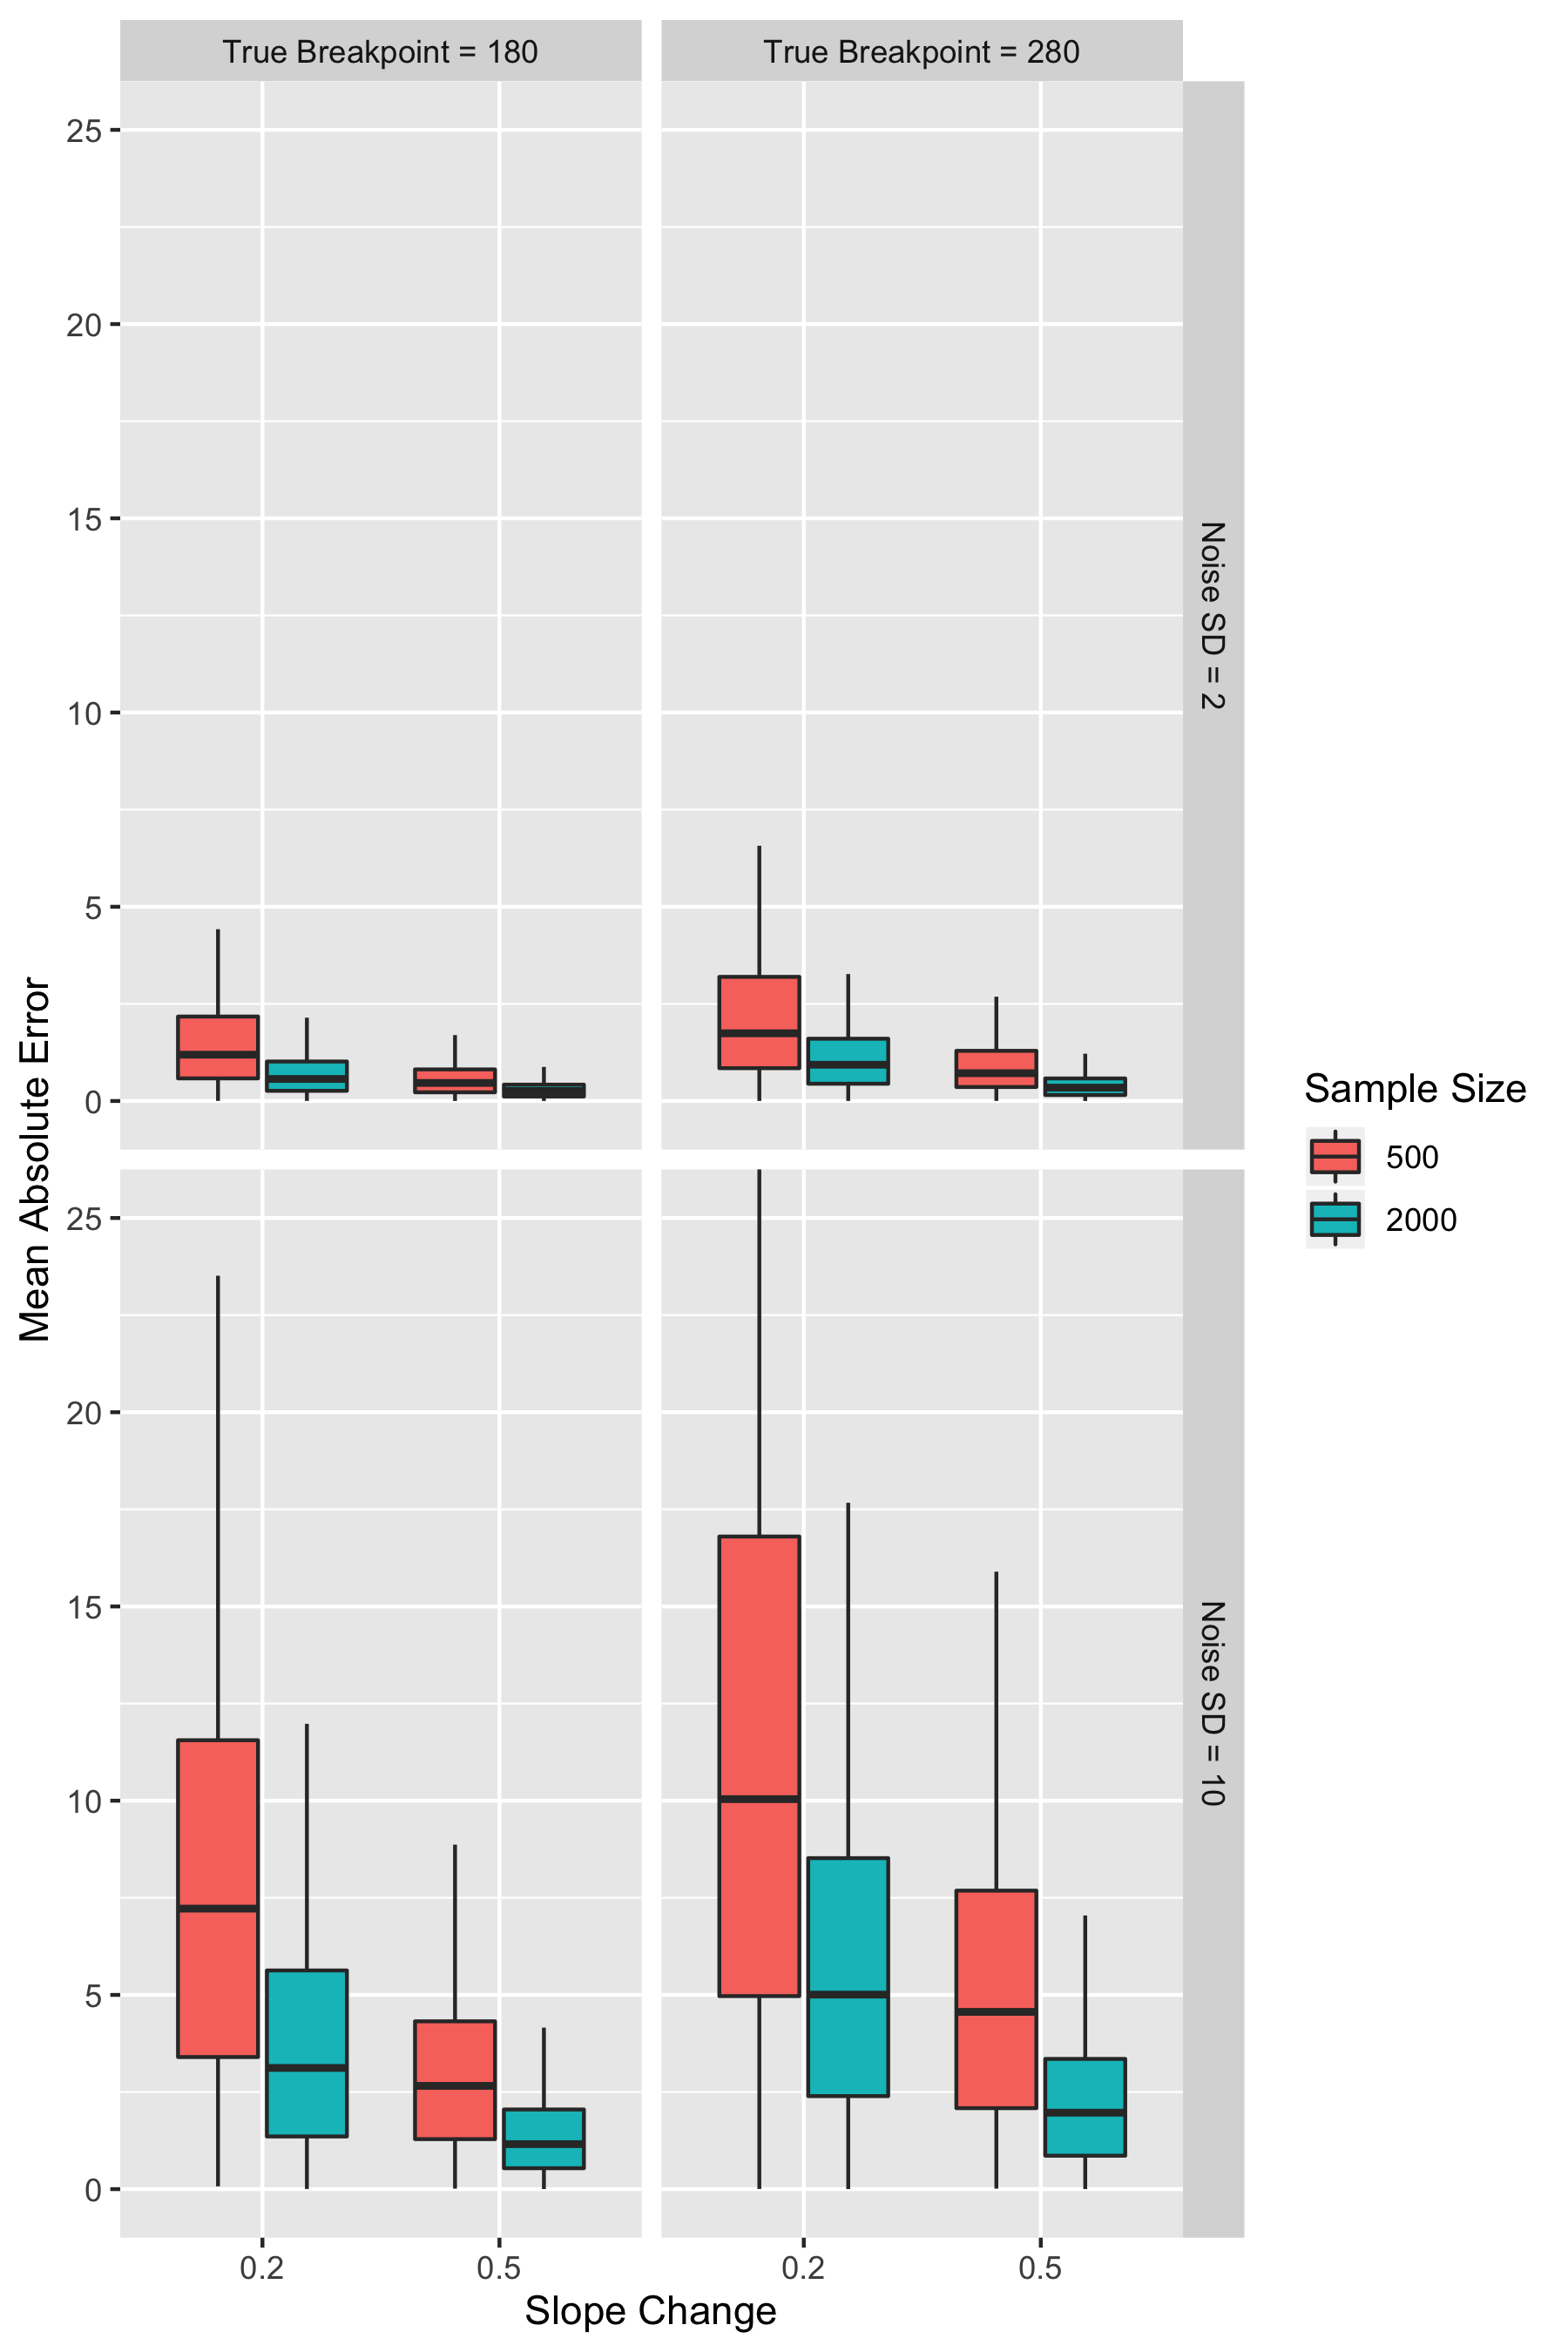
\includegraphics[width = 5.5 in]{Plot4_1.png}
    \caption{Boxplots of Distribution of Mean Absolute Error Based on 1,000 Replicates under Setting 1}
\end{figure}

We observe that given the same $\delta_1, \psi$, and $\sigma$, quadrupling the sample size (500 vs. 2000) results in about halving of the mean of MAE. It is also unsurprising to see that higher levels of noise in the outcome variable is related to larger MAEs. Moreover, it is more difficult to obtain accurate estimates when the true breakpoint location is closer to the upper (or lower) bounds of the range of $X$.

\section{Setting 2: Covariate-specific Breakpoint with Binary Covariate, Constant Slope Change}
We generate data from the following model (see Figure A.2, Appendix A for an example):
\begin{align*}
    y_i &= 0.2 x_i + \delta_1 (x_i - \psi_i)_+ + \epsilon_i \\
    \psi_i &= \dfrac{40 + 320 e^{\eta_i}}{1 + e^{\eta_i}} \\
    \eta_i &= z_{1i}
\end{align*}

where $x_i \sim U(40, 320), \epsilon_i \sim \mathcal{N}(0, \sigma^2)$ and $i = 1, 2, \cdots, N$. We set $N \in \{500, 2000\}, \delta_1 \in \{0.2, 0.5\}$, and $\sigma \in \{2, 10\}$ as before. We set $z_{1i} \sim k \cdot \text{Binomial}(n = N, p = 0.5)$, and let $k \in \{0.5, 1.5\}$; that is, a larger $k$ value corresponds to a larger distance between two breakpoints. Similar to what we did in Chapter 4.1, We set $\psi^{(0)} = \psi - 10$ as initial guesses for all observations. We contend that this is realistic in practice because we only have two different breakpoint values, whose values could be well-approximated by an inspection of a scatterplot (or LOESS smoother curves of a scatterplot) of $Y$ versus $X$. In Table 4.2 and Figure 4.2, we present distributions of mean absolute error based on 1,000 replications of each possible combination of parameters noted above.

\begin{table}
\centering
\renewcommand\arraystretch{0.75}
\begin{tabular}{@{} lccccccccccc @{}} 
\toprule
    {Slope Change} & {$k$} & $\sigma$ & $N$ & \multicolumn{4}{c}{Sampling Distribution of} & \multicolumn{4}{c}{Sampling Distribution of} \\
    & & & & \multicolumn{4}{c}{MAE, $\mathbb{E}[\lvert \Hat{\psi_i} - \psi_i \rvert]$} & \multicolumn{4}{c}{RMSE, $\sqrt{\mathbb{E}[(\Hat{\psi_i} - \psi_i)^2]}$}\\
    \cmidrule(lr){5-8} \cmidrule(lr){9-12}
     & & & & Mean & Median & Q1 & Q3 & Mean & Median & Q1 & Q3 \\
\midrule
    $\delta_1 = 0.2$ & 0.5 & 2 & 500 & 2.00 & 1.66 & 0.98 & 2.70 & 2.11 & 1.78 & 1.11 & 2.86 \\
                     &     &   & 2000 & 0.96 & 0.80 & 0.47 & 1.31 & 1.01 & 0.89 & 0.55 & 1.37  \\
                     &     & 10 & 500 & 9.61 & 7.89 & 4.45 & 13.02 & 10.25 & 8.56 & 4.90 & 13.86 \\
                     &     &    & 2000 & 4.87 & 4.08 & 2.29 & 6.62 & 5.15 & 4.38 & 2.53 & 6.96 \\
                     & 1.5 & 2 & 500 & 1.92 & 1.68 & 1.07 & 2.46 & 2.10 & 1.86 & 1.19 & 2.73 \\
                     &     &   & 2000 & 0.92 & 0.83 & 0.52 & 1.21 & 1.01 & 0.91 & 0.59 & 1.34 \\
                     &     & 10 & 500 & 9.73 & 8.38 & 5.36 & 12.47 & 10.63 & 9.45 & 5.81 & 13.82\\
                     &     &    & 2000 & 4.90 & 4.49 & 2.78 & 6.43 & 5.36 & 4.96 & 3.09 & 7.01 \\
\midrule
    $\delta_1 = 0.5$ & 0.5 & 2 & 500 & 0.79 & 0.65 & 0.38 & 1.09 & 0.83 & 0.72 & 0.41 & 1.14  \\
                     &     &   & 2000 & 0.39 & 0.33 & 0.20 & 0.54 & 0.42 & 0.36 & 0.22 & 0.56 \\
                     &     & 10 & 500 & 4.00 & 3.20 & 1.92 & 5.46 & 4.23 & 3.55 & 2.14 & 5.64 \\
                     &     &     & 2000 & 1.93 & 1.55 & 0.95 & 2.58 & 2.04 & 1.72 & 1.07 & 2.70 \\
                     & 1.5 & 2 & 500 & 0.78 & 0.69 & 0.44 & 1.03 & 0.85 & 0.76 & 0.48 & 1.13 \\
                     &     &     & 2000 & 0.38 & 0.33 & 0.21 & 0.52 & 0.42 & 0.36 & 0.24 & 0.57 \\
                     &     & 10 & 500 & 3.78 & 3.39 & 2.13 & 4.88 & 4.13 & 3.72 & 2.40 & 5.38 \\
                     &     &     & 2000 & 1.89 & 1.66 & 1.04 & 2.50 & 2.06 & 1.90 & 1.16 & 2.74 \\    
\bottomrule
\end{tabular}
\caption{Distribution of Mean Absolute Error and Root Mean Squared Error Based on 1,000 Replicates under Setting 2}
\end{table}

\begin{figure}
    \centering
    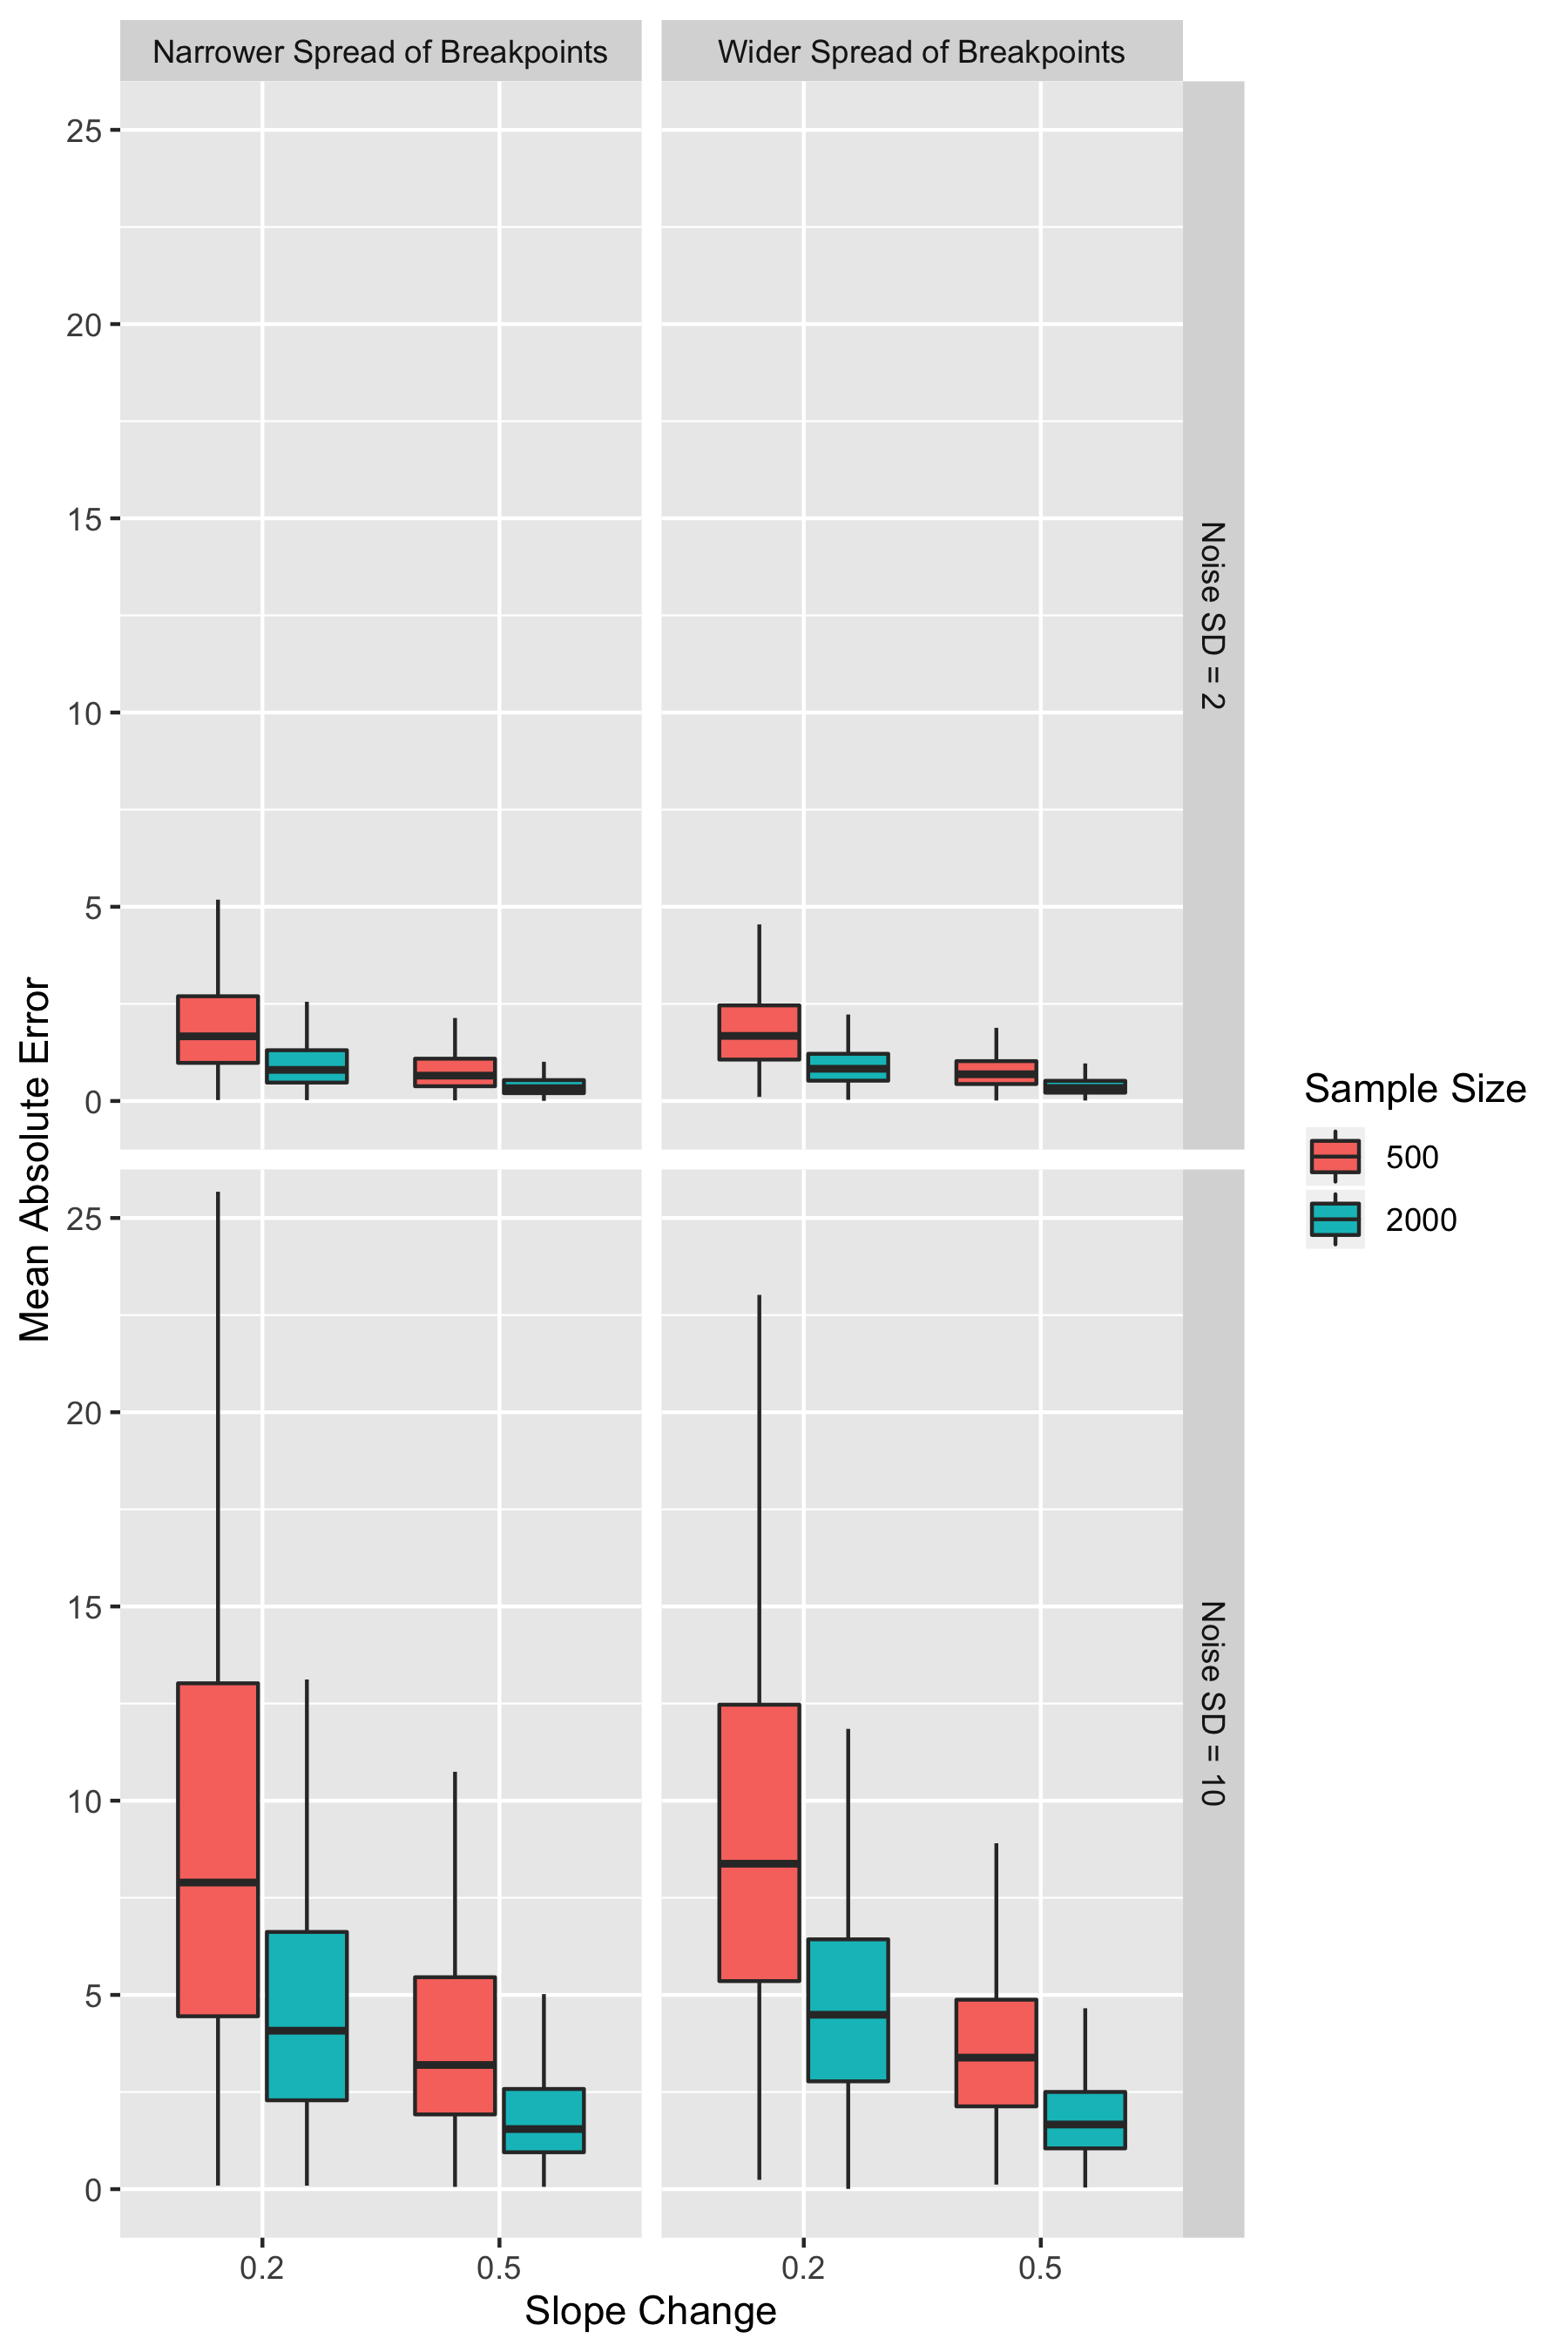
\includegraphics[width = 5.5 in]{Plot4_2.png}
    \caption{Boxplots of Distribution of Mean Absolute Error Based on 1,000 Replicates under Setting 2}
\end{figure}

The behavior of the (empirical) distributions of both MAE and RMSE is largely the same as that of Setting 1, with MAE being strictly less than RMSE (by Jensen's inequality). However, we observe that Setting 2 has higher MAEs in general compared to Setting 1. This is anticipated due to the inclusion of a binary $Z$-covariate.

\section{Setting 3: Covariate-specific Breakpoint with Continuous Covariate, Constant Slope Change}
We generate data from the following model (see Figure A.3, Appendix A for an example):
\begin{align*}
    y_i &= 0.2 x_i + \delta_1 (x_i - \psi_i)_+ + \epsilon_i \\
    \psi_i &= \dfrac{40 + 320 e^{\eta_i}}{1 + e^{\eta_i}} \\
    \eta_i &= z_{1i}
\end{align*}

where $x_i \sim U(40, 320), \epsilon_i \sim \mathcal{N}(0, \sigma^2)$ and $i = 1, 2, \cdots, N$. We set $N \in \{500, 2000\}, \delta_1 \in \{0.2, 0.5\}$, and $\sigma \in \{2, 10\}$ as before. We set $z_{1i} \sim \mathcal{N}(0, k^2)$, and let $k \in \{0.5, 1.5\}$; that is, a larger $k$ value corresponds to a larger spread of breakpoint locations. Because $z_1$ is drawn from a continuous distribution in this setting, each observation will have its unique breakpoint unless two observations have identical $z_1$ values. Thus, to avoid imposing extra assumptions about the relationship between $x_i$'s and $\psi_i$'s, we use $\psi_i = \text{median}(x) - 10 = 170$ for all observations as an initial guess. In Table 4.3 and Figure 4.3, we present distributions of mean absolute error based on 1,000 replications of each possible combination of parameters noted above.

\begin{table}
\centering
\renewcommand\arraystretch{0.75}
\begin{tabular}{@{} lccccccccccc @{}} 
\toprule
    {Slope Change} & {$k$} & $\sigma$ & $N$ & \multicolumn{4}{c}{Sampling Distribution of} & \multicolumn{4}{c}{Sampling Distribution of} \\
    & & & & \multicolumn{4}{c}{MAE, $\mathbb{E}[\lvert \Hat{\psi_i} - \psi_i \rvert]$} & \multicolumn{4}{c}{RMSE, $\sqrt{\mathbb{E}[(\Hat{\psi_i} - \psi_i)^2]}$}\\
    \cmidrule(lr){5-8} \cmidrule(lr){9-12}
     & & & & Mean & Median & Q1 & Q3 & Mean & Median & Q1 & Q3 \\
\midrule
    $\delta_1 = 0.2$ & 0.5 & 2 & 500 & 3.10 & 2.59 & 1.44 & 4.20 & 3.28 & 2.76 & 1.64 & 4.47 \\
                     &     &   & 2000 & 1.48 & 1.23 & 0.72 & 2.04 & 1.57 & 1.31 & 0.80 & 2.15  \\
                     &     & 10 & 500 & 15.14 & 11.96 & 6.86 & 20.10 & 16.17 & 13.17 & 7.79 & 21.28 \\
                     &     &    & 2000 & 7.71 & 6.08 & 3.41 & 10.65 & 8.16 & 6.60 & 3.82 & 11.22 \\
                     & 1.5 & 2 & 500 & 2.23 & 2.08 & 1.33 & 2.89 & 2.51 & 2.35 & 1.50 & 3.24 \\
                     &     &   & 2000 & 1.10 & 1.03 & 0.66 & 1.48 & 1.24 & 1.17 & 0.74 & 1.65 \\
                     &     & 10 & 500 & 11.09 & 10.32 & 6.56 & 14.71 & 12.48 & 11.68 & 7.42 & 16.52 \\
                     &     &    & 2000 & 5.61 & 5.19 & 3.30 & 7.45 & 6.31 & 5.86 & 3.70 & 8.41 \\
\midrule
    $\delta_1 = 0.5$ & 0.5 & 2 & 500 & 1.23 & 1.03 & 0.58 & 1.71 & 1.31 & 1.12 & 0.65 & 1.78  \\
                     &     &   & 2000 & 0.61 & 0.52 & 0.30 & 0.84 & 0.64 & 0.57 & 0.34 & 0.88 \\
                     &     & 10 & 500 & 6.19 & 4.87 & 2.82 & 8.50 & 6.56 & 5.34 & 3.16 & 8.75 \\
                     &     &     & 2000 & 3.14 & 2.62 & 1.49 & 4.27 & 3.33 & 2.78 & 1.68 & 4.54 \\
                     & 1.5 & 2 & 500 & 0.91 & 0.84 & 0.54 & 1.21 & 1.02 & 0.94 & 0.60 & 1.36 \\
                     &     &     & 2000 & 0.45 & 0.42 & 0.27 & 0.58 & 0.51 & 0.47 & 0.31 & 0.66 \\
                     &     & 10 & 500 & 4.43 & 3.99 & 2.56 & 5.90 & 4.98 & 4.46 & 2.87 & 6.58 \\
                     &     &     & 2000 & 2.22 & 2.08 & 1.25 & 2.99 & 2.50 & 2.36 & 1.42 & 3.40 \\    
\bottomrule
\end{tabular}
\caption{Distribution of Mean Absolute Error and Root Mean Squared Error Based on 1,000 Replicates under Setting 3}
\end{table}

\begin{figure}
    \centering
    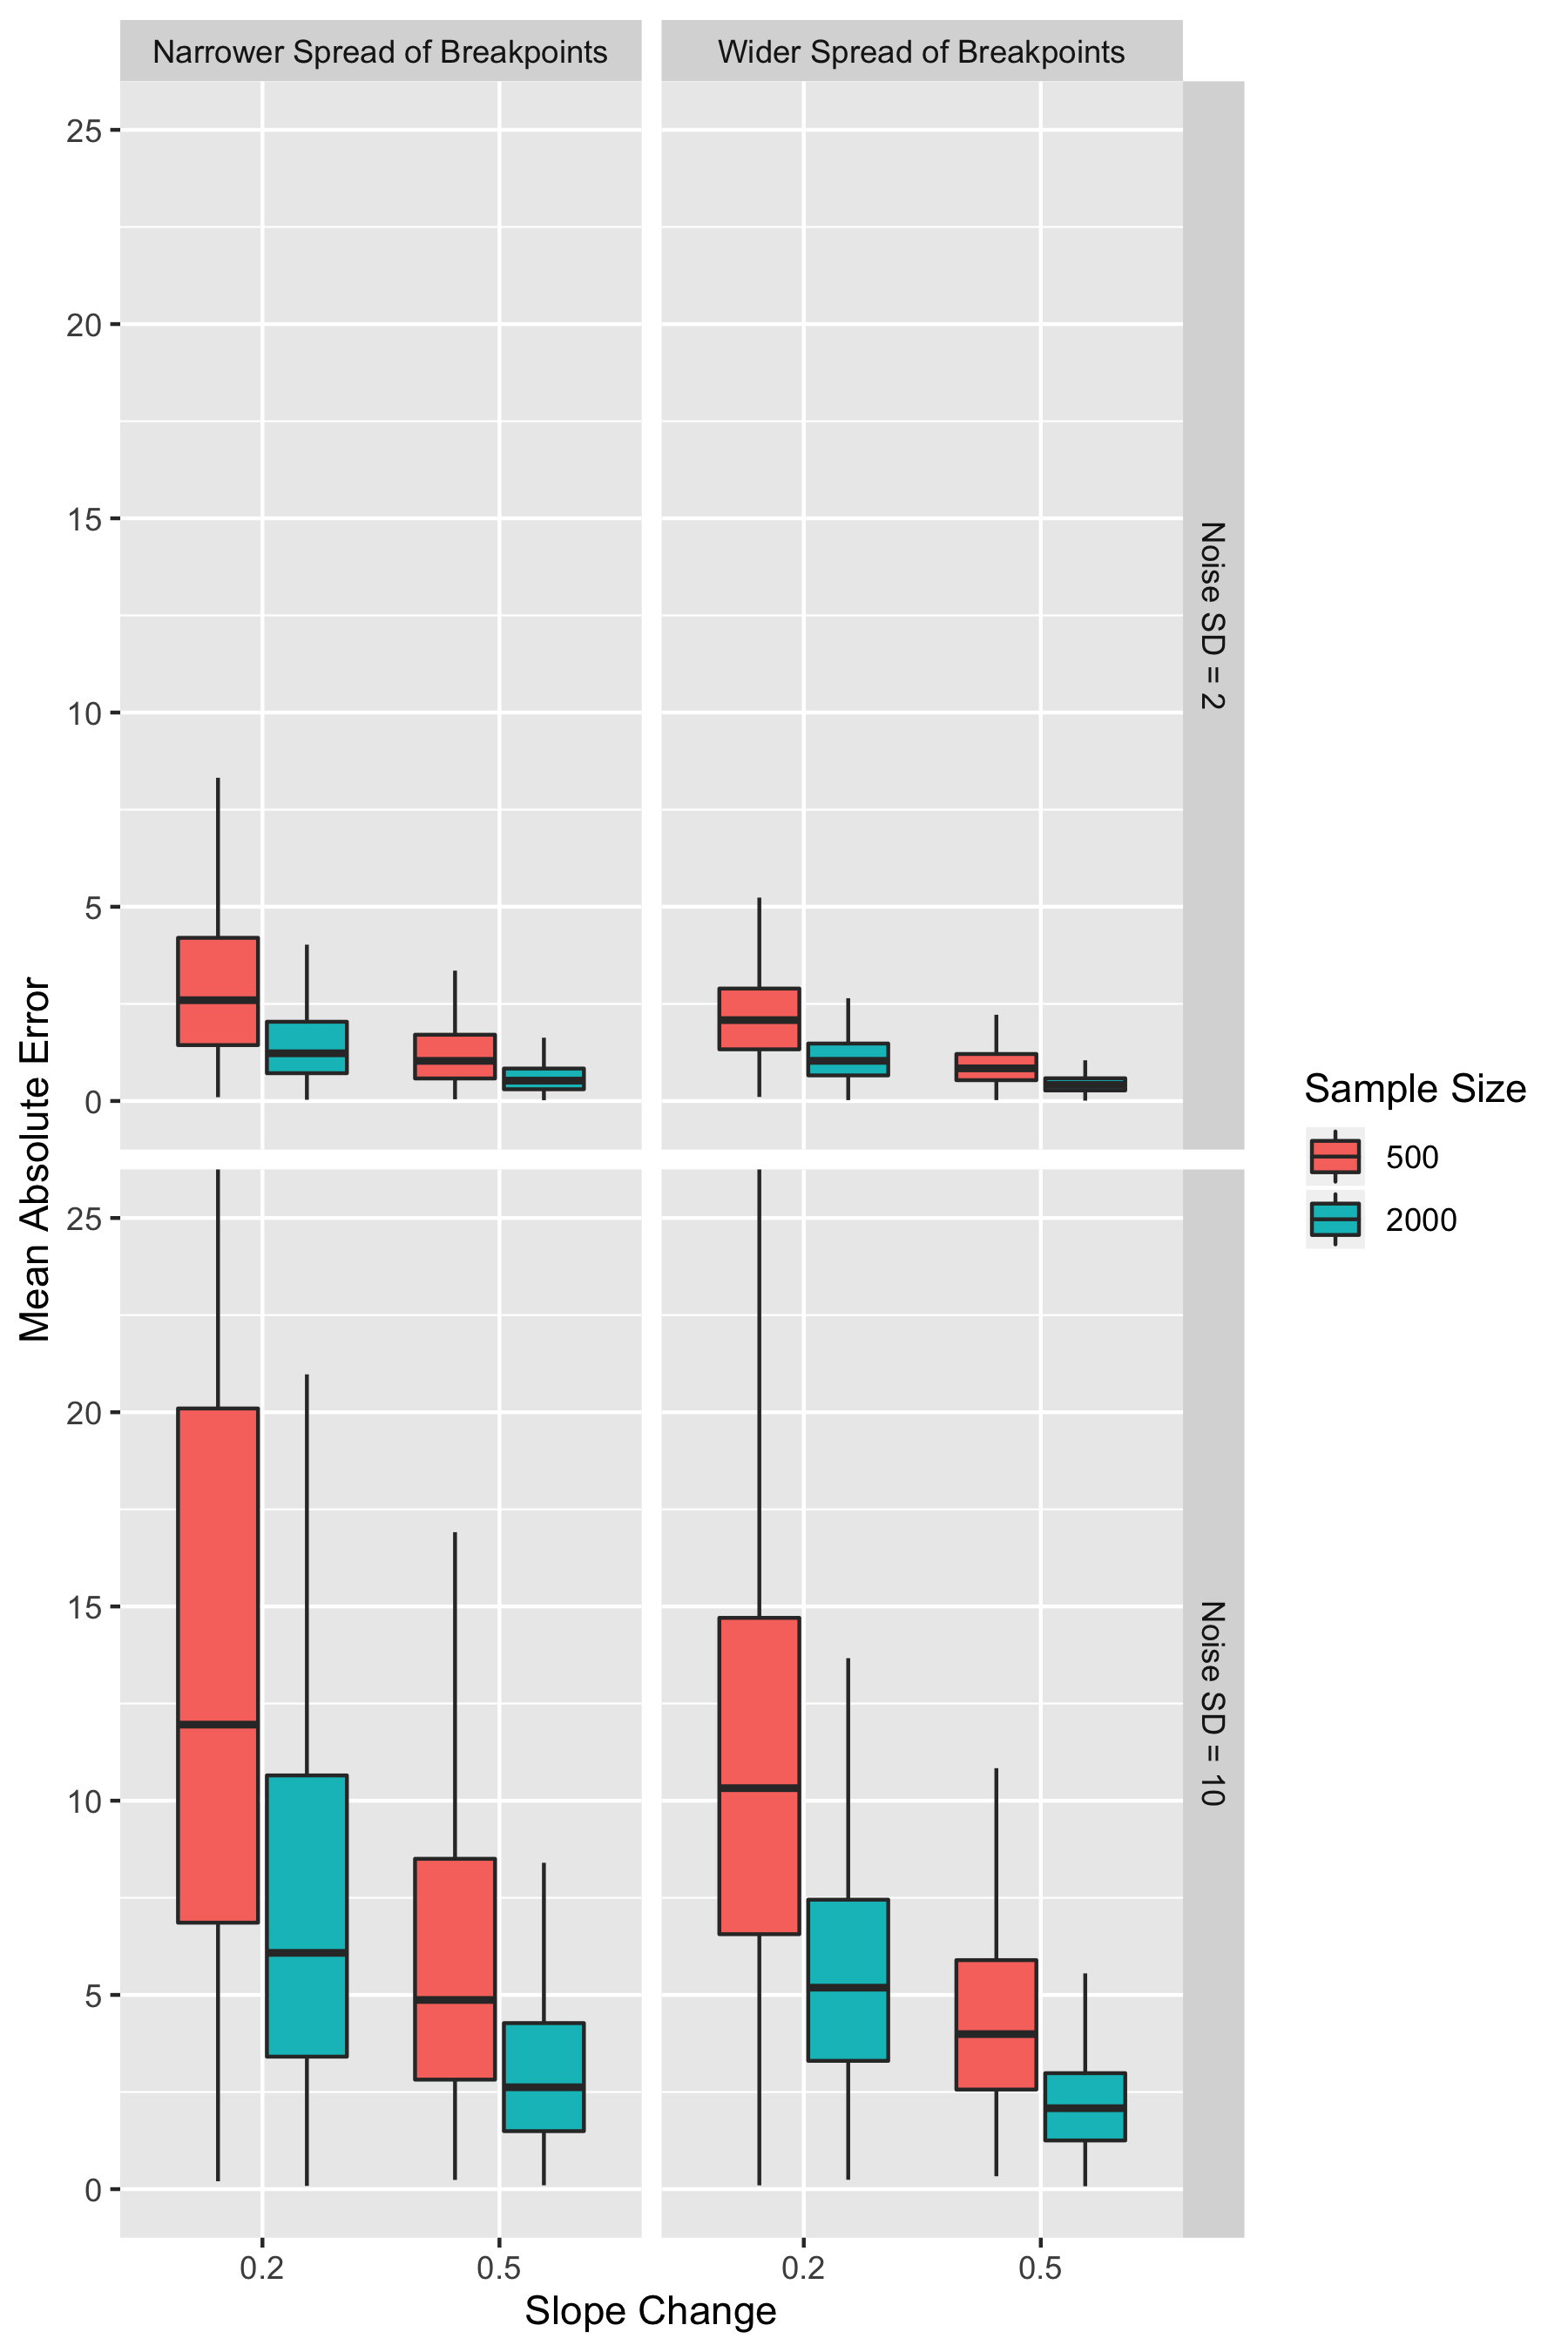
\includegraphics[width = 5.5 in]{Plot4_3.png}
    \caption{Boxplots of Distribution of Mean Absolute Error Based on 1,000 Replicates under Setting 3}
\end{figure}

Our estimation problem under Setting 3, with a continuous $Z$-covariate rather than a binary one, becomes even harder. Higher MAEs and RMSEs (compared to Settings 1 and 2) confirm this statement. Otherwise, the behavior of distributions for MAE and RMSE is similar to those under previous two settings.

\section{Setting 4: Covariate-specific Breakpoint and Slope Change with Continuous Covariates}
We generate data from the following model:
\begin{align*}
   y_i &= 0.2 x_i + (0.2 + \delta_{11} w_{1i}) (x_i - \psi_i)_+ + \epsilon_i \\
    \psi_i &= \dfrac{40 + 320 e^{\eta_i}}{1 + e^{\eta_i}} \\
    \eta_i &= z_{1i}
\end{align*}

where $x_i \sim U(40, 320), \epsilon_i \sim \mathcal{N}(0, \sigma^2)$ and $i = 1, 2, \cdots, N$. We set $N \in \{500, 2000\}$ and $\sigma \in \{2, 10\}$ as before. We set $z_{1i} \sim \mathcal{N}(0, k^2)$, and let $k \in \{0.5, 1.5\}$; that is, a larger $k$ value corresponds to a larger spread of breakpoint locations. Because $z_1$ is drawn from a continuous distribution in this setting, each observation will have its unique breakpoint unless two observations have identical $z_1$ values. Thus, to avoid imposing extra assumptions about the relationship between $x_i$'s and $\psi_i$'s, we use $\psi_i = \text{median}(x) - 10 = 170$ for all observations as an initial guess. Furthermore, we set $w_{1i} \sim \mathcal{N}(0, 1)$ and let $\delta_{11} \in \{0.1, 0.4\}$. In Table 4.4 and Figure 4.4, we present distributions of mean absolute error based on 1,000 replications of each possible combination of parameters noted above.

It is worth mentioning that the simulation results under this setting are not directly comparable to those under Settings 1-3, as we are no longer estimating a single slope parameter for every observation. Nevertheless, we observe similar patterns in the relationship between MAE/RMSE and $k, \sigma$, and $N$ compared to those of previous settings.

\begin{table}
\centering
\renewcommand\arraystretch{0.75}
\begin{tabular}{@{} lccccccccccc @{}} 
\toprule
    {Slope Change} & {$k$} & $\sigma$ & $N$ & \multicolumn{4}{c}{Sampling Distribution of} & \multicolumn{4}{c}{Sampling Distribution of} \\
    & & & & \multicolumn{4}{c}{MAE, $\mathbb{E}[\lvert \Hat{\psi_i} - \psi_i \rvert]$} & \multicolumn{4}{c}{RMSE, $\sqrt{\mathbb{E}[(\Hat{\psi_i} - \psi_i)^2]}$}\\
    \cmidrule(lr){5-8} \cmidrule(lr){9-12}
     & & & & Mean & Median & Q1 & Q3 & Mean & Median & Q1 & Q3 \\
\midrule
    $\delta_1 \sim \mathcal{N}(0.2, 0.1^2)$ & 0.5 & 2 & 500 & 1.98 & 1.64 & 1.00 & 2.64 & 2.12 & 1.80 & 1.15 & 2.75 \\
                     &     &   & 2000 & 0.99 & 0.82 & 0.50 & 1.34 & 1.05 & 0.94 & 0.56 & 1.42  \\
                     &     & 10 & 500 & 10.34 & 8.56 & 5.06 & 13.89 & 11.11 & 9.45 & 5.61 & 14.81 \\
                     &     &    & 2000 & 4.87 & 4.16 & 2.53 & 6.48 & 5.22 & 4.53 & 2.87 & 6.86 \\
                     & 1.5 & 2 & 500 & 1.74 & 1.58 & 1.06 & 2.28 & 1.96 & 1.80 & 1.19 & 2.56 \\
                     &     &   & 2000 & 0.85 & 0.76 & 0.53 & 1.13 & 0.95 & 0.88 & 0.60 & 1.26 \\
                     &     & 10 & 500 & 8.82 & 8.11 & 5.25 & 11.77 & 9.93 & 9.07 & 5.92 & 13.17 \\
                     &     &    & 2000 & 4.28 & 3.95 & 2.57 & 5.60 & 4.82 & 4.42 & 2.91 & 6.36 \\
\midrule
    $\delta_1 \sim \mathcal{N}(0.2, 0.4^2)$ & 0.5 & 2 & 500 & 0.75 & 0.63 & 0.38 & 1.01 & 0.81 & 0.71 & 0.43 & 1.07  \\
                     &     &   & 2000 & 0.35 & 0.31 & 0.19 & 0.47 & 0.38 & 0.34 & 0.22 & 0.51 \\
                     &     & 10 & 500 & 3.70 & 3.15 & 1.91 & 4.88 & 4.02 & 3.55 & 2.15 & 5.28 \\
                     &     &     & 2000 & 1.74 & 1.49 & 0.95 & 2.29 & 1.89 & 1.67 & 1.09 & 2.50 \\
                     & 1.5 & 2 & 500 & 0.74 & 0.69 & 0.42 & 0.95 & 0.84 & 0.77 & 0.47 & 1.09 \\
                     &     &     & 2000 & 0.36 & 0.33 & 0.20 & 0.47 & 0.40 & 0.36 & 0.23 & 0.53 \\
                     &     & 10 & 500 & 3.75 & 3.52 & 2.07 & 4.99 & 4.23 & 3.96 & 2.33 & 5.64 \\
                     &     &     & 2000 & 1.78 & 1.61 & 1.01 & 2.39 & 2.00 & 1.81 & 1.15 & 2.67 \\    
\bottomrule
\end{tabular}
\caption{Distribution of Mean Absolute Error and Root Mean Squared Error Based on 1,000 Replicates under Setting 4}
\end{table}

\begin{figure}
    \centering
    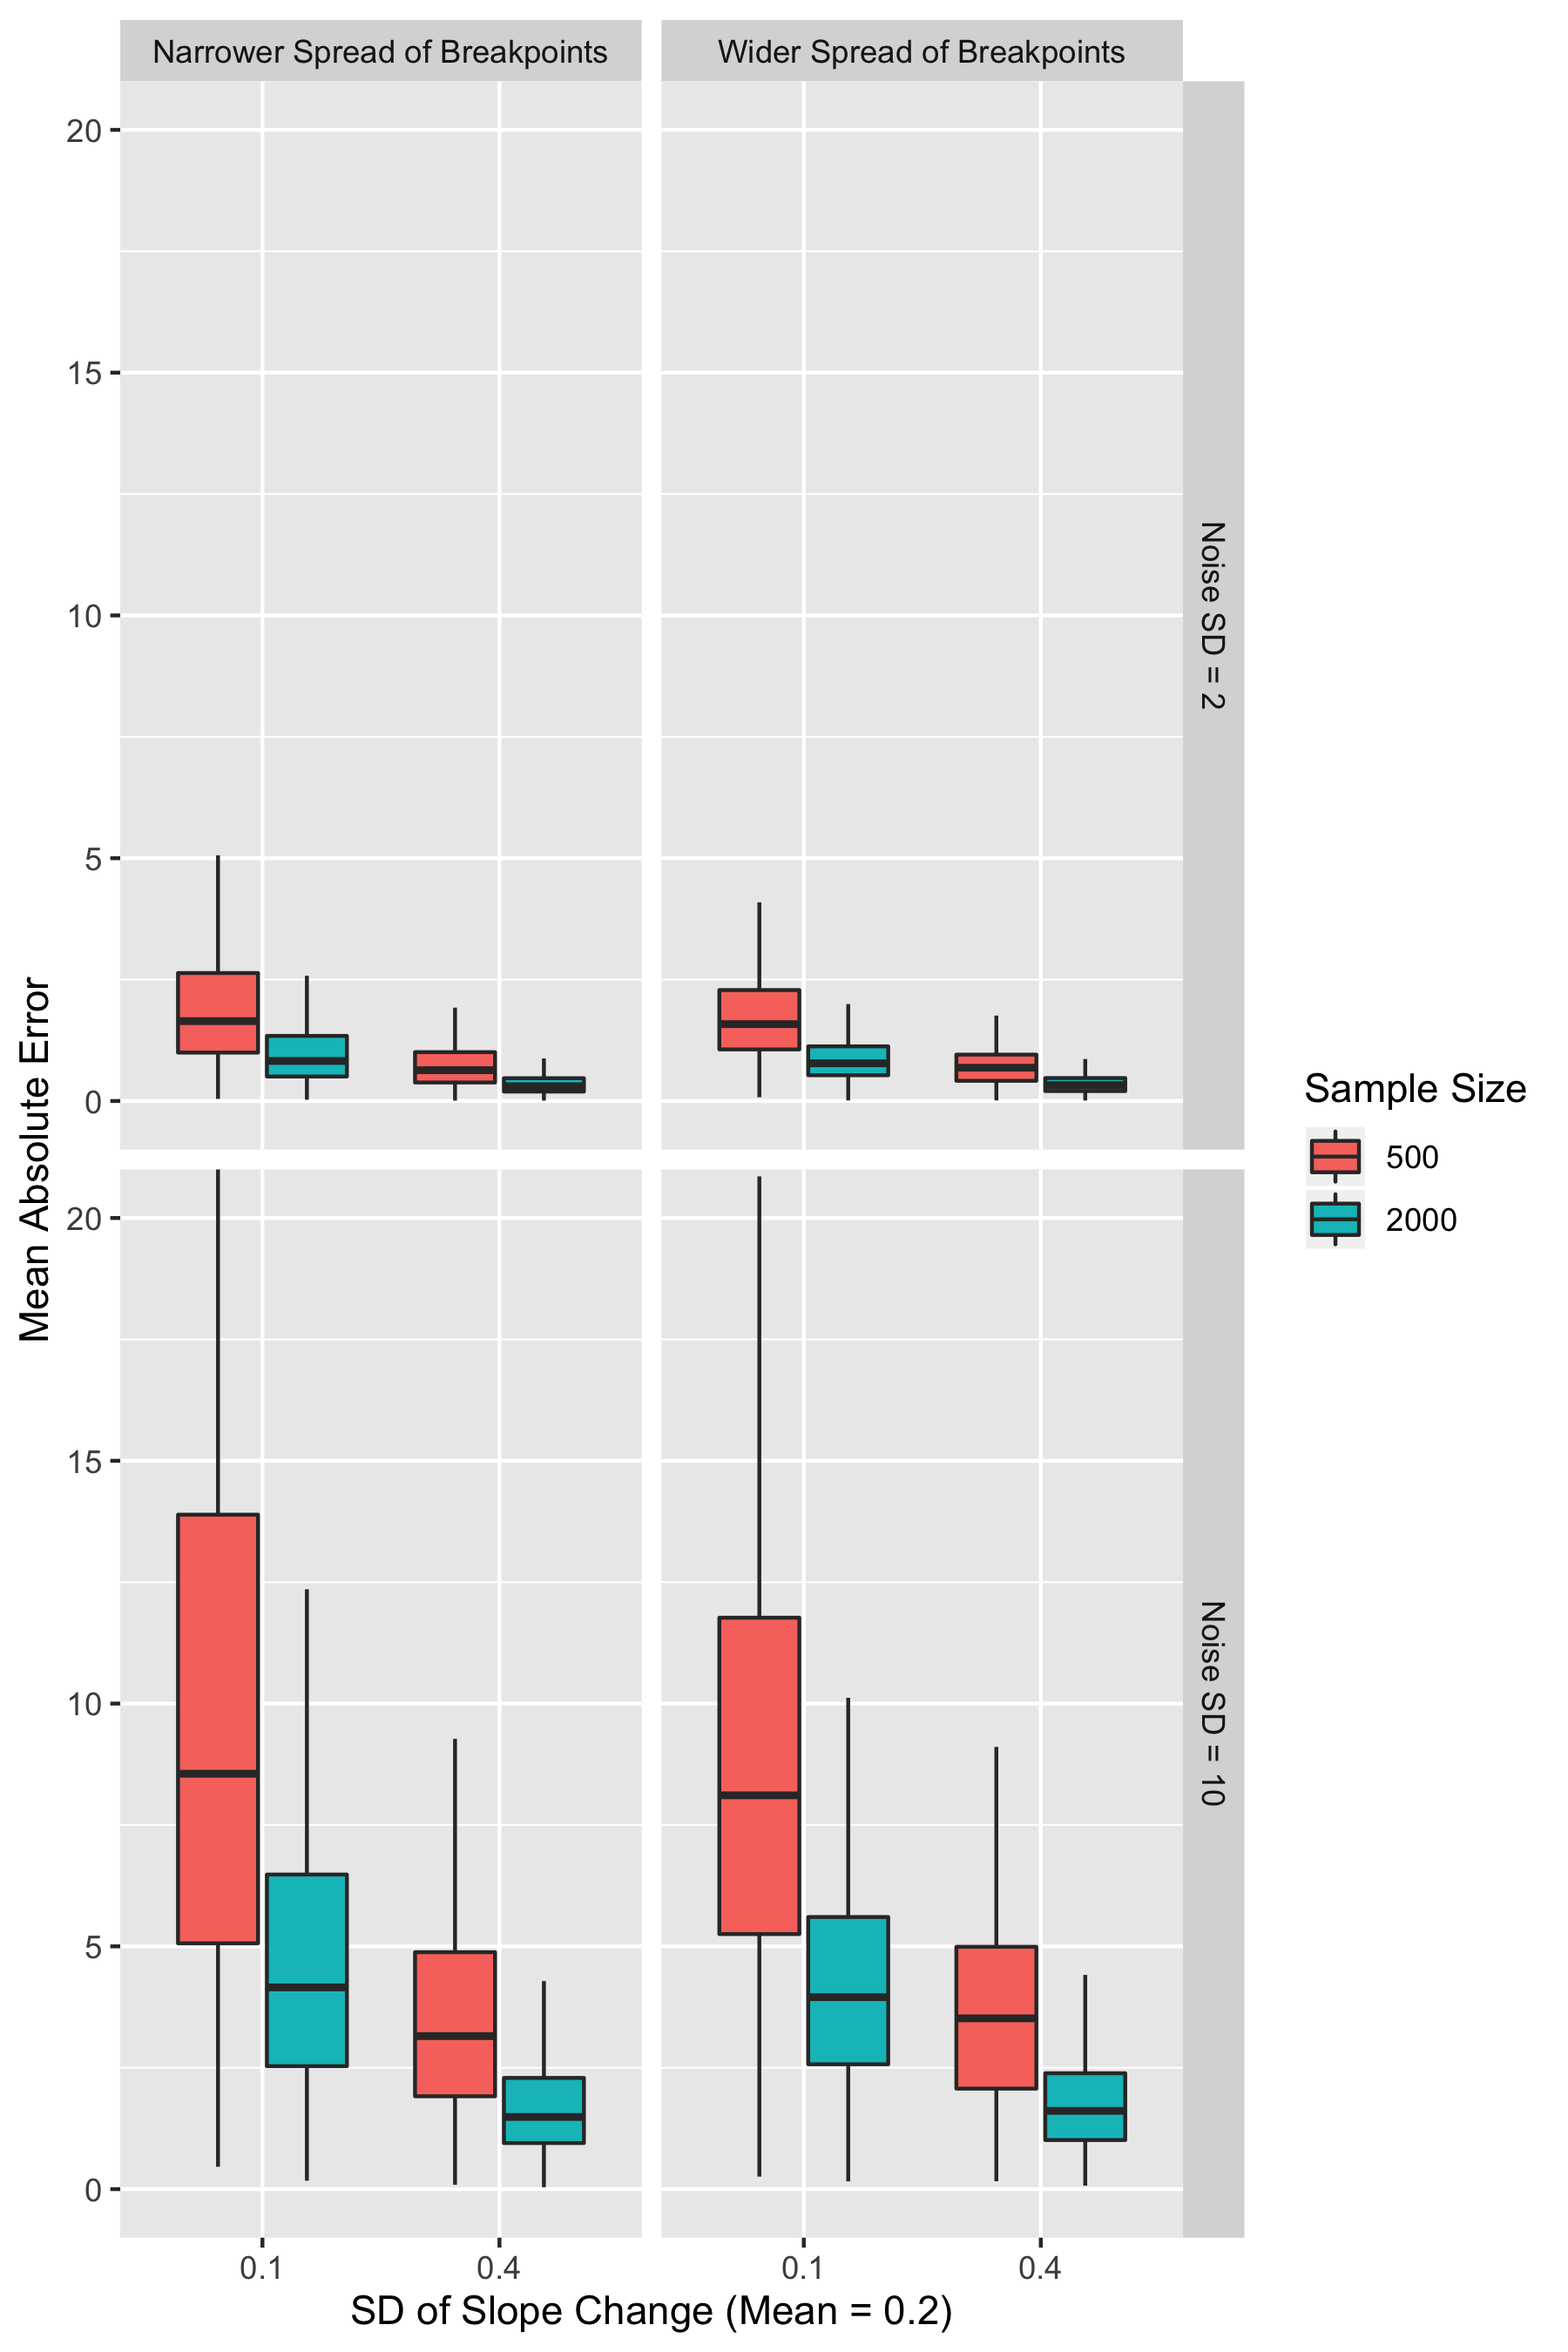
\includegraphics[width = 5.5 in]{Plot4_4.png}
    \caption{Boxplots of Distribution of Mean Absolute Error Based on 1,000 Replicates under Setting 4}
\end{figure}

\section{Some Remarks}
From Tables 4.1-4.4, we conclude that the methods in Chapter 3 performed reasonably well in all but the most challenging cases. To emulate our real-world data example in Chapter 5, we have consistently used a uniform distribution, $U(40, 320)$, to generate our main predictor of interest, $X$. In a large majority of cases in each setting, the means of both mean absolute error (MAE) and root mean squared error (RMSE) based on 1,000 iterations are no more than 5; in many cases where the slope change after the breakpoints are more pronounced (e.g. when $\delta_1 = 0.5$), means of both MAE and RMSE are less than 1.

We contend without proving that our estimator $\Hat{\psi}$ is $\sqrt{n}$-consistent; we empirically observe that quadrupling of the sample size leads to near halving of the mean for RMSE in every setting. Furthermore, slope changes are inversely related to MAE and RMSE, and standard deviations of the random noise are approximately linearly associated with MAE and RMSE. For settings 2 and 3, we also observe that a bigger spread of the breakpoint locations is associated with lower MAE and RMSE values by comparing cases with $k = 1.5$ and their counterparts with $k = 0.5$.

The complexity of the estimation problem increases as we move from Setting 1 (one breakpoint for all observations) to Setting 3 (one-to-one correspondence of $Z$-covariates and breakpoints). This is reflected in the distributions of MAE and RMSE; Given a combination of $\delta_1, \sigma$, and $N$, the means, medians, 1st quartile values, and 3rd quartile values of MAE and RMSE increase from Setting 1 to Setting 3.

In Setting 4, the addition of a continuous $W$-covariate in the slope parameter allows the slope change after the breakpoint to vary across different observations, and we observe that a larger spread of slope changes is associated with lower MAE and RMSE values, which is anticipated.

The algorithm converged within 20 iterations under all but the most challenging circumstances in all of the settings, with 10 bootstrap samples at each iteration. Nevertheless, non-convergence could still occur when the signal-to-noise ratio is low, or when the sample size is small.

% ========== Chapter 5

\chapter{An Application: Personalized Evaluation of Left Ventricular Enlargement with MESA Data}
In this chapter, we apply the method illustrated in Chapter 3 to a dataset from the MESA study to evaluate left ventricular enlargement of the study subjects. 

The dataset consists of 4,954 study subjects with non-missing values of ASCVD score, death, and left ventricular mass measured via cardiac MRI. ASCVD score is a measure co-developed by American College of Cardiology (ACC) and American Heart Association (AHA) that quantifies 10-year cumulative risks of atherosclerotic cardiovascular diseases (ASCVD) for patients aged 40 to 79. An individual's score is calculated using various demographic and clinical variable, including age, high-density and low-density lipoprotein levels, smoking status, and diabetes status \cite{ASCVD}. Race, gender, height, weight, body mass index (BMI) and body surface area (BSA) were also collected or computed for these study subjects. % See Table A.1 in Appendix A for a description of those variables of the MESA study subjects included in the analysis.

As discussed in Chapter 2.2, we postulate that for study subjects with the same gender and BMI, 10-year cardiovascular disease and mortality risks associated with having an enlarged left ventricle are higher after left ventricular mass exceeds a certain value. Thus, we treat ASCVD score and death as separate outcome variables and left ventricular mass as the primary predictor of interest. Since ASCVD scores predict 10-year risks of atherosclerotic cardiovascular diseases, we truncate our death outcome at 10 years (or 3,653 days) to ensure both outcome variables span the same time period. We then estimate covariate-specific breakpoints in the association between ASCVD score and left ventricular mass, as well as covariate-specific breakpoints in the association between 10-year truncated death and left ventricular mass, with gender and BMI as two ``$Z$-covariates'' in both cases. We further assume that slope changes at breakpoints are the same for all individuals, and do not include any ``$W$-covariates''.

\section{Covariate-specific Breakpoints in The Association between ASCVD Score and Left Ventricular Mass}

We first specify our model as follows:
\begin{align}
    y_i &= \beta_0 + \beta_1 x_i  + \delta_1 (x_i - \psi_i)_+ + \gamma_2 z_{2i} + \epsilon_i \\
    \psi_i &= \dfrac{a_1 + a_2 e^{\eta_i}}{1 + e^{\eta_i}} \\
    \eta_i &= \kappa_0 + \kappa_1 z_{1i} + \kappa_2 z_{2i}
\end{align}
where $y_i$ is defined as the calculated ASCVD score of subject $i$, $x_i$ is defined as left ventricular masses of subject $i$ (in grams), and $z_{1i}$ is defined as the body mass index of subject $i$ (in $kg \cdot m^{-2}$), respectively. Furthermore, we define $z_{2i} = 1$ if subject $i$ is male, and $z_{2i} = 0$ if otherwise. We assume that $\epsilon_i \sim \mathcal{N}(0, \sigma^2)$ as before. We include a term for gender in Equation (5.1) to adjust for effect of gender on ASCVD score, and treat $\gamma_2$ as a nuisance parameter. 

After removing outliers in left ventricular mass (2 males and 1 female), left ventricular masses of the participants range from 48.45 grams to 317.02 grams. Therefore, we set $[a_1, a_2] = [48.45, 317.02]$. Based on locally estimated scatterplot smoothing (LOESS) curves of ASCVD score versus left ventricular mass for both genders (Figure A.1, Appendix A), we choose $\psi_i^{(0)} = 120$ for females and $\psi_i^{(0)} = 180$ for males as initial guesses. The fitting algorithm achieved convergence within 20 iterations, with 10 bootstrap samples at each iteration. The total running time of the algorithm is less than 10 seconds.

We plot estimated breakpoint values in left ventricular mass, as well as their 90\% bootstrapped confidence intervals, as a function of BMI and gender below in Figure 5.1, and include Table 5.1 with numerical values of estimated breakpoint values for both genders at various body mass indices. ``NA'' in Table 5.1 indicates that breakpoint values cannot be estimated, as none of the males in the study cohort have a BMI of 44.0 or greater. We provide point estimates and 90\% bootstrapped confidence intervals of parameters $\kappa_0, \kappa_1$ and $\kappa_2$ in Table 5.2. Kernel density estimators of bootstrap distributions of $\kappa$ parameters are also provided in the Appendix (Figure A.7, Appendix A).

\begin{figure}
    \centering
    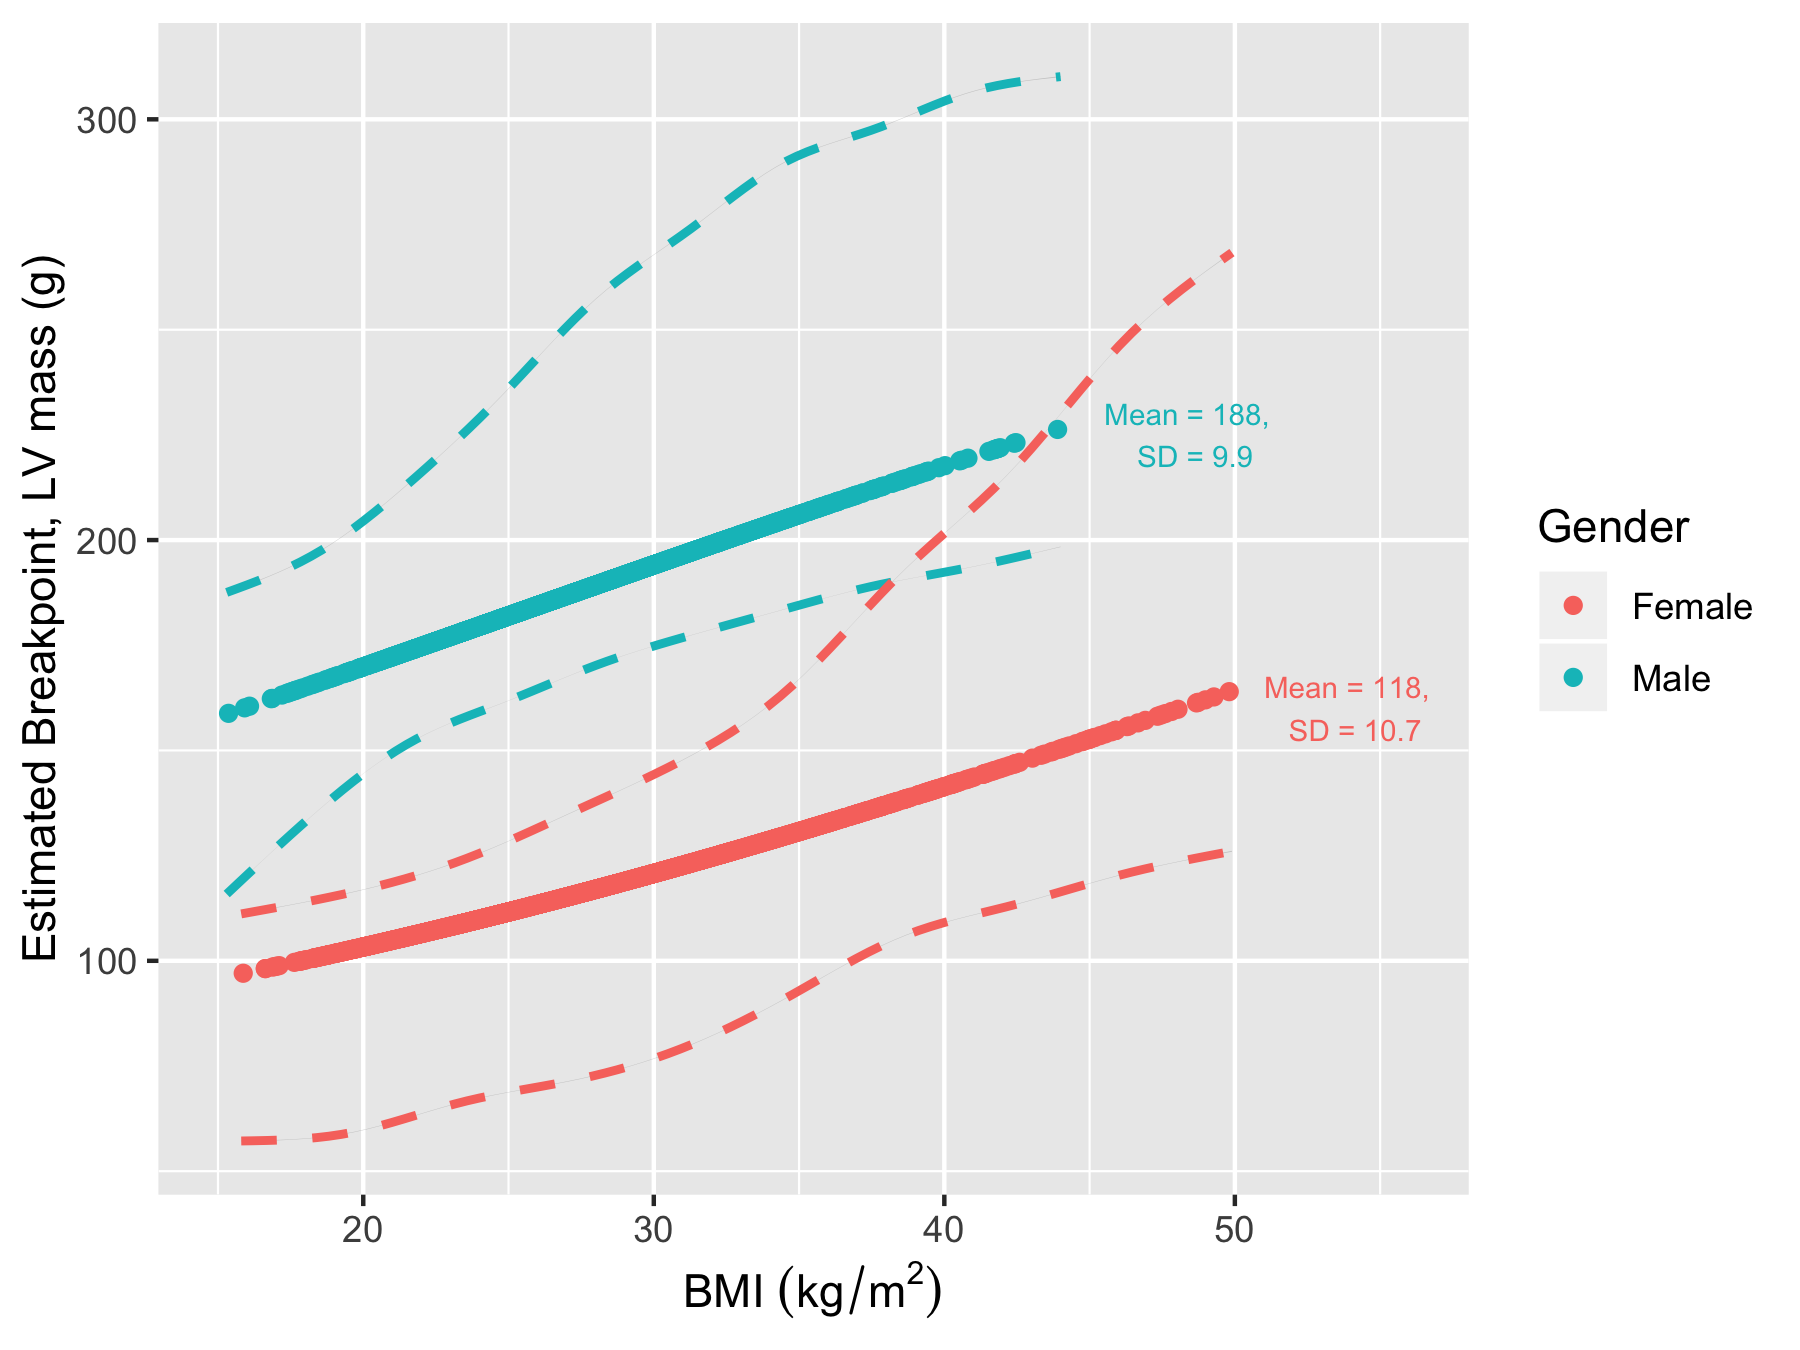
\includegraphics[width = 6 in]{Plot5_1.png}
    \caption{Estimated breakpoint values in LV mass and corresponding bootstrapped 90\% CIs as a function of BMI and gender with ASCVD score as outcome}
\end{figure}

\begin{table}
\centering
\renewcommand\arraystretch{0.75}
\begin{tabular}{@{} lcccccc @{}} 
\toprule
    {BMI Category} & {BMI ($kg \cdot m^{-2}$)} & \multicolumn{2}{c}{Estimated Breakpoints, $\Hat{\psi}_i$, and} \\
    & & \multicolumn{2}{c}{90\% bootstrapped CI ($g$)} \\
    \cmidrule(lr){3-4}
     & & Male & Female \\
\midrule
    Underweight & 17.0 & 162.7 (126.3, 192.2) & 98.7 (57.7, 112.7)\\
    & 18.5 & 166.3 (135.7, 196.7) & 101.0 (58.4, 114.6) \\
\midrule
    Normal & 20.0 & 169.9 (144.7, 204.5) & 103.3 (59.6, 117.0) \\
    & 21.5 & 173.5 (151.3, 212.7) & 105.7 (62.4, 119.6) \\
    & 23.0 & 177.1 (156.1, 222.7) & 108.2 (65.6, 122.5) \\
    & 24.5 & 180.8 (160.5, 232.6) & 110.7 (68.4, 127.1) \\
\midrule
    Overweight & 26.0 & 184.4 (164.7, 243.3) & 113.4 (70.3, 131.9) \\
    & 27.5 & 188.1 (168.8, 253.1) & 116.1 (71.8, 135.9) \\
    & 29.0 & 191.7 (172.6, 264.9) & 118.9 (74.0, 140.9) \\
\midrule
    Class 1 Obese & 30.5 & 195.3 (175.8, 270.2) & 121.7 (79.4, 146.0) \\
    & 32.0 & 198.9 (178.8, 277.1) & 124.7 (82.5, 151.8) \\
    & 33.5 & 202.5 (181.8, 285.6) & 127.7 (85.7, 157.4) \\
\midrule
    Class 2 Obese & 35.0 & 206.1 (184.4, 291.2) & 130.7 (92.9, 168.1) \\
    & 36.5 & 209.6 (177.4, 295.0) & 133.8 (100.0, 177.3) \\
    & 38.0 & 213.0 (189.7, 298.9) & 137.1 (104.4, 188.2) \\
    & 39.5 & 216.5 (191.8, 302.5) & 140.3 (107.6, 198.8) \\
\midrule
    Class 3 Obese & 41.0 & 219.8 (193.6, 306.7) & 143.7 (110.3, 208.5) \\
    & 42.5 & 223.2 (196.0, 308.9) & 147.0 (113.9, 218.5) \\
    & 44.0 & NA & 150.5 (116.9, 230.1) \\
    & 45.5 & NA & 153.9 (119.5, 242.9) \\
    & 47.0 & NA & 157.2 (121.4, 252.6) \\
\bottomrule
\end{tabular}
\caption{Estimated breakpoint values in LV mass and corresponding bootstrapped 90\% CIs, by gender and BMI, with ASCVD score as outcome}
\end{table}

\begin{table}
\centering
\renewcommand\arraystretch{0.75}
\begin{tabular}{@{} lcc @{}} 
\toprule
    {Parameter} & {Point Estimate} & {90\% Bootstrapped CI} \\
\midrule
    $\kappa_0$ & $-2.08$ & $(-5.59, -1.55)$ \\
    $\kappa_1$ & $0.0362$ & $(0.0184, 0.127)$ \\
    $\kappa_2$ & $1.17$ & $(0.949, 3.00)$ \\
\bottomrule
\end{tabular}
\caption{Estimated $\kappa$ parameters and corresponding bootstrapped 90\% CIs, with ASCVD score as outcome}
\end{table}

Our results are easy to interpret: for example, given a BMI of 35 $kg/m^2$, we estimate that rate of change in 10-year ASCVD score per unit difference in BMI is higher if the LV mass is greater than 206.1 grams for men and 130.7 grams for women. We also observe that for both genders, the estimated breakpoint values are higher at higher left ventricular masses. However, gender has a considerable effect on the breakpoint location: Compared with females with the same BMI value, in this dataset males have fitted breakpoint values in left ventricular mass that are higher by 64 to 76 grams depending on the actual BMI value. This difference in fitted breakpoint values is statistically significant, as the 90\% bootstrapped confidence interval for $\kappa_2$ does not include 0. This is likely due to adult males having clinically and statistically significantly higher left ventricular mass than adult females after adjusting for body size measures such as weight and BMI \cite{GdS1995, CS2002}.

\section{Covariate-specific Breakpoints in The Association between 10-Year Truncated Death and Left Ventricular Mass}

Similar to what we did in Chapter 5.1, we first define the model as follows:
\begin{align}
    \text{logit}(\mathbb{E}[y_i]) &= \beta_0 + \beta_1 x_i + \delta_1 (x_i - \psi_i)_+ + \gamma_2 z_{2i} \\
    \psi_i &= \dfrac{a_1 + a_2 e^{\eta_i}}{1 + e^{\eta_i}} \\
    \eta_i &= \kappa_0 + \kappa_1 z_{1i} + \kappa_2 z_{2i}
\end{align}

where $y_i = 1$ if subject $i$ died no later than 10 years (3,653 days) since the start of the study period and $y_i = 0$ otherwise. $x_i$ is defined as left ventricular mass of subject $i$ (in grams), and $z_{1i}$ is defined as the body mass index of subject $i$ (in $kg \cdot m^{-2}$), respectively.  Furthermore, we define $z_{2i} = 1$ if subject $i$ is male, and $z_{2i} = 0$ if otherwise. We include a term in Equation (5.4) to account for the effect of gender on 10-year all-cause mortality, treat $\gamma_2$ as a nuisance paramenter, and set $[a_1, a_2] = [48.45, 317.02]$ as we did in Chapter 5.1. Based on LOESS curves of 10-year all-cause mortality versus left ventricular mass for both genders (Figure A.2, Appendix A), we choose $\psi_i^{(0)} = 135$ for females and $\psi_i^{(0)} = 165$ for males as initial guesses.

We plot estimated breakpoint values in left ventricular mass, as well as their 90\% bootstrapped confidence intervals, as a function of BMI and gender above in Figure 5.2, and include Table 5.3 with numerical values of estimated breakpoint values for both genders at various body mass indices. ``NA'' in Table 5.3 indicates that breakpoint values cannot be estimated, as none of the males in the study cohort has a BMI of 44.0 or greater. We provide point estimates and 90\% bootstrapped confidence intervals of $\kappa_0, \kappa_1$ and $\kappa_2$ in Table 5.4. Kernel density estimators of bootstrap distributions of $\kappa$ parameters are also provided in the Appendix (Figure A.8, Appendix A).

\begin{figure}
    \centering
    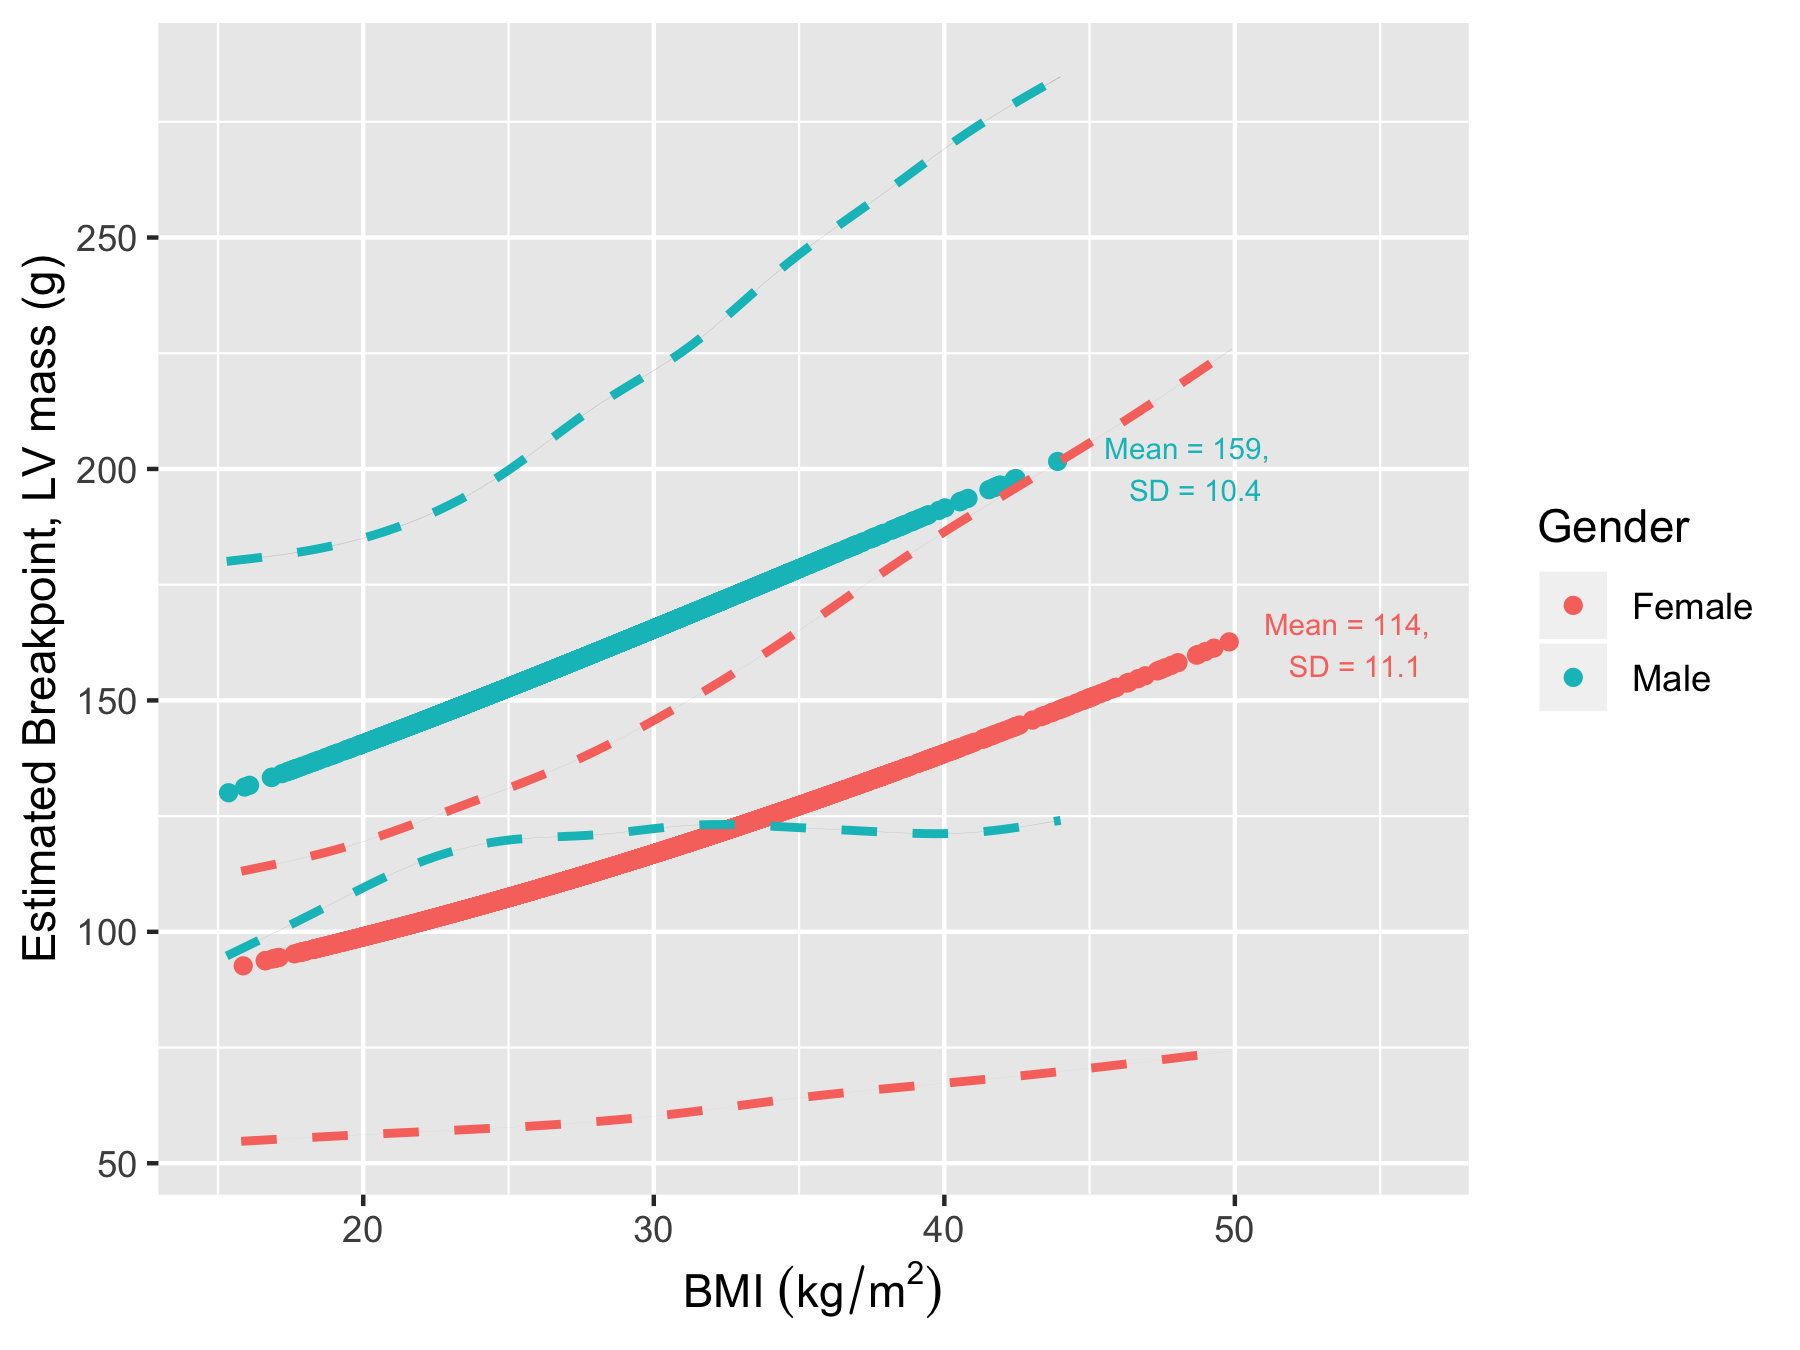
\includegraphics[width = 6 in]{Plot5_2.png}
    \caption{Estimated breakpoint values in LV mass and corresponding bootstrapped 90\% CIs as a function of BMI and gender with 10-year truncated death as outcome}
\end{figure}

\begin{table}
\centering
\renewcommand\arraystretch{0.75}
\begin{tabular}{@{} lcccccc @{}} 
\toprule
    {BMI Category} & {BMI ($kg \cdot m^{-2}$)} & \multicolumn{2}{c}{Estimated Breakpoints, $\Hat{\psi}_i$, and} \\
    & & \multicolumn{2}{c}{90\% bootstrapped CI ($g$)} \\
    \cmidrule(lr){3-4}
     & & Male & Female \\
\midrule
    Underweight & 17.0 & 148.9 (99.6, 181.6) & 102.4 (55.2, 114.2)\\ 
    & 18.5 & 152.5 (104.3, 183.6) & 104.8 (55.7, 116.5) \\
\midrule
    Normal & 20.0 & 156.2 (110.2, 184.6) & 107.4 (56.2, 119.8) \\
    & 21.5 & 159.8 (114.5, 189.2) & 110.0 (56.6, 122.9) \\
    & 23.0 & 163.6 (116.4, 192.5) & 112.8 (57.1, 126.3) \\
    & 24.5 & 167.3 (119.5, 196.9) & 115.6 (57.7, 129.8) \\
\midrule
    Overweight & 26.0 & 171.1 (120.4, 202.2) & 118.5 (58.1, 133.3) \\
    & 27.5 & 174.6 (120.9, 211.9) & 121.5 (58.7, 137.9) \\
    & 29.0 & 178.7 (121.3, 216.3) & 124.5 (59.5, 142.8) \\
\midrule
    Class 1 Obese & 30.5 & 182.5 (122.4, 222.7) & 127.6 (60.5, 147.3) \\
    & 32.0 & 186.3 (123.7, 231.4) & 130.8 (61.8, 152.7) \\
    & 33.5 & 190.1 (123.2, 237.2) & 134.1 (62.8, 158.4) \\
\midrule
    Class 2 Obese & 35.0 & 193.9 (122.5, 247.1) & 137.5 (64.4, 165.5) \\
    & 36.5 & 197.7 (121.6, 252.5) & 140.9 (65.0, 171.7) \\
    & 38.0 & 201.4 (121.2, 260.0) & 144.3 (66.1, 178.3) \\
    & 39.5 & 205.1 (121.4, 266.9) & 147.8 (67.1, 184.2) \\
\midrule
    Class 3 Obese & 41.0 & 208.8 (121.3, 273.7) & 151.5 (68.1, 190.2) \\
    & 42.5 & 212.4 (122.6, 279.5) & 155.0 (68.9, 196.6) \\
    & 44.0 & NA & 158.7 (69.8, 202.0) \\
    & 45.5 & NA & 162.4 (70.8, 207.5) \\
    & 47.0 & NA & 166.2 (72.2, 213.8) \\
\bottomrule
\end{tabular}
\caption{Estimated breakpoint values in LV mass and corresponding bootstrapped 90\% CIs, by gender and BMI, with 10-year truncated death as outcome}
\end{table}

\begin{table}
\centering
\renewcommand\arraystretch{0.75}
\begin{tabular}{@{} lcc @{}} 
\toprule
    {Parameter} & {Point Estimate} & {90\% Bootstrapped CI} \\
\midrule
    $\kappa_0$ & $-2.74$ & $(-5.65, -0.91)$ \\
    $\kappa_1$ & $0.0712$ & $(-0.00271, 0.105)$ \\
    $\kappa_2$ & $0.508$ & $(0.230, 3.54)$ \\
\bottomrule
\end{tabular}
\caption{Estimated $\kappa$ parameters and corresponding bootstrapped 90\% CIs, with 10-year truncated death as outcome}
\end{table}

Interpretation of the results is similar to that of Chapter 5.1: for example, given a subject with BMI of 35 $kg/m^2$, we estimate that 10-year risks of death begins to increase if the LV mass is greater than 193.9 grams for men and 137.5 grams for women. We observe that the estimated breakpoint values are lower for males and slightly lower for females compared to results from Figure 5.1 and Table 5.1. We again observe that for both genders, the estimated breakpoint values are higher at higher left ventricular masses, and a sizable effect of gender on breakpoint locations remains. This effect is statistically significant, as the 90\% bootstrapped confidence interval for $\kappa_2$ does not include 0.

\section{Some Remarks}

In this chapter, we are providing a more flexible and interpretable approach of estimating the left ventricular mass at which a larger heart begins to lead to increased ASCVD score or 10-year death risk for a given body size and gender. We achieve this by applying our method of fitting covariate-specific breakpoints outlined in Chapter 3.

It is evident that left ventricular mass is heavily dependent on gender as well as body size measures, such as height, weight, and body mass index. Therefore, for the purpose of evaluating left ventricular enlargement, it is essential to take gender and body size measures into consideration.

Our methodology incorporates body size and gender into the estimation directly whereas current methods mostly use pre-scaled versions of left ventricular mass (such as LVM/BSA, LVM/$h$, LVM/$h^{2.7}$). This leads to a more natural interpretation of the results because the estimated breakpoints are defined in the original measurement units (in this case, grams). It is also straightforward to incorporate additional covariates in the estimation of breakpoints as needed.

It is worth mentioning that bootstrap distributions of $\kappa$ parameters have heavy tails in both models (Figures A.7 and A.8, Appendix A). This relates to the identifiability of model parameters. We observe that if $\delta_1$ converges to zero (i.e. there is no breakpoint), then the $\kappa$ parameters are unidentifiable as the $\delta_1 (x_i - \psi_i)_+$ term also converges to zero. On the other hand, if $\kappa$ parameters have large absolute values, then the estimated $\psi_i$'s converge to either the minimum possible value $a_1$ or the maximum $a_2$, rendering the $\delta_1$ estimate irrelevant. Values in the heavy tails of bootstrap distribution of $\kappa$'s reflect model instances with these characteristics, which are possible, but unlikely, explanations of the relationship between estimated breakpoint in LV mass and BMI. Therefore, if the true relationship between the outcome and the predictor variables does not strongly support the existence of a breakpoint, the model may produce a fit containing $\kappa$ parameters with extremely high absolute values.

% ========== Chapter 6

\chapter{Discussion}

In this thesis, we described a simple and straightforward approach to estimate segmented regression models while enabling breakpoints to be determined by one or more covariates that may or may not be main predictors of interest (i.e. covariate-specific breakpoints). The obstacle of a non-linear term presenting in the model was overcome by performing a first-order Taylor expansion of the non-linear term around some initial guess followed by iteratively fitting models. 

Such an approach, originally developed by V. Muggeo \cite{VM2003, VM2014}, was inspired by our scientific interest of developing a personalized and flexible approach to evaluate the risks of left ventricular enlargement based on data from the MESA study, an ongoing, large-scale cohort study of cardiovascular diseases in the United States \cite{MESA}. This method serves two important purposes in the evaluation of left ventricular enlargement: it estimates a point at which the heart becomes sufficiently enlarged to start to affect a person's health, and it incorporates body size measures and gender in a flexible, easy-to-interpret way. By using this method, we can relax assumptions that the prevalence of having abnormally high LV mass is fixed at some number (for example, 5\%) in a healthy population.

A major advantage of the method is its flexibility while being highly interpretable. Estimating multiple breakpoints of the same variable and fitting multiple variables with breakpoints are both possible. Covariate-specific breakpoints could also be effectively estimated. Furthermore, alternative functions, such as a linear function, could be used to model the relationship between the breakpoint and breakpoint covariates (i.e. the $g(\cdot)$ function in Equation (3.9)), which provides an additional layer of flexibility. It is also possible to model the slope change after the breakpoint.

Furthermore, thanks to the linear approximation of the breakpoint term, the model could be fitted in the generalized linear model framework without requiring \textit{ad hoc} methods for estimation of breakpoint locations. As a result, it could be easily implemented with statistical software packages (\textit{e.g.} R, SAS, Python). This is an important advantage, because fitting non-linear models could be quite computationally expensive, especially with large sample sizes and/or additional explanatory variables. Currently, the R package ``segmented'', authored by V. Muggeo, is available; however, the package does not currently support estimation of covariate-specific breakpoints considered in Section 3.2 (as of version 1.2-0, June 23, 2020). For this thesis, an implementation was created in the R statistical language that enabled the estimation of both ``Covariate in Breakpoint Only'' and ``Covariates in Breakpoint and Slope'' models introduced in Sections 3.2.2 and 3.2.3 \cite{R}.

There are several items outside the scope of this thesis that merit some discussion. First of all, interval estimation of breakpoints, which provides a measure of uncertainty of the point estimates of the breakpoints, was not discussed in detail. Although we could use Taylor series expansion to approximate the non-linear breakpoint term, statistical inference about the likelihood function of model cannot be easily simplified accordingly. It has been shown that normal distribution based standard errors underestimate the actual variability of $\Hat{\psi}$, and therefore confidence intervals constructed using those standard errors are not recommended \cite{VM2017}. To address this problem, Muggeo introduced a smoothed score-based approach to interval estimation of breakpoints in segmented regression in 2017 \cite{VM2017}. An alternative way of obtaining reasonable $\alpha$\% confidence intervals of $\Hat{\psi}$ is creating bootstrap samples from the original sample and using the empirical ${\alpha/2}^{th}$ and $(100 - \alpha/2)^{th}$ percentiles of $\Hat{\psi}$ as the endpoints of the interval (i.e. nonparametric bootstrap).

It is worth mentioning that the success of algorithms introduced in this thesis depend on the existence of at least one breakpoint in the relationship between the outcome and the primary predictor of interest; otherwise, some model parameters might be unidentifiable, and our method could produce breakpoint parameter estimates with large and potentially nonsensical absolute values (as we saw in Chapter 5). Therefore, besides interval estimation, testing for the existence of breakpoint(s) is also of interest and currently represents an active research question. In the case with a common breakpoint for all observations (i.e. the model in Chapter 3.1), multiple authors have confirmed that the distribution of test statistics is complicated and dependent on the alternative hypothesis. Nevertheless, there are several methods to detect the existence of breakpoints, typically with the null hypothesis being 0 breakpoints exist in the relationship, and the alternative hypothesis being at least one breakpoint exists. 
On the other hand, there is scarce research on testing for existence of covariate-specific breakpoints introduced in the models in Chapter 3.2.

We observe that the performance of the estimator $\Hat{\psi}$ is sensitive to the initial guess supplied to the algorithm, $\psi^{(0)}$. This is a common issue for most non-convex estimation problems where the initial values for all paramenters have to be specified. In addition, estimation could be problematic when the signal-to-noise ratio is small, which often result in the concavity of the log-likelihood function and the existence of multiple local maxima. Regardless, the bootstrap restarting algorithm introduced in Chapter 3.2.4 proved to be an effective measure to escape local maxima when fitting the model iteratively.

Overall, we found the model to be quite promising: it is a flexible model that builds upon well-developed statistical methods and provides an estimator with satisfactory statistical properties, with straightforward interpretations for all parameters. As a result, we envision useful applications of the model in a variety of subject areas where estimating flexible and covariate-specific breakpoints is critical. The author of this thesis intends to port the algorithms illustrated in the thesis to Python 3.8.3 in the near future and publish the algorithm on GitHub.


%
% ==========   Bibliography
%
\nocite{*}   % include everything in the uwthesis.bib file
\bibliographystyle{plain}
\bibliography{uwthesis}
%
% ==========   Appendices
%
\appendix
\raggedbottom\sloppy

% ========== Appendix A
 
\chapter{Supplementary Figures}

This appendix contains supplementary figures for the thesis. Descriptions could be found in the main text and in the captions of these figures.

\begin{figure}
    \centering
    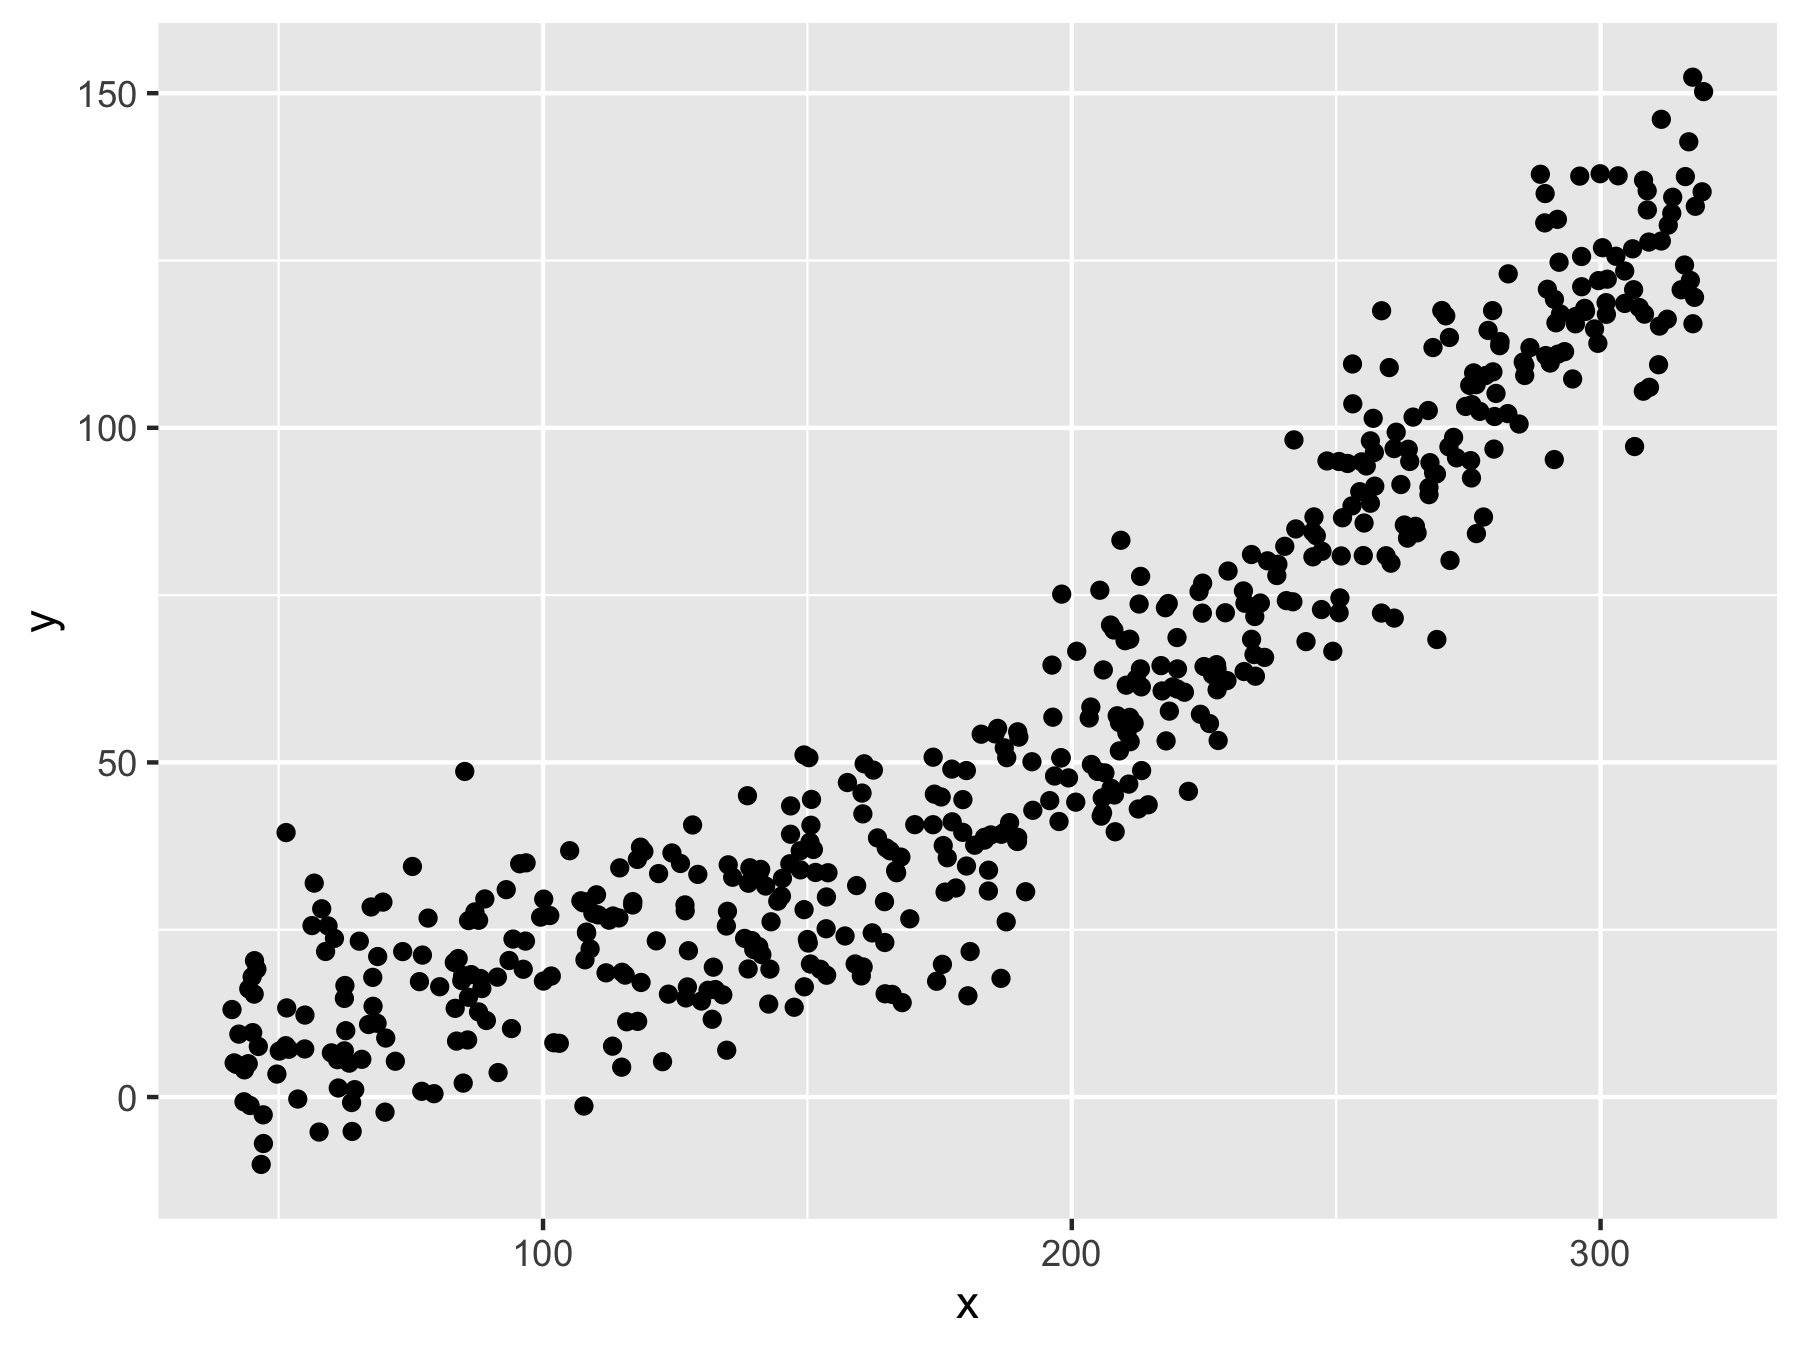
\includegraphics[width = 6 in]{PlotA_1.png}
    \caption{Example data generated under Setting 1 of simulation studies; $\psi = 180, N = 500, \delta_1 = 0.5, \sigma = 10$}
\end{figure}

\begin{figure}
    \centering
    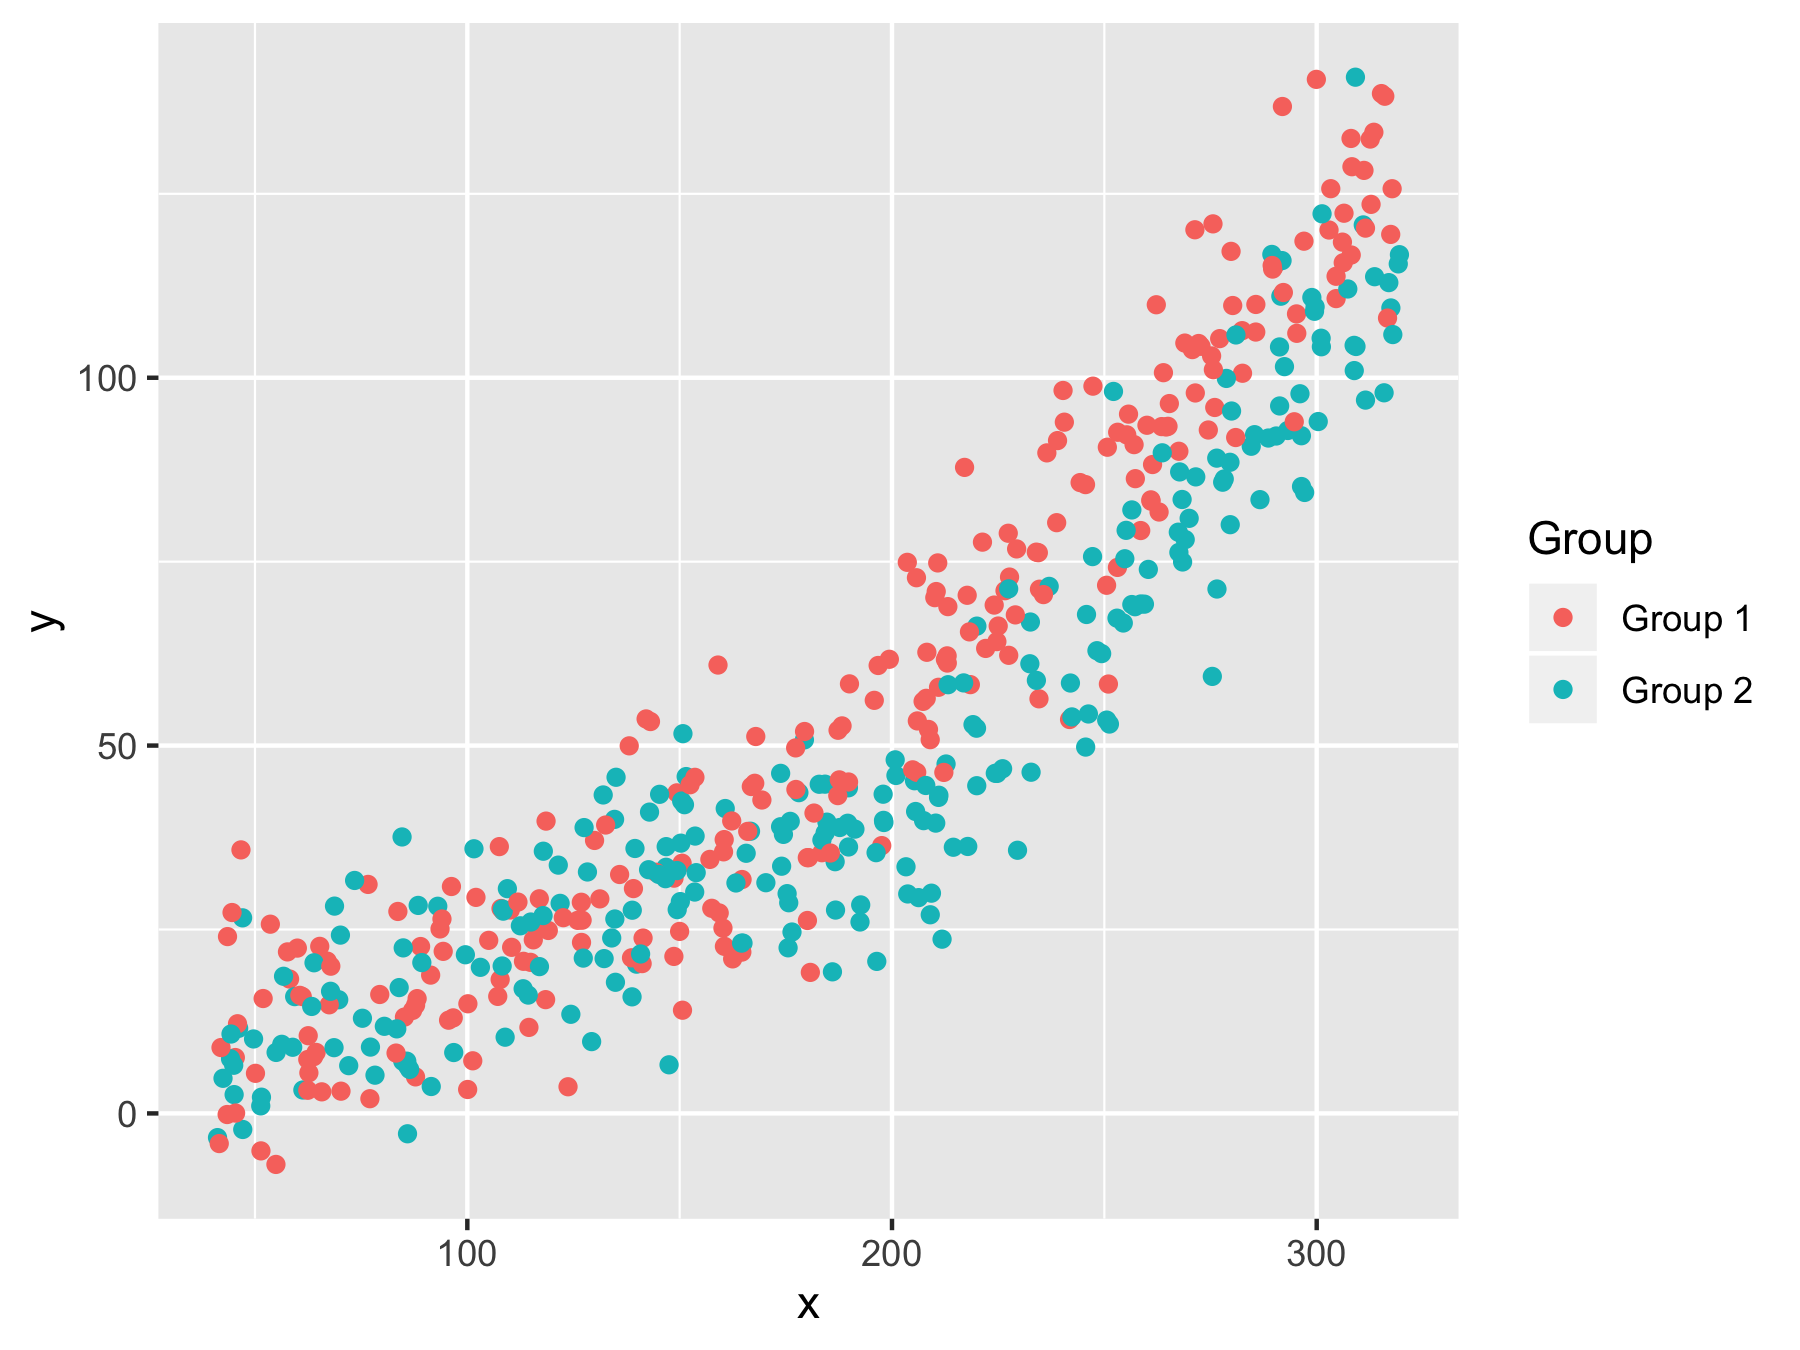
\includegraphics[width = 6 in]{PlotA_2.png}
    \caption{Example data generated under Setting 2 of simulation studies; $k = 0.5, N = 500, \delta_1 = 0.5, \sigma = 10$}
\end{figure}

\begin{figure}
    \centering
    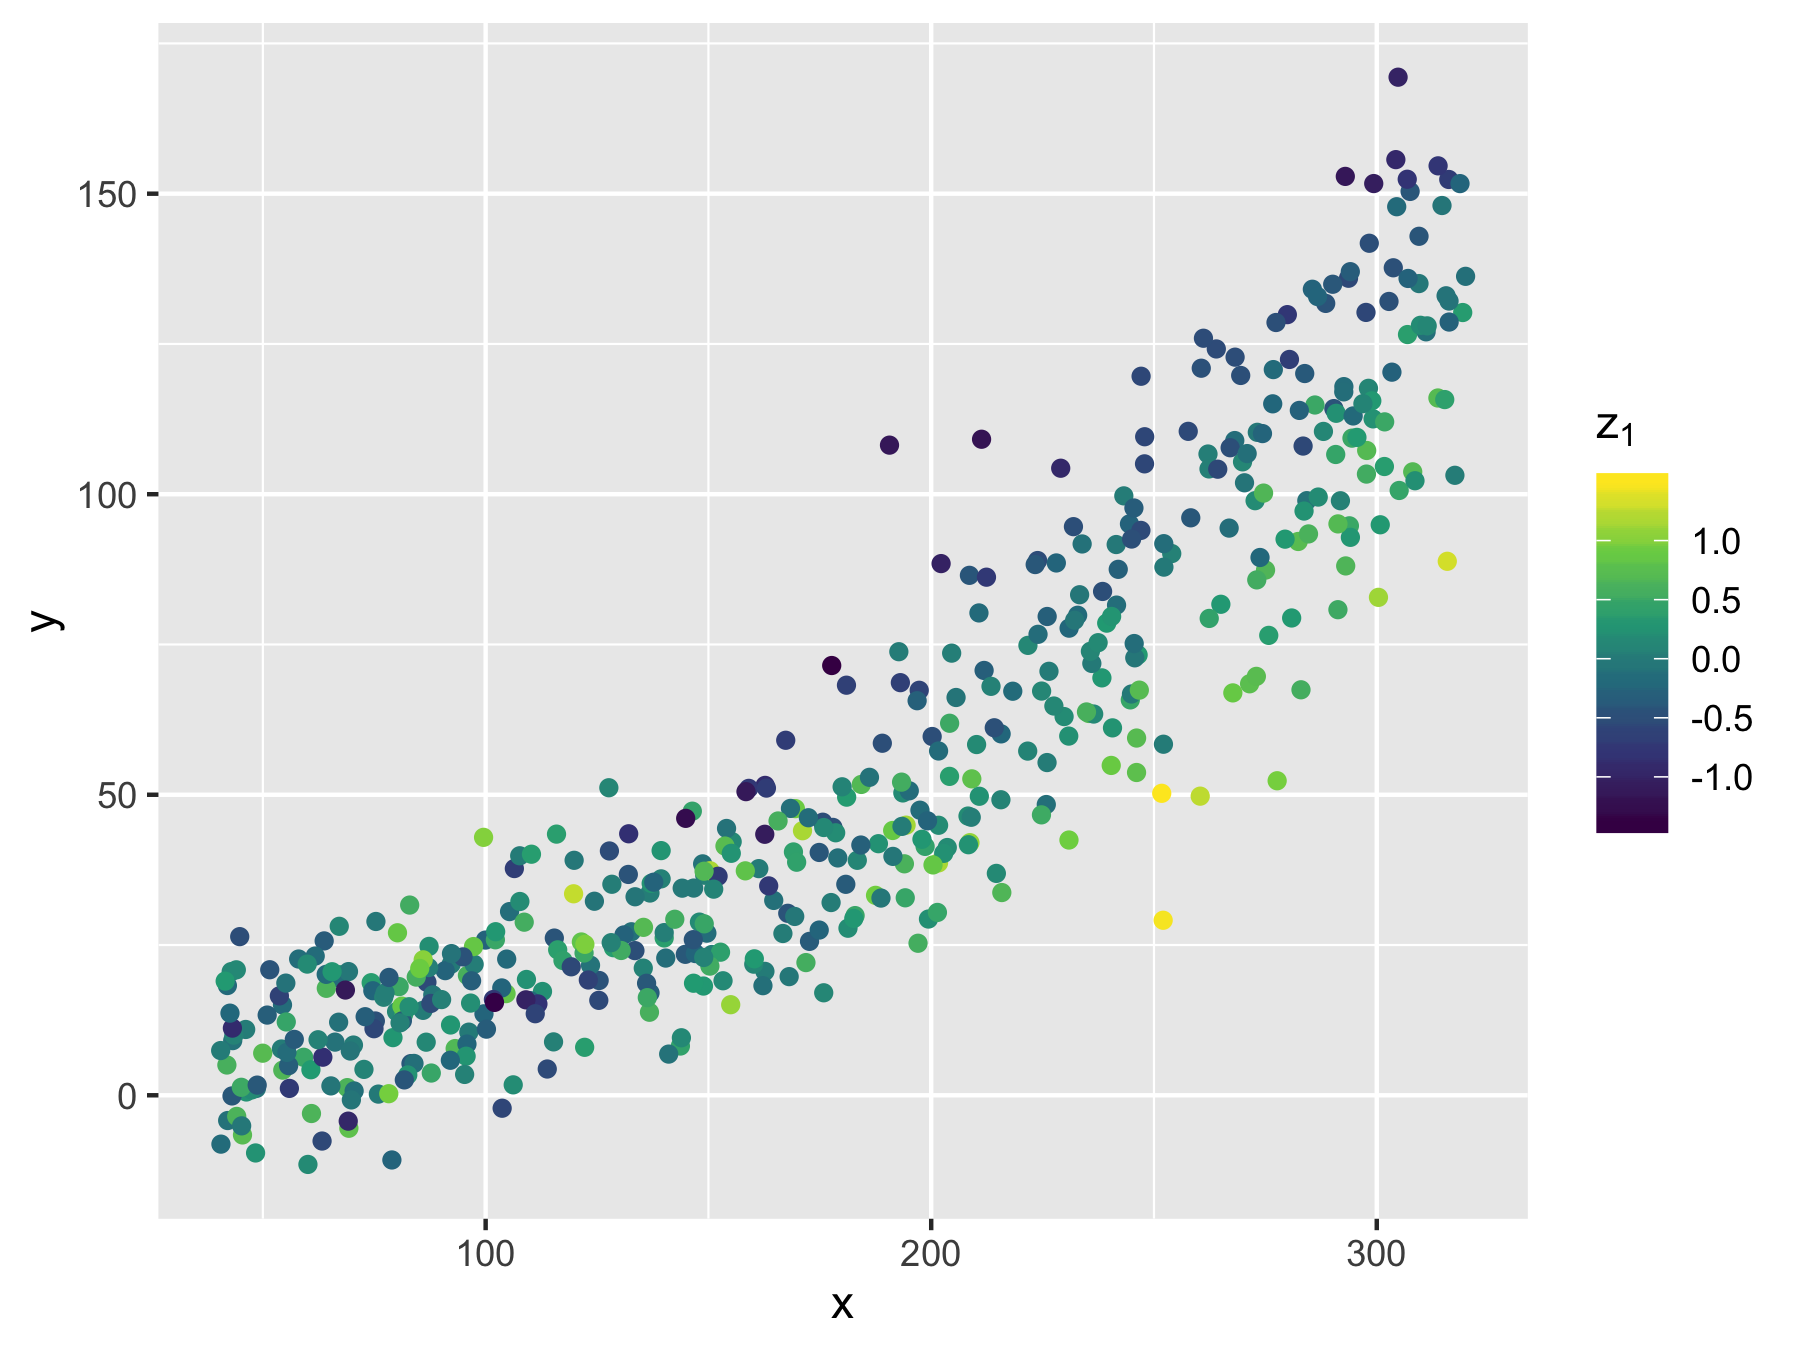
\includegraphics[width = 6 in]{PlotA_3.png}
    \caption{Example data generated under Setting 3 of simulation studies; $k = 0.5, N = 500, \delta_1 = 0.5, \sigma = 10$}
\end{figure}

\begin{figure}
    \centering
    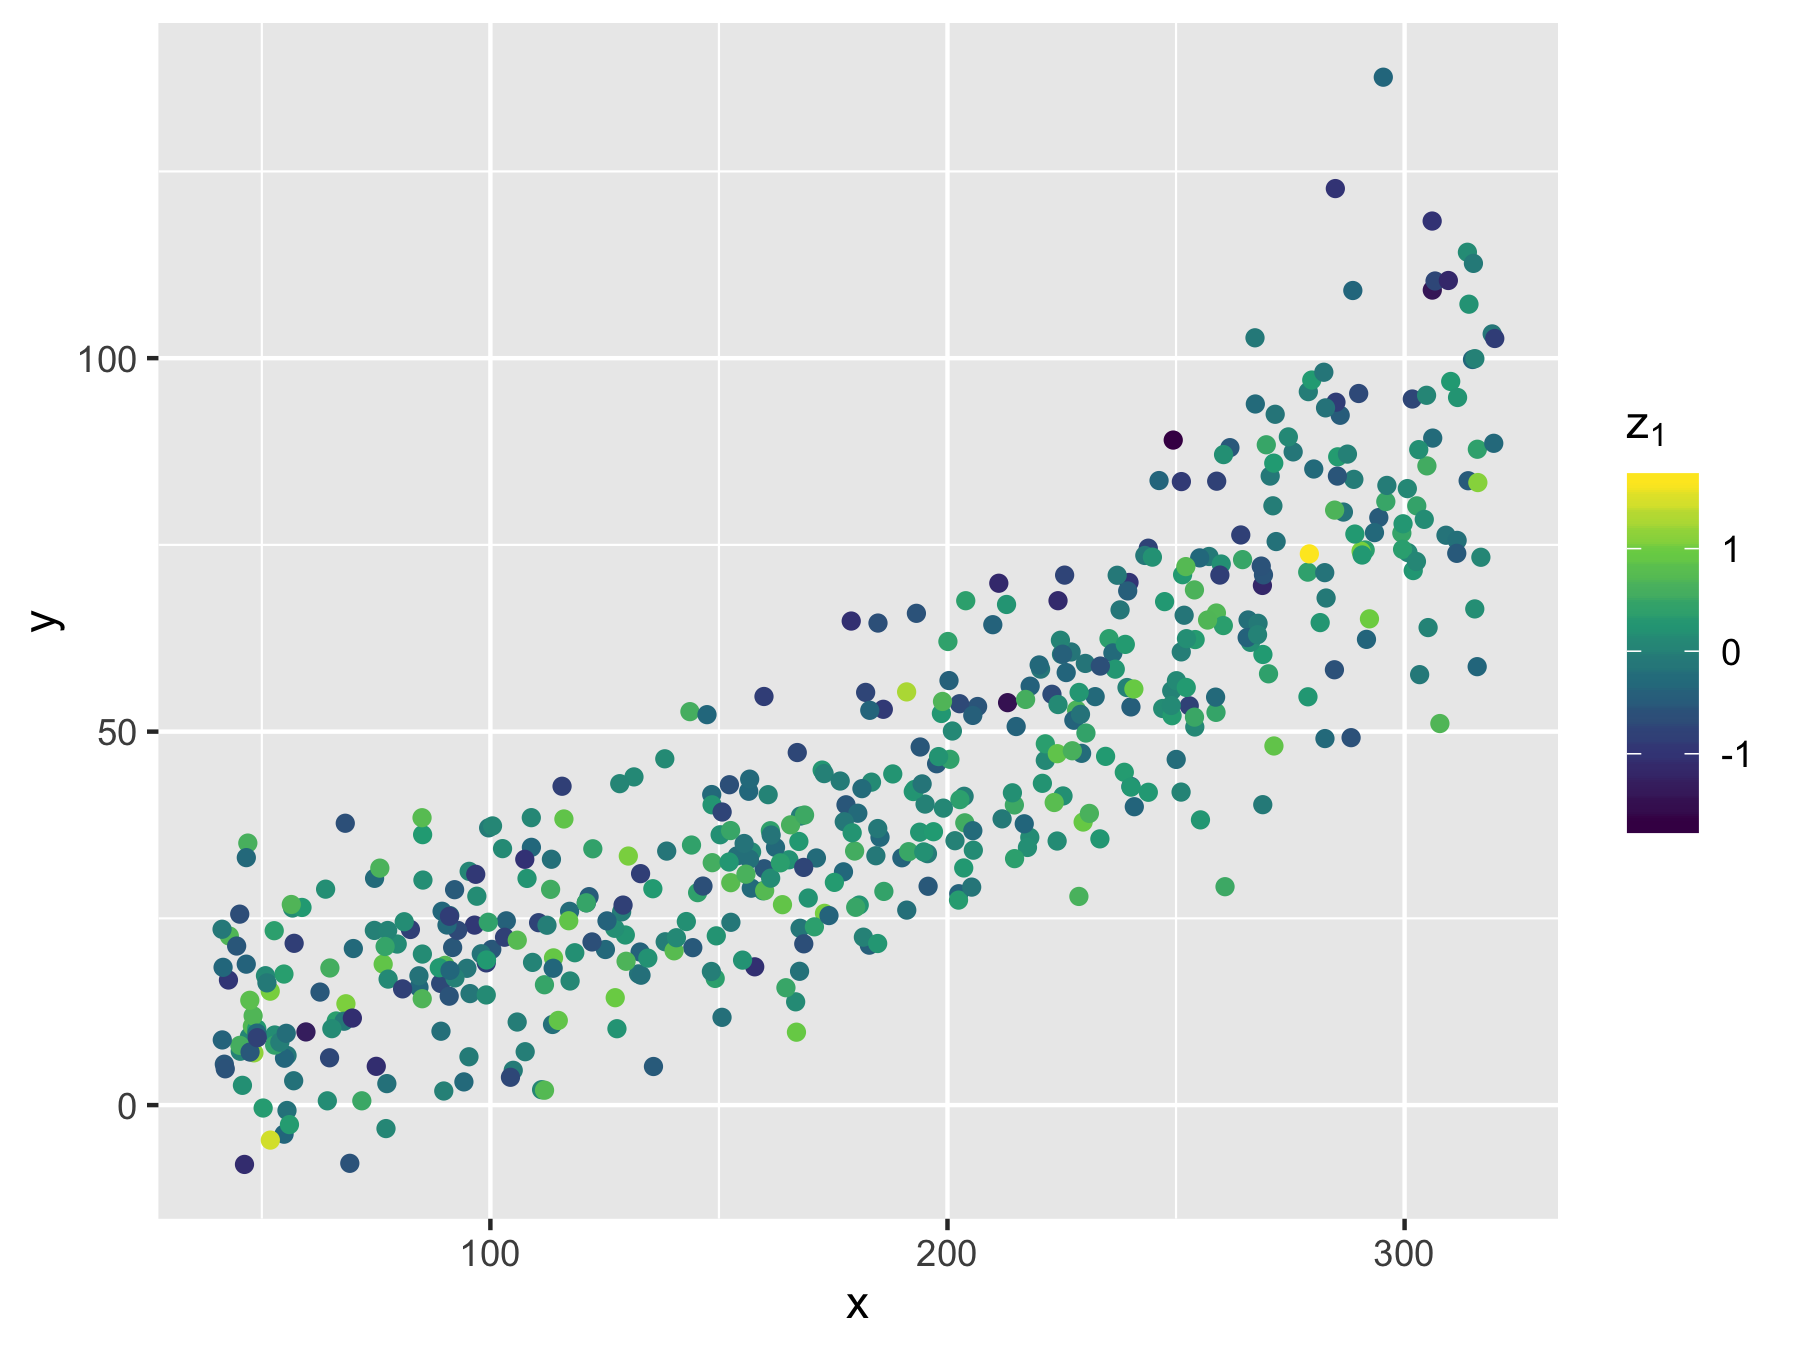
\includegraphics[width = 6 in]{PlotA_4.png}
    \caption{Example data generated under Setting 4 of simulation studies; $k = 0.5, N = 500, w = 0.4, \sigma = 10$}
\end{figure}

\begin{figure}
    \centering
    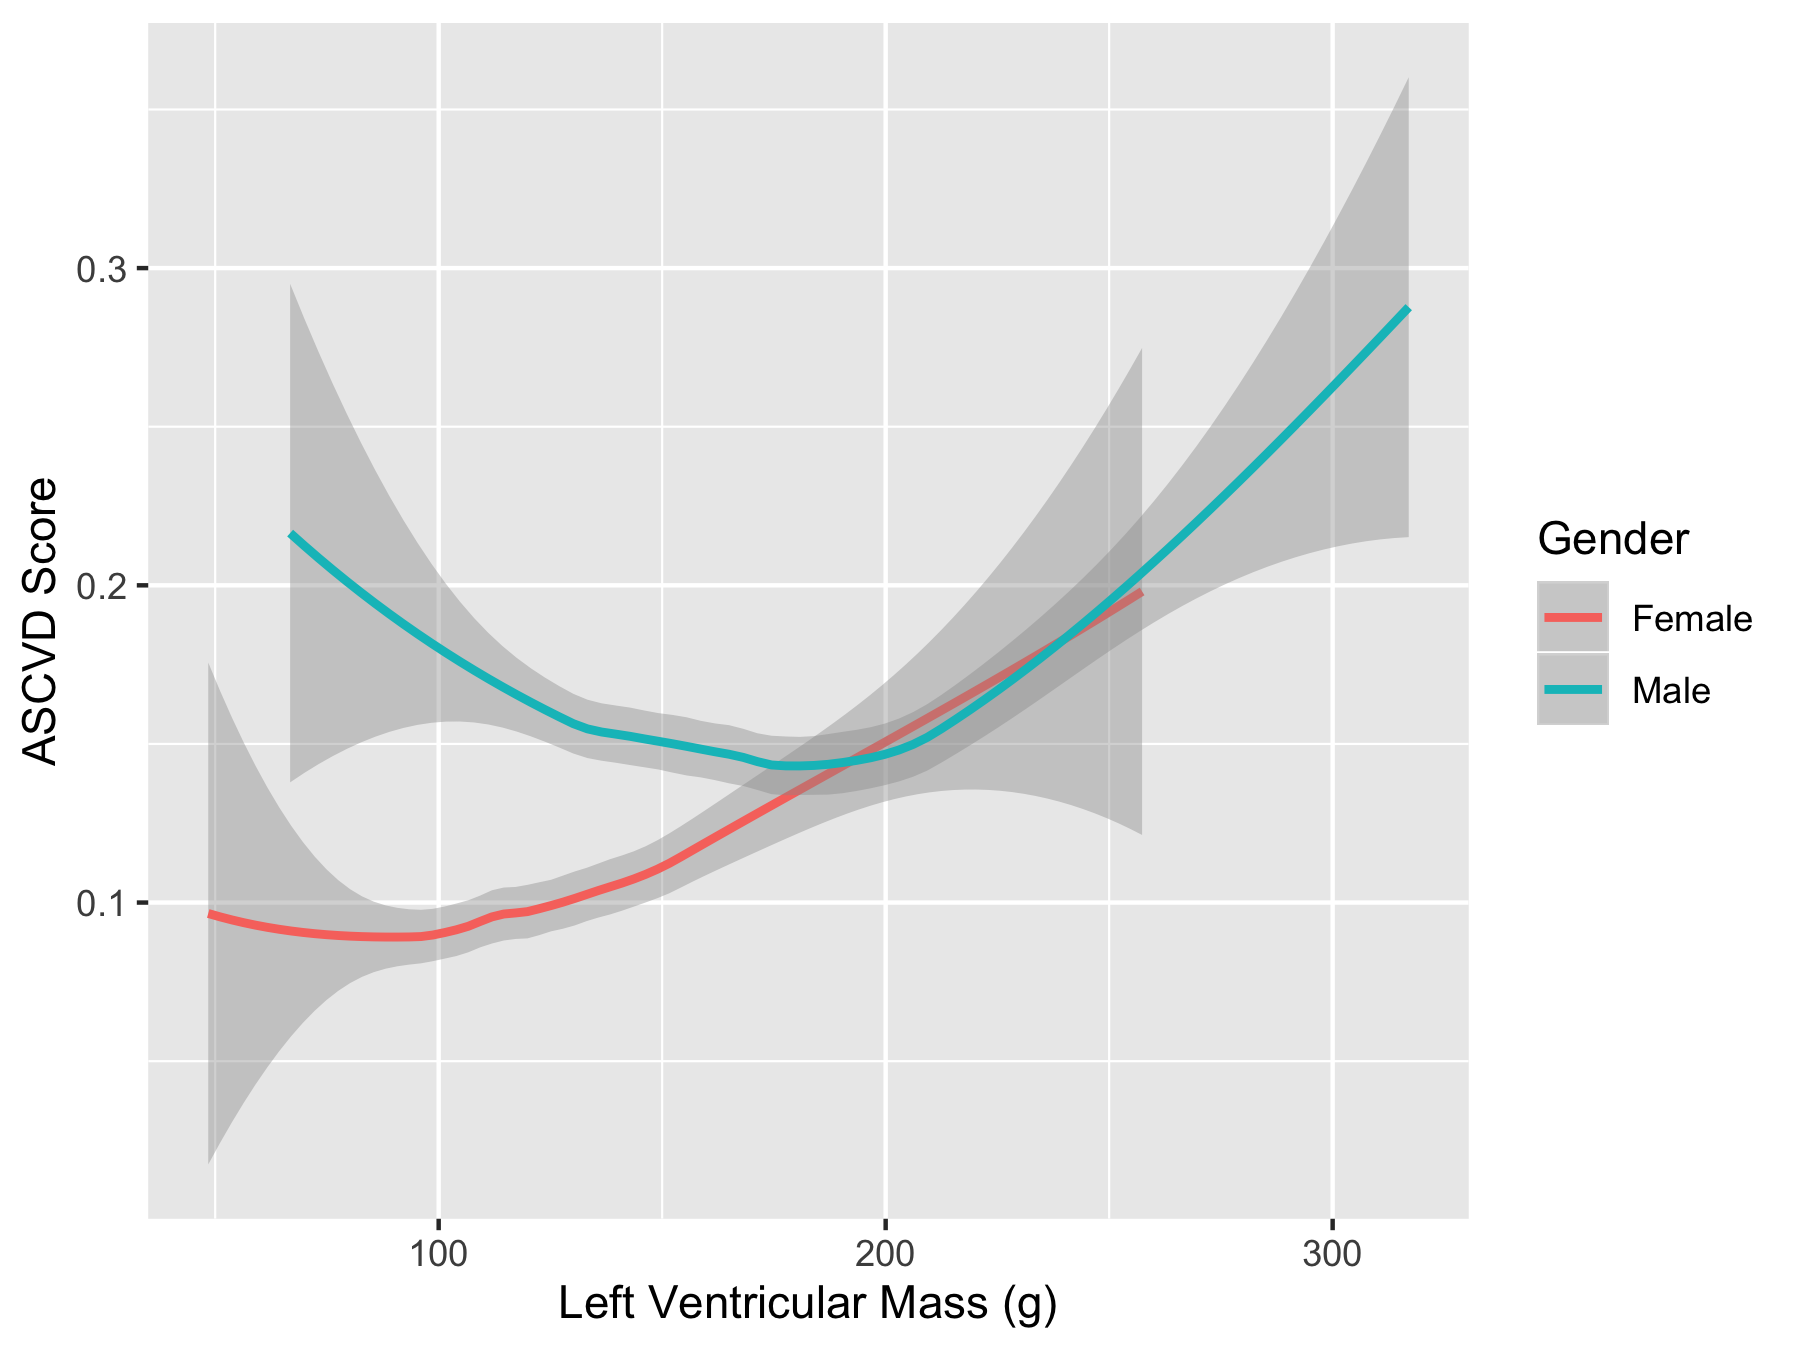
\includegraphics[width = 6 in]{PlotA_5.png}
    \caption{Smoother curves of ASCVD score vs. left ventricular mass by gender for selected MESA study subjects}
\end{figure}

\begin{figure}
    \centering
    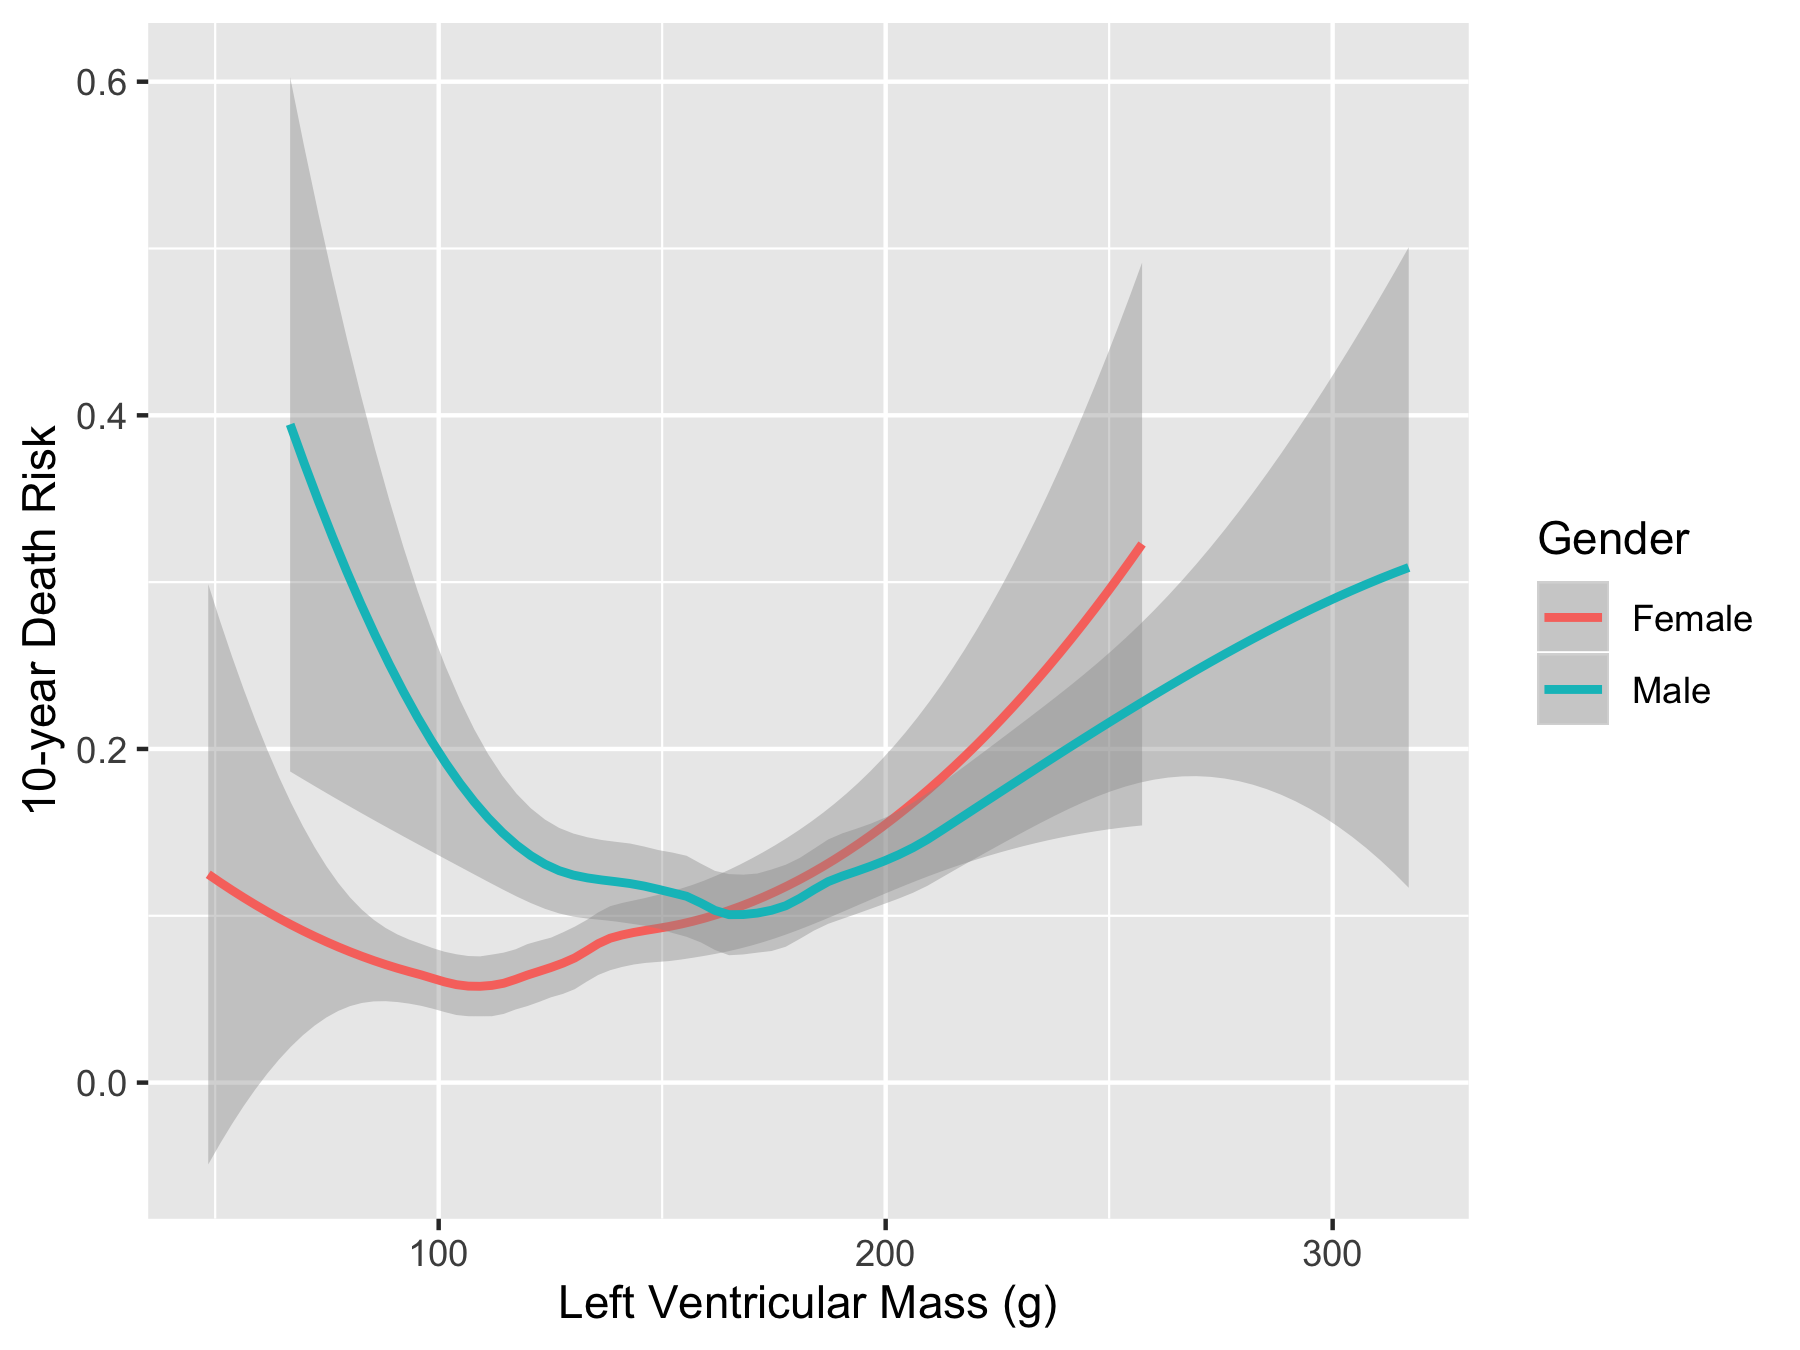
\includegraphics[width = 6 in]{PlotA_6.png}
    \caption{Smoother curves of 10-year death risk vs. left ventricular mass by gender for selected MESA study subjects}
\end{figure}

\begin{figure}
    \centering
    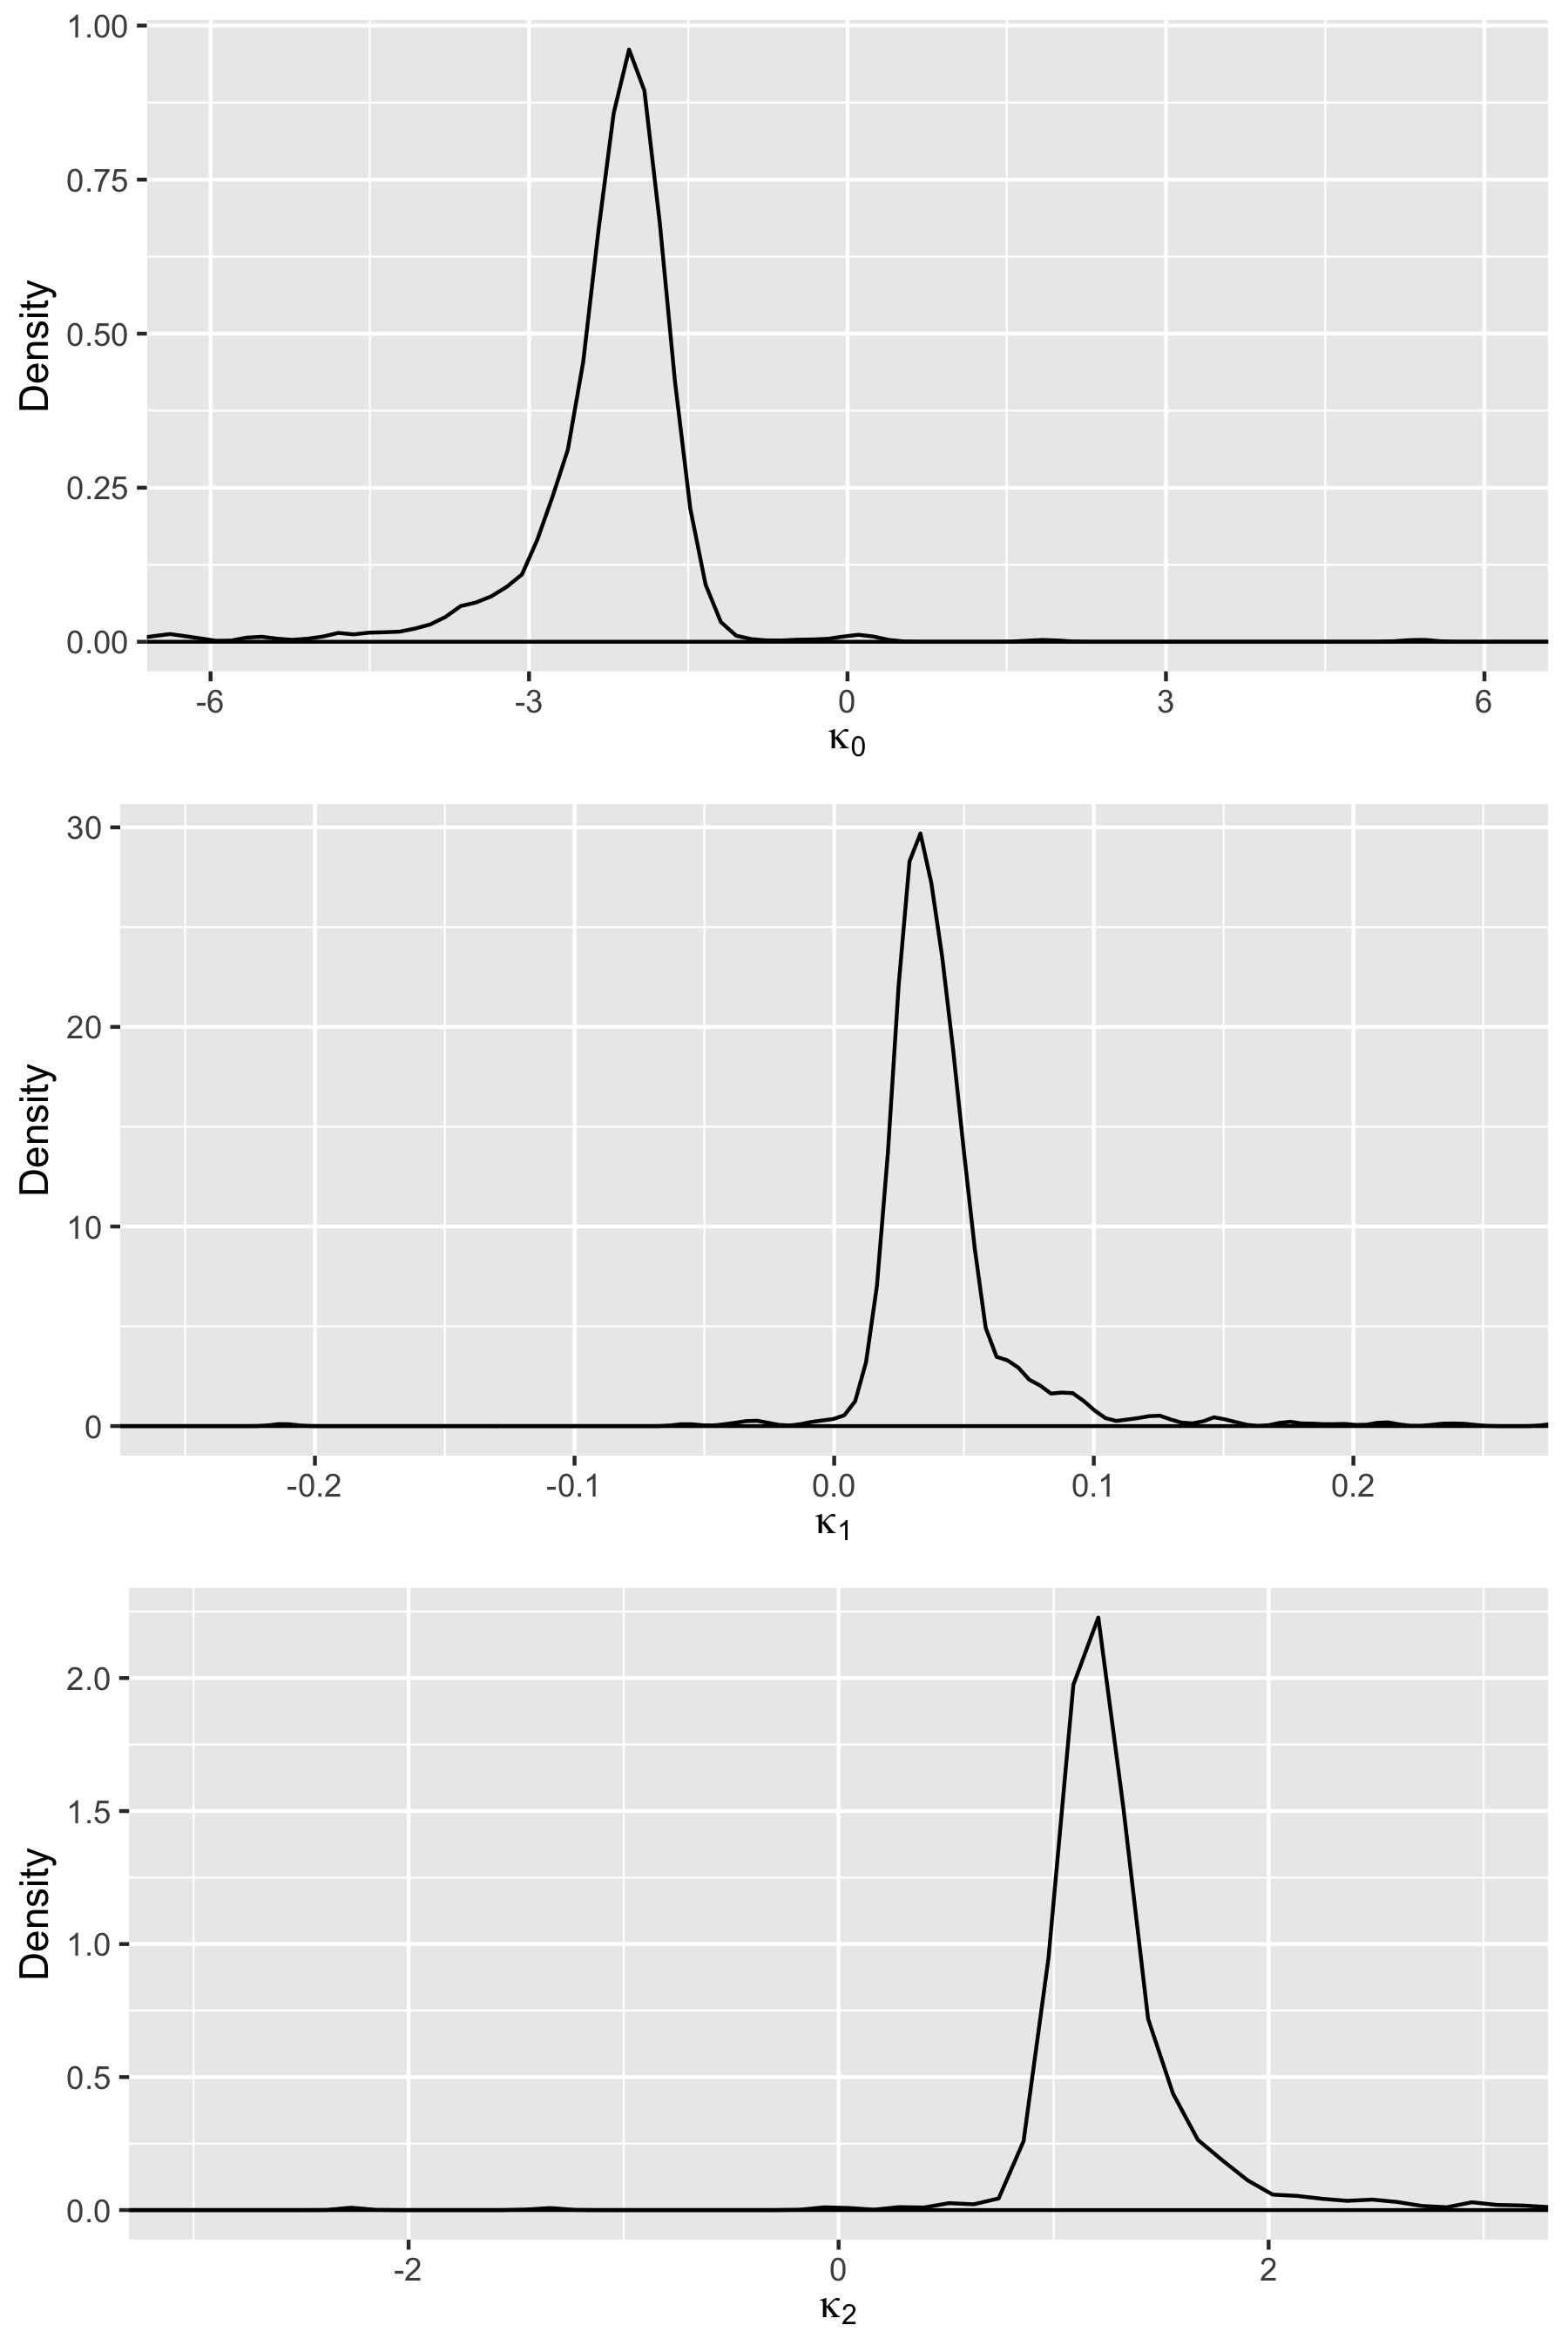
\includegraphics[width = 5.5 in]{PlotA_7.png}
    \caption{Kernel density estimators of bootstrap distribution of $\kappa$ parameters, with ASCVD score as outcome}
\end{figure}

\begin{figure}
    \centering
    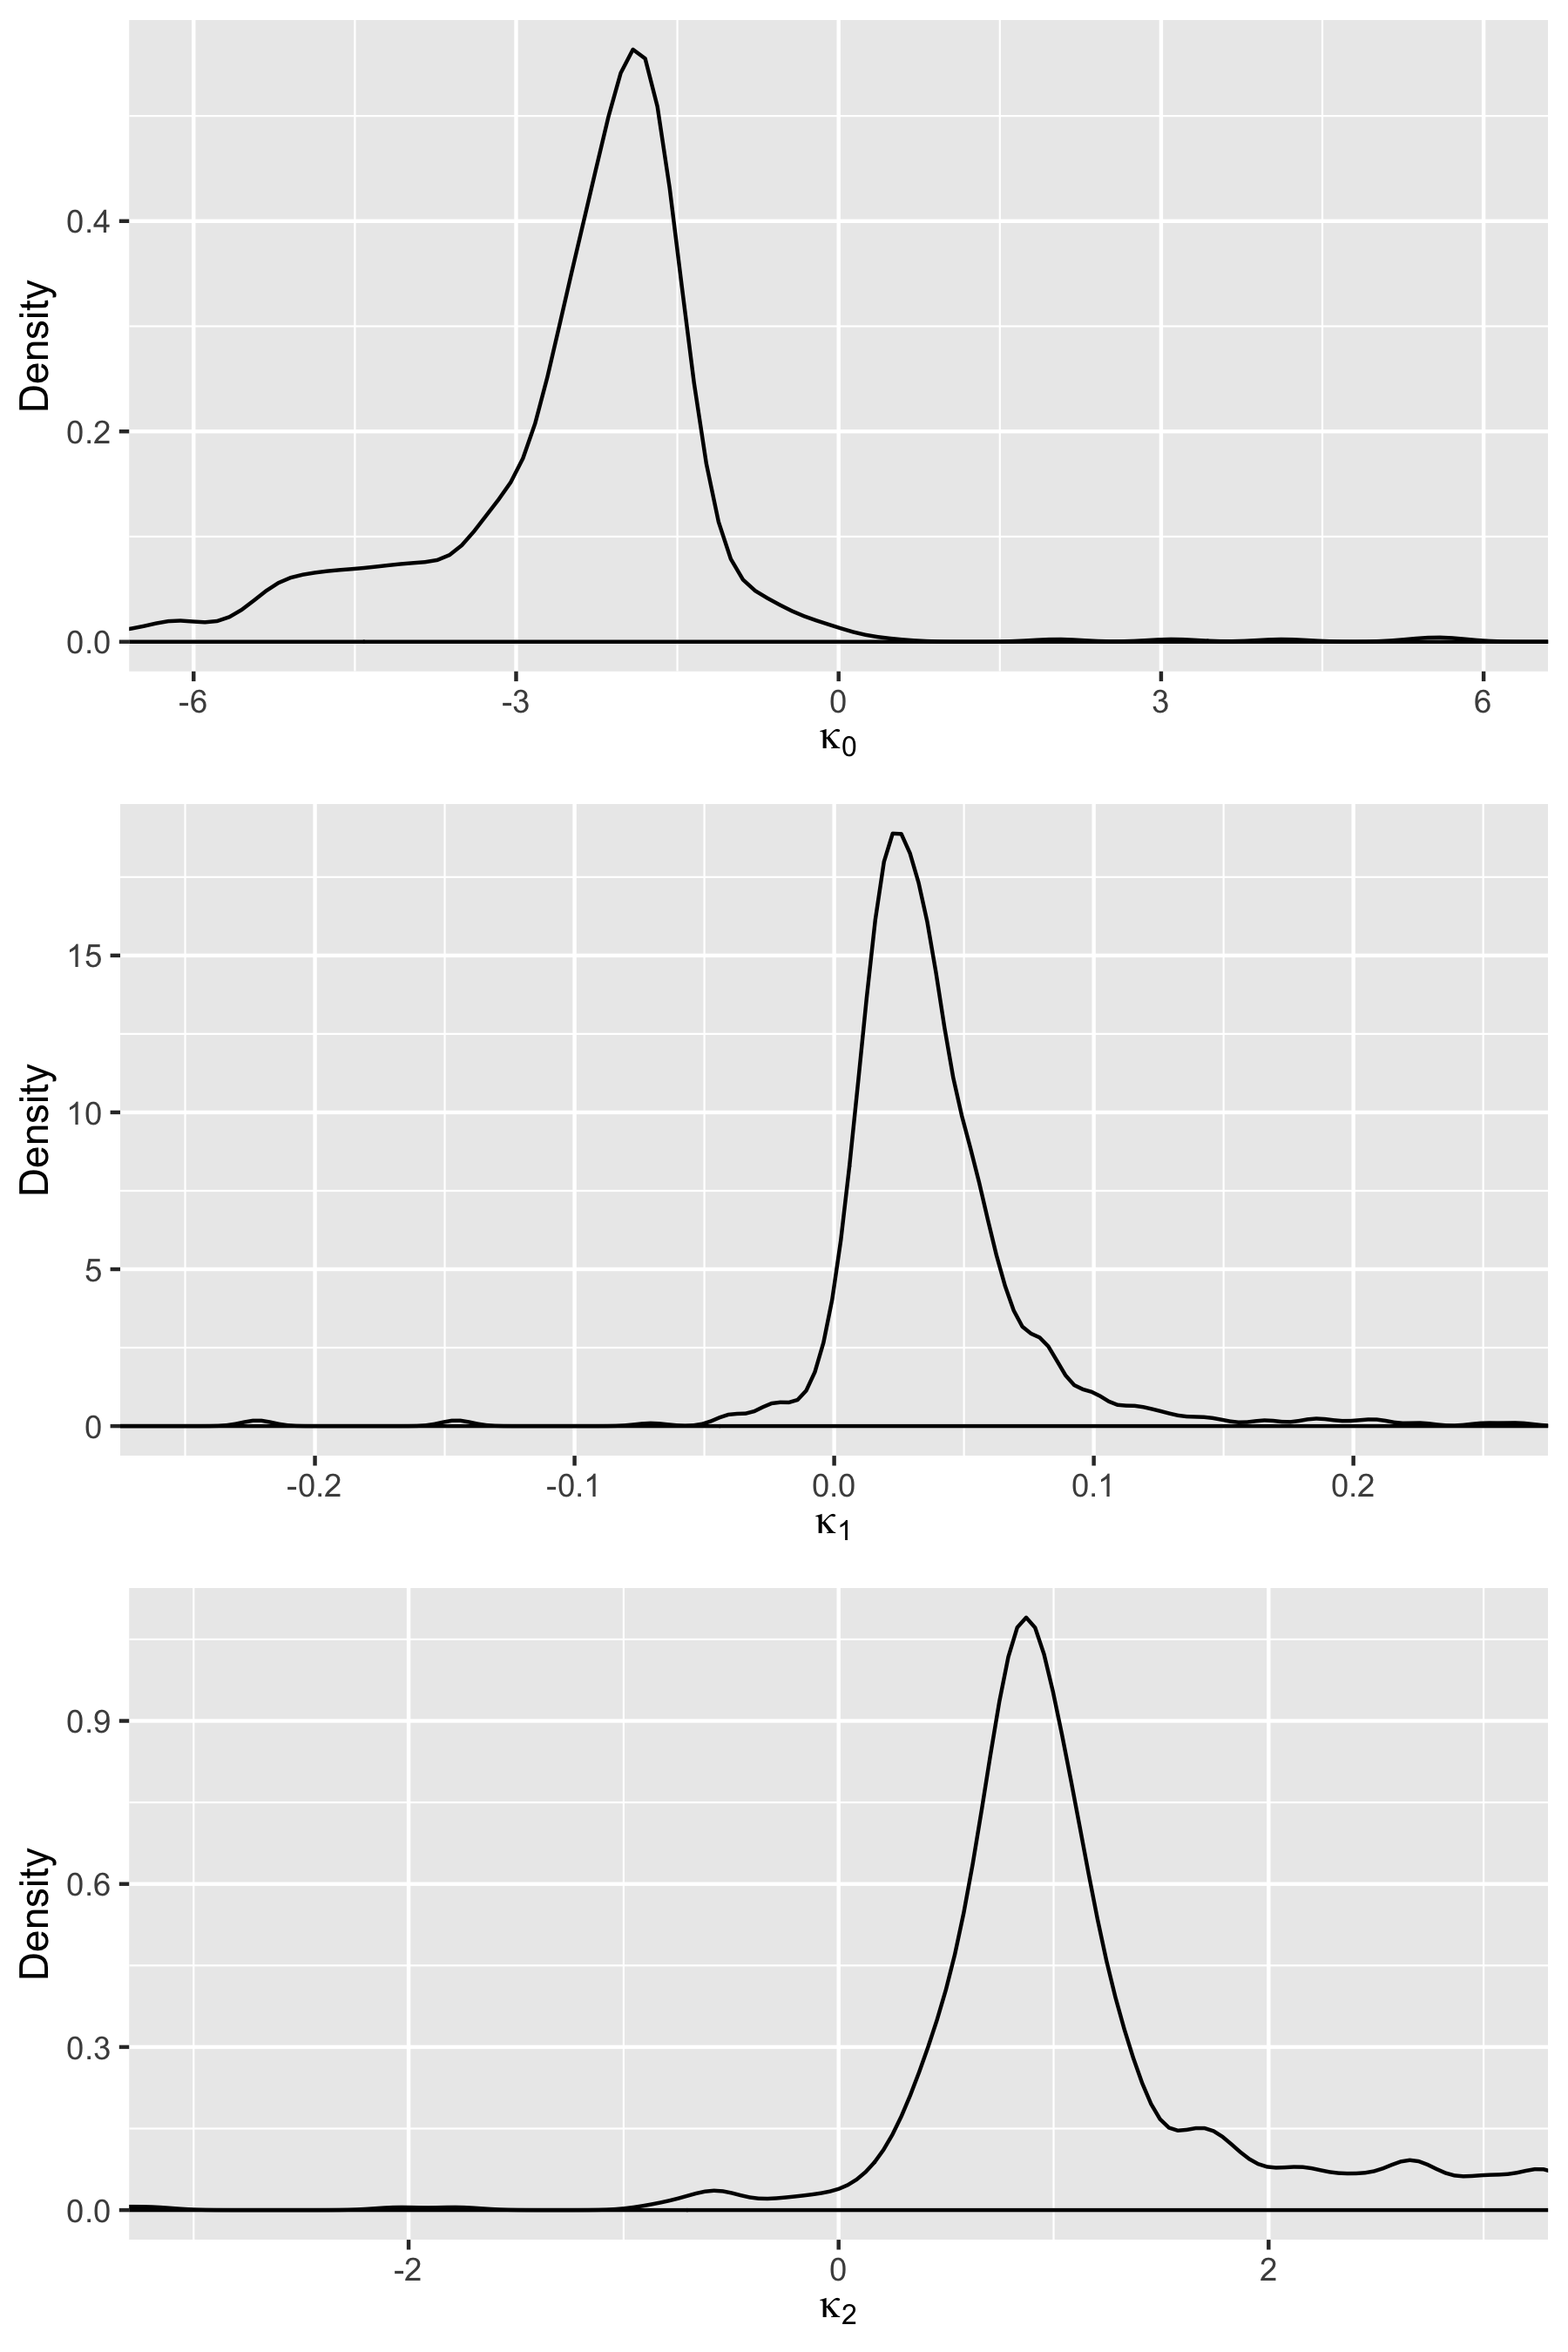
\includegraphics[width = 5.5 in]{PlotA_8.png}
    \caption{Kernel density estimators of bootstrap distribution of $\kappa$ parmeters, with 10-year truncated death as outcome}
\end{figure}

\end{document}
